% thesis.tex
%
% This file is root file for an example thesis written using the
% University of Wisconsin-Madison LaTeX Style file.
%
% It is provided without warranty on an AS IS basis.


%=====================================================================
% Document Style
%=====================================================================
% Choose only one of the following document classes:
%
% for a 12 Point UW PhD Thesis without Margin Check
\documentclass[12pt]{withesis}
%
% for a 10 Point UW PhD Thesis with Margin Check
%\documentclass[10pt,margincheck]{withesis}
%
% The margincheck option flags lines which overflow their hbox with a black
%  box at the end of the line.  This usually (but not always) indicates a
%  margin violation on the right margin.  Left margin violations aren't
%  indicated and if the margin violation is large enough, there isn't room
%  for the black box to be visiable.  
%
% This option can be also used in conjunction with the msthesis option.
%
% or for a 12 Point UW Masters Thesis
%\documentclass[12pt,msthesis]{withesis}
%
% or for a 10 Point UW Masters Thesis
%\documentclass[10pt,msthesis]{withesis}
%
% The msthesis option changes the page margins from 1" all around
% (the PhD format) to 1.25" left and 1" remaining margins (MS format).
% The defaults for degree and thesis are changed to be MS and thesis.
% These defaults can be overridden if the margins for the MS thesis
% are desired for other documents.

% To include optional packages, use the \usepackage command.
%  The package epsfig is used to bring in the Encapsulated PostScript
%    figures into the document.
%  The package times is used to change the fonts to Times Roman; however
%    because the times typewriter font looks odd, the original LaTeX
%    Computer Modern font is kept for the typewriter font using
%      \renewcommand{\ttdefault}{cmtt}
%    Note that Times Roman is a PostScript font and therefore, the document
%    cannot be correctly viewed from the *.dvi file.  It should be converted
%    to a *.ps file first and then viewed with a PostScript previewer...

\usepackage{geometry}
\geometry{margin=1.2in}

\usepackage{hyperref}

\usepackage{url}        % Not compatible with hyperref?
\usepackage{float}
\usepackage{graphicx}
\usepackage{amsmath}
\usepackage{color}
\usepackage{times}
\usepackage{verbatim}
\usepackage{xspace}
\usepackage{xfrac}

%\usepackage{listings}
%\usepackage{microtype} %does typographical voodoo to get rid of most overfull
                       %boxes. Ideally requires pdfTeX 1.4+, going directly
                       %to pdf. Don't use a DVI workflow.
\usepackage{balance}   %\balance keywork has to be included in the last page that
                       % will not be balanced, in the first column.
\usepackage{datetime}
\usepackage{morefloats}

\usepackage{caption}
\usepackage{subcaption}
\usepackage{multirow}

\usepackage{amssymb}% http://ctan.org/pkg/amssymb
\usepackage{pifont}% http://ctan.org/pkg/pifont


\usepackage{booktabs} % For formal tables
\usepackage{footnote}


\usepackage{enumitem}
\setlist[itemize]{leftmargin=*}
\usepackage{algpseudocode,algorithm,algorithmicx}

\newcommand{\nop}[1]{}

\algnewcommand\algorithmicinput{\textbf{Input:}}
\algnewcommand\Input{\item[\algorithmicinput]}
\algnewcommand\algorithmicoutput{\textbf{Output:}}
\algnewcommand\Output{\item[\algorithmicoutput]}

\let\oldReturn\Return
\renewcommand{\Return}{\State\oldReturn}

%=======================================================================
% Remove the following lines if appendix tables or figures are present.
% The suppress writing the auxiliary information which appears in the
% list of tables or list of figures.
%
\noappendixtables                % Don't have appendix tables
\noappendixfigures               % Don't have appendix figures


\begin{document}

%\newgeometry{left=1in,right=1in,bottom=1in,top=1in}
% Choose your bibliography style
% plain is the basic style, others include ieeetr, siam, asm, etc
%\bibliographystyle{plain}


% prelude.tex
%   - titlepage
%   - dedication
%   - acknowledgments
%   - table of contents, list of tables and list of figures
%   - nomenclature
%   - abstract
%============================================================================


\clearpage\pagenumbering{roman}  % This makes the page numbers Roman (i, ii, etc)



% TITLE PAGE
%   - define \title{} \author{} \date{}
\title{Improving Datacenter Network Performance via the Intelligent Network Edge}
\author{Lei Kang}
\date{}
%   - The default degree is ``Doctor of Philosophy''
%     (unless the document style msthesis is specified
%      and then the default degree is ``Master of Science'')
%     Degree can be changed using the command \degree{}
\degree{Doctor of Philosophy}
%   - The default is dissertation, unless the document style
%     msthesis was specified in which case it becomes thesis.
%     If msthesis is specified for the MS margins, you can
%     still have a dissertation if you specify \disseration
%\disseration
%   - for a masters project report, specify \project
%\project
%   - for a preliminary report, specify \prelim
%\prelim
%   - for a masters thesis, specify \thesis
\thesis
%   - The default department is ``Electrical Engineering''
%     The department can be changed using the command \department{}
\department{Computer Sciences}
%   - once the above are defined, use \maketitle to generate the titlepage
\oralexamdate{5/1/2018}
\committeeone{Suman Banerjee, Professor, Computer Science}
\committeetwo{Srinivasa A. Akella, Professor, Computer Science}
\committeethree{Eric J. Rozner, Research Staff Member, IBM Research}
\committeefour{Michael M. Swift, Associate Professor, Computer Science}
\committeefive{Xinyu Zhang, Assistant Professor, Electrical and Computer Engineering}
\date{2018}


\maketitle

% COPYRIGHT PAGE
%   - To include a copyright page use \copyrightpage
\copyrightpage

% DEDICATION
\begin{dedication}
\emph{To my loved ones}
\end{dedication}

% ACKNOWLEDGMENTS
\begin{acknowledgments}

It has been a long but rewarding journal at UW-Madison.

First of all, I would like to thank my Ph.D. advisor, Prof. Suman Banerjee. 
He has done an amazing job in guiding my graduate studies, transforming me
from a college graduate without knowing what to do, to a confident Ph.D. with
solid skills at hands. 
He changed me from a paper driven researcher to a problem solving researcher. 
I deeply appreciate the time, patience, care, 
and support Prof. Banerjee has devoted to guiding my professional
development, along with the help on many personal matters. 
 
I would like to thank the members of my thesis committee, TBD. 
Their valuable suggestions and comments greatly improved this thesis.
 
I would like to thank my MPhil advisor, Prof. Lionel Ni. 
He is a decent and kind man. 
He always take care of his students, in every way that is possible, 
while he is very busy with academic and administrative affairs. 


I would like to thank my internship mentors, Bozidar

 
I would like to thank my research collaborators, 
Peng Liu,
Bozhao Qi,
Wei Zhao,
Dan Janecek,
. 
Working with these brilliant people is a great gift to me. 
I am also quite fortunate to have great friends that I can hang out with and have
beer together: 
Keqiang He,
Suli Yang,


Last but definitely the most important one, my wife.  


\end{acknowledgments}

% CONTENTS, TABLES, FIGURES
\tableofcontents
%%\listoftables
%%\listoffigures



\advisorname{Suman Banerjee}
\advisortitle{Professor}



\begin{abstract}



Vehicles bring us travel convenience as well as many problems 
such as environment pollution, road congestion and fatalities. 
We propose building smart in-vehicle systems and smartphone enabled
vehicular applications to provide various types of 
assistance to remedy these issues. 
Such systems sense and model vehicle dynamics from vehicle parameters and
third party sensors, based on which they provide guidance
and control to assist human drivers and achieve better driving performance. 
EcoDrive is one such system we built that conduct fuel consumption sensing and control 
to improve fuel efficiency and reduce carbon emissions. 
EcoDrive models instant fuel consumption based on vehicle 
parameters collected from On-board diagnostics (OBD) port. 
According to the model, it controls the gas pedal position sensor
to adjust fuel injection rate according to road segment distance 
and speed limit. 
By using careful control of fuel injection rate, it is able
to improve fuel efficiency comparing to human drivers. 
We also implemented a smartphone vehicular application, called DriveSense, 
that senses vehicle dynamics by built-in sensors and provide feedback to drivers 
on aggressive events to improve their driving safety awareness.
Sensing vehicle dynamics by smartphone sensors require coordinate alignment
between the smartphone and the car. 
We found that even gentle road slopes may cause 
severe coordinate misalignment and acceleration over/under estimation. 
To resolve these problems, we propose slope-aware
coordinate alignment algorithm and linear acceleration
estimation method to reduce alignment training time and improve
linear acceleration estimation accuracy.  
Based on our past experiences on in-vehicle systems and driving behavior study, 
we propose two future work to further improve driving safety 
and efficiency by utilizing smartphone sensors. 
First, we propose to evaluate the performance of smartphone GPS and 
IMU sensors for capturing driving behaviors, 
and examine the benefits when combining GPS and IMU sensors.
Second, we propose to combine smartphone cameras, GPS and IMU sensors to detect driver phone use. 

\end{abstract}


\clearpage\pagenumbering{arabic} % This makes the page numbers Arabic (1, 2, etc)
                % Title page, abstract, table of contents, etc
%*******************************************************************************
%*********************************** First Chapter *****************************
%*******************************************************************************

\chapter{Introduction} 


Vehicle makes our life easier by bringing us travel convenience, 
but it also produces problems such as travel cost, carbon pollution, 
car accident and road congestion.
In 2015, about 140.43 billion gallons of gasoline were consumed in the United States. 
Also, according to the US Census Bureau, there are about ten million car accidents every year.
It has been shown that most car accidents are mainly 
caused by dangerous driving behaviors and human mistakes \cite{progressive}. 
These problems are caused by the lack of understanding, monitoring 
and careful control on vehicle dynamics. 
Better understanding and control on vehicle dynamics
can not only reduce car accidents \cite{progressive}, 
but also improve fuel efficiency \cite{morganstanley2013}. 


There has been active efforts to achieve better understanding on
human driving behaviors and better control on vehicles. 
One such example is to use driverless car system to 
replace human drivers \cite{googledriverlesscar, kumar2012carspeak,
urmson2008autonomous,litman2013autonomous}. 
However, it takes time for self-driving systems to be robust enough to 
replace traditional vehicles. 
Also, it is unlikely that self-driving
systems are going to ever achieve perfect accuracy under all
conditions.
Meanwhile, some researchers are using existing technologies to assists human drivers
in user-operated vehicles are more critical for safe 
and efficient driving activities \cite{you2013carsafe, wang2013sensing, chen2015invisible, uber}. 
Also, there are in-vehicle systems that assist human drivers with some driving functionalities, 
e.g., cruise control \cite{bengtsson2001adaptive, cruise_control} and emergence braking system \cite{emergency_brake} etc. 
However, there are many questions that have not been answered: 
what is the accuracy of smartphone sensors to capture driving behaviors?
how to assist human drivers to achieve fuel efficient and safe driving?
how to make self-driving systems more reliable? 


With many open questions in mind, we ask a high-level question in this proposal: 

\emph{how can we build sensing and control system blocks for modern vehicles to
monitor, assist or even replace human drivers in
improving driving performance and experience?}


To answer this question, we explore the sensing and control capabilities
of commodity hardwares and how to utilize them on modern vehicles. 
For example, we can use smartphone to sense and capture 
various driving behaviors, 
based on which we can evaluate driving performance. 
We can also access vehicle parameters from OBD 
port \cite{obd} to evaluate our driving behavior detection algorithms. 
We implemented a smartphone application called DriveSense to collect
data and verify our algorithms. 
We also present a control system called EcoDrive that 
leverages drive-by-wire technology to control fuel injection
rate to find a tradeoff between travel time and fuel efficiency. 
To handle occational self-driving system failures, 
we present a live streaming and remote control framework
called RTDrive to augment self-driving systems. 


\section{DriveSense}



Smartphone-based sensing has opened up a whole gamut of applications and services
for road safety, such as driving behavior and driver distraction monitoring. 
One such application is the ability to independently monitor driving behavior --- how well is one
driving the vehicle, e.g., aggressive driving actions, such as rough acceleration, hard brakes, and lane changes, and more.
The popularity of smartphones and built-in Inertial Measurement Unit (IMU) sensors enable
a low-cost way of monitoring such behaviors and actions.
For example, Cambridge Mobile Telematics \cite{cmt} 
develops a smartphone
app to capture driving behaviors and monitor driver
distractions.
The well-known ride-sharing company Uber announced
it will start tracking Uber drivers' driving behaviors
with their smartphones and give them feedbacks that are more detailed than 
the five-star rating customers leave for each driver \cite{uber}.

The general approach to monitoring such vehicle motion (and drive) parameters is to use an accelerometer in a mobile device
 to measure the three-dimensional acceleration
and using a gyroscope to measure the three-dimensional relative rotation speed.
The accelerometer can be used to sense vehicular speed \cite{hansenspeed}
by eliminating estimation errors at reference points where 
ground truth vehicular speed is known.
The gyroscope can be used to detect turns to determine
driver phone use by comparing centripetal accelerations with 
a reference point \cite{wang2013sensing}, 
and it can also be used to track drivers' 
other steering activities \cite{chen2015invisible}.
Calculating the exact orientation of the phone is an important step in enabling estimation of such motion parameters.
Prior work has dealt with different variants of this problem ---  the absolute coordinates estimation problem (orientation relative
to flat earth surface)  \cite{zhou2014use}
and the relative coordinates estimation problem (orientation relative to the orientation of the vehicle which depends on 
the grade and slope of the road) \cite{wang2013sensing, chen2015invisible}.
Both are challenging tasks due to the low accuracy 
and accumulated errors of IMU sensors \cite{zhou2014use}.
Most in-vehicle applications use the relative coordinates estimation 
and depend on coordinate alignment,
which essentially aligns the coordinates of the smartphone to the car \cite{wang2013sensing, chen2015invisible, hansenspeed}. 
In our evaluation, we found that such prior work is not able to accurately estimate
road slope gradients which leads to increased errors in estimating vehicle motion
parameters. Further, the coordinate alignment process usually needs time to
converge and a fast convergence time is desirable in many real-time settings.

\iffalse
But none of those work addressed the problems caused by road slope
and the method to estimate slope gradients before and after coordinate
alignments.
Also, it is still an open question that how fast 
alignment algorithm can converge, e.g., if an algorithm requires the whole
trip to train the algorithm, then it can not be used in real-time applications for short trips.
\fi


In this section, we study the impact of road slopes on estimating various vehicle motion
parameters, especially the acceleration related ones. This is the central problem for
vehicle motion sensing using such mobile devices because many roads are never perfectly
level and even gentle slope of roads can lead to significant inaccuracies.
Investigating this further, we find that there
are three related issues.
First, we use a real-world driving trace to show that
even a perfectly aligned smartphone may overestimate or
underestimate brakes and accelerations due to the gravitational
effect.
When a car is parked on a slope, the linear acceleration
of the heading direction should be zero, 
but the accelerometer will 
sense the gravity component  in the same direction and conclude
the car is accelerating or decelerating on upslope or downslope. 
Therefore, the heading direction component of the accelerometer may be overestimated or underestimated.
Second, we also show that the gravitational effect can prolong the training time
of coordinate alignment and lower alignment accuracy. 
So, it is necessary to estimate the slope gradients even before
coordinate alignment is fully conducted.
Third, estimating slope gradients by gyroscope is challenging due
to the low accuracy of the IMU sensors \cite{zhou2014use}.


To overcome these challenges, we designed a software module that 
can reduce coordinate alignment training time by utilizing selective
training and combining multiple training segments with different weights. 
We also improve coordinate alignment accuracy by 
improving slope gradient estimation at coordinate alignment time.
We believe reducing training time can enable real-time applications like 
aggressive driving behavior warning.
To estimate slope gradients after alignment, 
we use sensor fusion and opportunistic calibration.
Provided that no alignment is perfect, 
we eliminate errors of gyroscope and accelerometer caused by
misalignment.
We only use calibration segment,
which refers to the road segments that accelerometer can produce accurate gradient estimation,
to calibrate gyroscope. 
Compared to the state of the art, our coordinate alignment module can converge much 
faster and our linear acceleration estimation module can achieve better accuracy. 


\nop{
\textbf{Contributions}. We design a smartphone-based system to improve the accuracy of estimating
vehicle motion parameters. 
We illustrate that road gradients, even gentle ones,
can cause acceleration overestimation or underestimation 
due to the gravitational effect.
They also have a great impact on coordinate alignment. 
We implement a software module that can reduce coordinate alignment
training time to enable real-time estimation of these parameters.
It can also estimate slope gradient before and after coordinate alignment
by combining the estimation results from accelerometer and gyroscope. 
By removing the gravity components, it is able to capture vehicle motion parameters
with greater accuracy than the state of the art,  
comparing with ground truth speed readings from the 
in-vehicle on-board diagnostics (OBD) port \cite{obd}.
The coordinate alignment is faster than the existing state of the art alternatives.
We evaluate our solution by using traces across highways and urban city roads of about 10,000 miles.
}








\section{EcoDrive}



The fuel conumption and carbon pollution caused by 
driving activities are drawing more and more attentions. 
In 2013, the White House issued a climate action plan to reduce fuel consumption
and carbon pollution \cite{whitehouse2013}. 
In the same year, Morgan Stanley reported that 
there will be \$158 billion annual savings in the US 
if all cars adopted smooth driving styles \cite{morganstanley2013}. 
We introduce a driver assistance system, called EcoDrive, 
that can improve the fuel efficiency of a vehicle's drive by sensing, computing, 
and actuating the acceleration behavior of the vehicle in an autonomous manner, 
by modeling properties of the vehicle, road conditions, and driving actions. 
With the global push for improving fuel efficiency of vehicles to 
reduce consumptions and carbon emissions, 
we believe solution such as ours can be one of many important mechanisms to meet such a goal.


\begin{figure}[t]
\begin{center}
\vspace{-0.5cm}
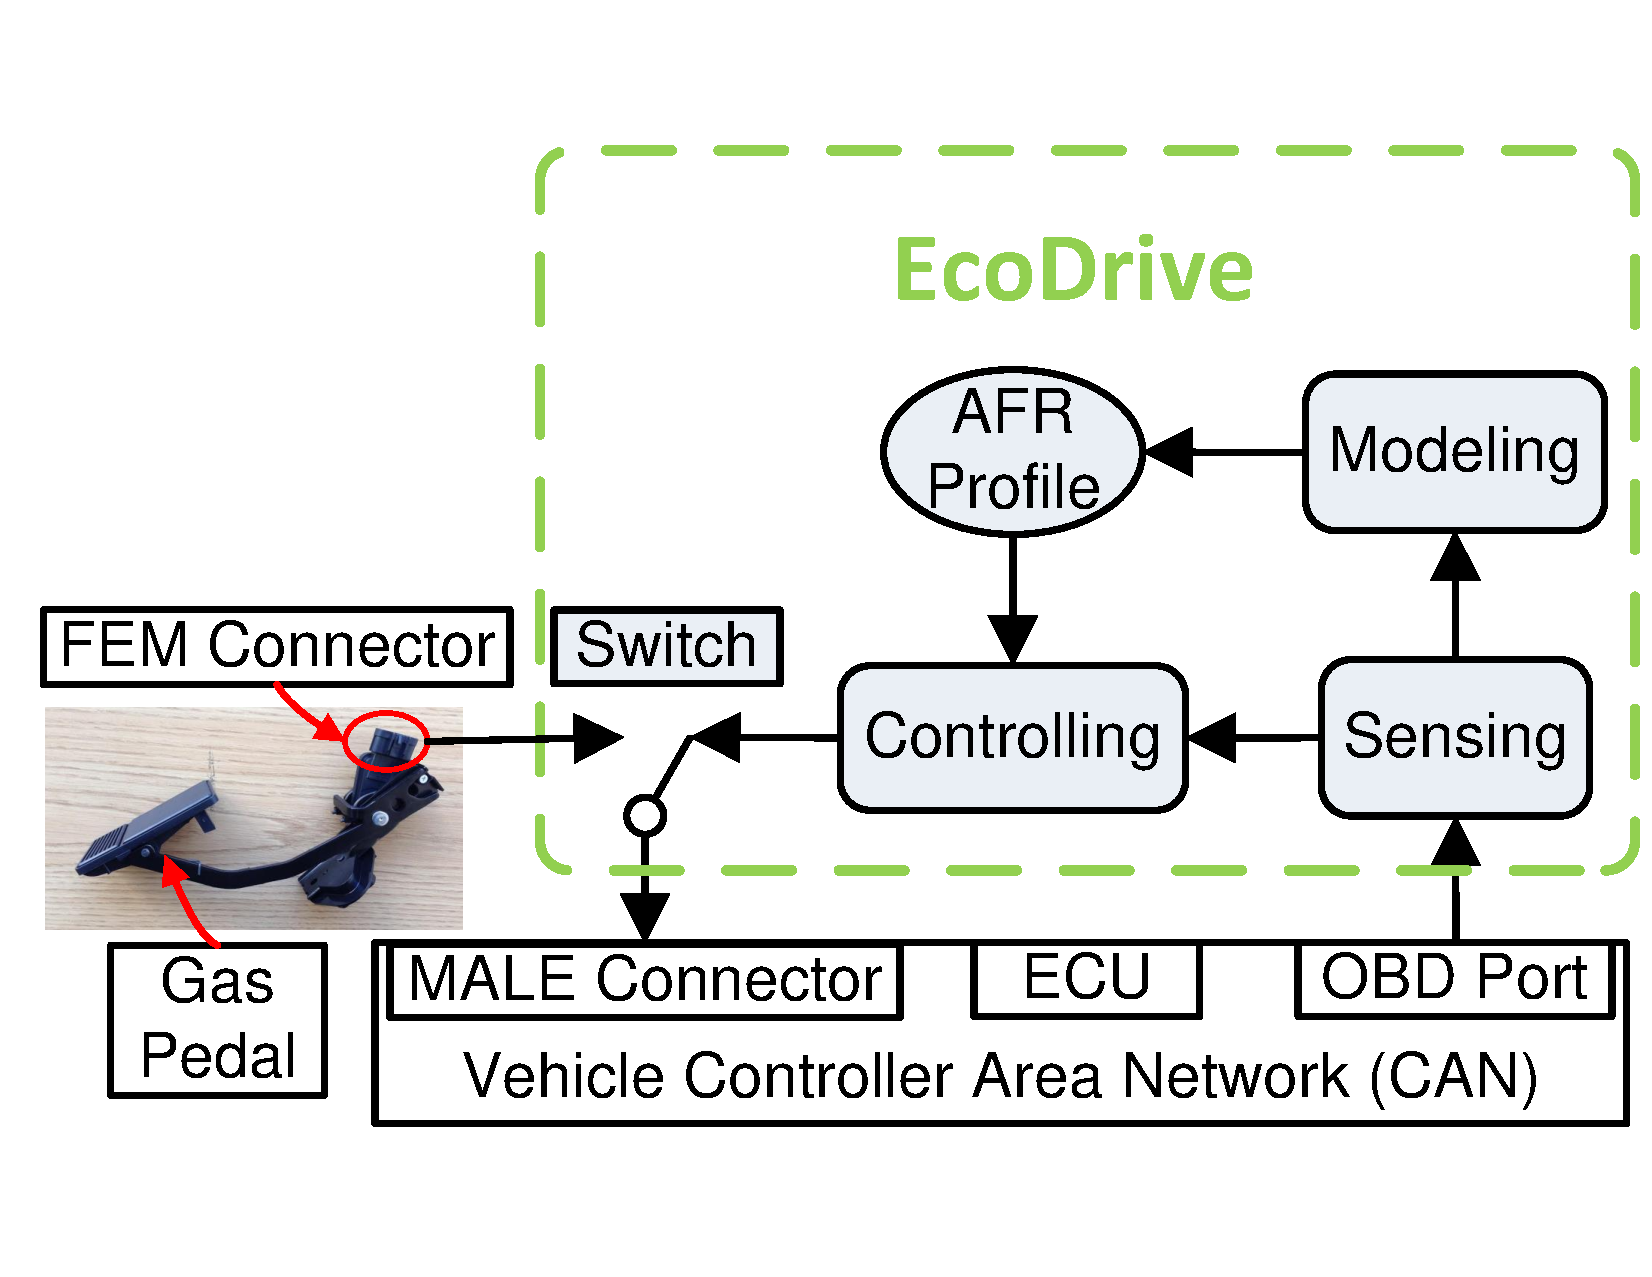
\includegraphics[width=4.0in,angle=0]{Figs/EcoDrive/architecture.pdf}
\vspace{-0.5cm}
\caption{EcoDrive Architecture.}
\vspace{-0.7cm}
\label{ecodrive}
\end{center}
\end{figure}


EcoDrive estimates instant fuel consumptions of different driving behaviors
based on sensed vehicle parameters from the On-board diagnostics (OBD) port \cite{obd, pid}. 
It can adjust vehicular speed in real time according to 
individual vehicle properties and road conditions 
to achieve higher fuel efficiency measured by Kilometer Per Liter (KPL)
\footnote{KPL refers to the distance travelled per unit volume of fuel consumed. 
It interchangeable with Mile Per Gallon (MPG), i.e., 1 KPL = 2.35214583 MPG.}.
EcoDrive is an independent system that can be installed on or removed from 
regular vehicles easily. 
This system controls the vehicle's acceleration and speed 
to provide a fuel efficient drive on its path. 
In our work and current implementation, 
we design this system assuming there is no other factors that 
would contribute to a choice of acceleration and speed, 
e.g., other vehicles, pedestrians, etc. or other obstacles in vicinity. 
Clearly in a practical system, this knowledge would be critical in modifying the acceleration behavior. 
Currently, we adopt the approach followed by other equivalent systems, 
such as cruise control \cite{cruise_control}, which allows the driver to instantly 
disable cruise control by actively pressing the brake pedal. 
In an analogous way, in our current implementation, 
we provide the driver a switch which can be pressed to instantly disable EcoDrive, 
if its acceleration behavior is perceived to be unsafe for nearby vehicles or obstacles.






\textbf{EcoDrive Components}. 
EcoDrive delivers its design via three components including an OBD sensing component, 
a vehicle dynamics modeling component and an acceleration controlling component. 
The architecture is illustrated in Fig. \ref{ecodrive}. 
The sensing component reads real-time OBD parameters through
the OBD port. 
The modeling component models various vehicle forces 
as functions of instant fuel consumption and produces
a fuel consumption profile, called Air/Fuel Rate (AFR) profile
\footnote{AFR refers to the volume of air/fuel cost per unit time.}.
The controlling component utilizes the AFR profile to calculate fuel efficient
driving strategies according to speed limit and road conditions. 
EcoDrive emulates the gas pedal by sending voltage values to 
the connector through an Arduino board.
The vehicular Electronic Control Unit (ECU) controls air/fuel injection rate
according to the voltage inputs. 

EcoDrive addresses two main challenges. 


%\textbf{How to model vehicle dynamics and build AFR profile by using OBD parameters, 
%given various vehicle types, transmission types and road conditions?}
\textbf{a) Model Vehicle Dynamics based on OBD Parameters}.
EcoDrive uses the OBD parameters delivered by
the sensing component to build an AFR profile, 
which records instant fuel consumptions of various accelerations under different speeds. 
To this end, EcoDrive models various vehicle forces, 
including propulsion, drivetrain loss, wind resistance
and grade resistance, as functions of instant fuel consumption.  
First, we model propulsion (or output torque) as a function of engine
torque and gear ratio \cite{vong2006prediction, giannelli2005heavy}. 
We use AFR to model engine torque, and use the ratio between RPM
and vehicular speed to model gear ratio. 
Second, we represent drivetrain loss and wind resistance as a function
of vehicular speed \cite{andersson2012online}.
The coefficients are estimated from recorded data traces where
the car is driving at constant speeds. 
The basic idea is that the sum of resistances is equal to
propulsion when the car is driving at a steady-state speed. 
Third, we model grade resistance by altitude changes over road segments. 
The altitudes of the locations are obtained from 
National Elevation Dataset \cite{nationalelevation}.   
Based on the three models, AFR is modeled as a function of 
speed, acceleration and road conditions. 


\textbf{b) Control Air/Fuel Rate and Vehicular Speed to Improve Fuel Efficiency}.
%\textbf{How to control accelerations and cruising speeds to improve
%gas mileage, given various road segment lengths and speed limits?}
EcoDrive controls vehicular speed by emulating gas pedal. 
It sends the emulated gas pedal position values to the
Arduino board which then converts the position
values to corresponding output voltages.
The output voltages are delivered to the ECU through a 6 Pin Connector.  
The problem is how to adjust vehicular speeds to travel through
a certain distance with the lowest fuel consumption.
We solve this problem by using dynamic programming. 
Each state of the dynamic programming model records 
the minimum air/fuel cost that allows the car to achieve
the current speed at the current location. 
In this model, speed can only increase and the last state of each
speed records the minimum fuel consumption if the car reaches the pre-assigned distance at that speed. 
We call the speed with minimum fuel consumption the target speed.  
By backtracking the state matrix from the last state
of target speed, EcoDrive can obtain the desired AFR at each speed. 
EcoDrive adjusts air/fuel injection rate based on real-time sensed vehicular speed. 
Once the vehicular speed reaches the target speed, EcoDrive
enters a cruising state and commands a constant air/fuel injection rate
until the car reaches the pre-assigned distance. 



\textbf{EcoDrive Prototype}. We build a prototype of EcoDrive in an off-the-shelf mobile embedded platform. 
The prototype is installed and tested on a 2011 Chevrolet Impala. 
We test EcoDrive on the Impala for more than 100 miles in both urban and highway environments.
We evaluate the fuel consumption of EcoDrive and human drivers on different road segments.   
In urban areas, EcoDrive achieves 10\%-40\% higher fuel efficiency than four recruited human drivers.
On highway, we evaluate EcoDrive on two highway segments with different target speeds.    
In our user tests, EcoDrive has over 30\% improvements compared to different human drivers. 
In comparison with cruise control, which is more fuel efficient
than human drivers in the traces we collected, 
EcoDrive achieves an average of 10\% higher fuel efficiency.  
We evaluate the performance of EcoDrive on other vehicles by using trace-driven simulation
based on the 10,000 miles data collected from 12 different vehicles. 
We further find that instant
fuel economy display on regular vehicles is misleading and cruise
control is fuel consuming during speed changes (either requested
by user or affected by road conditions).  






\section{RTDrive}


A self-driving vehicle is one that is capable of sensing 
its environment and navigating itself without human input \cite{wikiselfdrivingcar}. 
It uses a variety of techniques to sense its surroundings,
such as LIDAR, RADAR, odometry, and computer vision. 
It uses these different sensor inputs 
to understand its environment, 
recognize various road conditions, traffic lights, road signs,
lane boundaries, and track surrounding vehicles.
The potential benefits of self-driving vehicles
include increased safety, increased mobility and lower
costs. 
It is estimated that self-driving vehicles can reduce 90\%
of the accidents and prevent up to \$190 
billion in damages and health-costs annually
\cite{litman2014autonomous}.


Many commercial and academic endeavors are putting significant resources
for the development and tests
of such self-driving systems \cite{waymo, benz, autox}.
For example, Google started its self-driving project in 2009,  
and has spent more than \$1 billion
in building and testing fully self-driving vehicles~\cite{googlespend}. 
While legal and political challenges remain in its widespread adoption,
there are also some technical bottlenecks on the way of developing
completely reliable self-driving systems.


All self-driving systems make
decisions based on the perception of the environment and
predefined traffic rules. However, there has been occasional
failures of these systems when they have encountered scenarios
that were hitherto unseen. For instance, based on the situation
 in a construction
zone, human drivers would realize that it is permissible to cross
over a double yellow line by following the appropriately placed
cones  (which otherwise is illegal to cross
in the US), while a self-driving vehicle may not be able to
do so, and therefore be unable to move forward. Similarly in
poor weather conditions or due to traffic light malfunctions,  
the cues from different sensors may
contradict each other leading to confusion in decision making.

In general, the road rules are complex and may conflict with
each other, i.e., the system has to understand when
to follow cones and ignore lane markers, 
and when to obey a road worker and disobey traffic
signs.
%To address the last mile challenge, some recent work \cite{kang2018rc} 
%propose to use specially designated remote human operators
%to augment self-driving system when it fails to 
%perceive or handle current situations. 
While it is tempting to return control (during the failure of the self-driving
function) to a local human driver situated in the vehicle, 
it is foreseeable a future of driverless cabs carrying only
underage or licenseless passengers.
Hence, we expect that remote drivers can multiplex and manage
a large group of vehicles making scalability feasible.
However, accomplishing remote driving for a vehicle requires careful tuning 
of (wireless-based) network parameters, media content and their formats,
and control experience with some real-time constraints between the vehicle 
and the remote driving station.

%It is well established that human
%drivers, especially experts, are capable of making good judgement calls
%in face of contradictory or inadequate inputs, that sometimes limit 
%a learning system that has yet to encounter a scenario before.
%While it is tempting to return control (during the failure of the self-driving
%function) to a local human driver situated in the vehicle, 
%it is foreseeable a future of driverless cabs carrying only
%underage or licenseless passengers.
%Hence, we expect that remote drivers can multiplex and manage
%a large group of vehicles making scalability feasible.



In this paper, we present RTDrive, a remote driving framework
that augments self-driving system when it fails to 
percept and/or handle current situations. 
RTDrive consists of a live streaming system
and a remote control server. 
The live streaming system can encode videos by using
a context-aware video encoding algorithm. 
It also includes a live streaming protocol that 
carries out a consistent-latency
view mechanism to make the view of the operator
more smooth. 
The framework also consists of several modules, video codec, 
Forward Error Correction (FEC), vehicle dynamics sensing,
lane boundary detection, object detection etc.,
that enable further extension, optimization and innovation.  



\textbf{Context-Aware Video Encoding}.
The context-aware video encoding algorithm can 
sense vehicle dynamics and based on which it 
selects the optimal video encoding bitrate and key frame intervals. 
In video live streaming, the video is encoded into two
frames, I-frame and P-frame.
I-frame is also called key frame and it can be 
decoded into a complete image. 
P-frame only encodes the difference between current
frame to previous I-frames and P-frames. 
The context-aware video encoding algorithm
can dynamically adjust the number of I-frames
and P-frames to improve video encoding efficiency. 
The intuition is to adjust the key frame interval 
based on the frequency of camera view changes. 
For example, in the cases of turning or high speed scenarios,
there should be more I-frames since P-frames cannot
carry enough information which may lead to severe quality degradation. 
Through real world trip data collection and replay,
the context-aware video encoding algorithm can outperform
the default encoding algorithm by 10\%-30\% in various trips. 

\textbf{Live Streaming Protocol}.
We design and implement a live streaming protocol. 
It consists of several modules such as UDP/TCP, FEC, 
bandwidth and packet loss rate estimation. 
We discuss the design choices and evaluate these modules
under various network parameter settings. 
Also, a consistent-latency view algorithm 
is designed to deliver smooth
videos to improve the remote control experience. 
It uses a buffer to order the frames based on the timestamps
and deliver to the frame display engine only when it is 
the its order.
It achieves this goal by tracking two parameters, 
the latency difference and the latency deviation.   
The latency difference between
the live streaming system and the server is
tracked by using a low pass filter. 
The deviation of the latency difference is also recorded. 
Through a user study with 20 participates on controlling the Android-powered
vehicle, the operators with consistent-latency have
2x better control precision. 


This paper makes the following contributions:
\begin{itemize}
\setlength\itemsep{0em}

\item We design and implement RTDrive, a live streaming and remote control
framework, that can be used to view video stream and
control the vehicle remotely in real time. 
RTDrive can augment self-driving systems when they are
failed to percept the environment under various unpredictable conditions. 

\item We present a context-aware video encoding algorithm,
which can encode video frames according to vehicle dynamics. 
According to the traces we collected, it is able to improve
the video encoding efficiency by 10\% to 30\% on average in 
various driving scenarios. 

\item We propose a consistent-latency live streaming protocol,
which can adapt to wireless network conditions and buffer frames
for smooth display. 
It includes various modules such as bandwidth estimation, loss rate 
estimation, FEC encoding and frame buffering. 
According to a user study with 20 participates, 
the consistent-latency view algorithm improve the control
precision by more than 2x on average in a parking
task. 
\end{itemize}





\section{Contributions}


This thesis work makes the following contributions:
\begin{itemize}
\setlength\itemsep{0em}


\item We illustrate that the accuracy of smartphone built-in sensors are very sensitive
to road conditions and human interactions when conducting driving analytics. 
Traditional slope-unaware approach may caused misalignment and acceleration over/under
estimation, which may cause significant sensing errors. 
We develop several techniques to identify the usability and accuracy of inertial sensors 
and improve their performance.  
We consider using commodity mobile device GPS receivers to sense vehicle
motion parameters, especially those related to acceleration and brakes, 
and evaluate the performance by more than 
10,000 miles of driving data. 
We find that GPS can be a good candidate to estimate such vehicle
motions, especially in high speed scenarios (higher than $10m/s$ or $22mph$). 
It indicates that GPS can be a good alternative than inertial
sensors due to its simplicity and better performance in high speed
scenarios.  
We develop DriveSense, an Android application component that can 
selectively use GPS and inertial sensors for driving analytics. 
A beta version of DriveSense has been released to 9 volunteers and this version has
currently recorded more than 3,000 miles of driving data in the last six months.
Our evaluation shows that DriveSense can improve the overall performance 
comparing with using either GPS or well-tuned inertial sensors. 



\item We design and implement EcoDrive, 
which is an independent fuel consumption sensing and control system
that can improve fuel efficiency. 
The system is implemented on an embedded platform 
that can be easily installed on regular vehicles. 
We model various vehicle forces as functions of instant fuel consumption
and the models are evaluated by utilizing 
10,000 miles of driving traces collected from 12 vehicles. 
EcoDrive is installed on a regular vehicle and evaluated by more than 100 miles of driving in both urban and highway environments, 
and demonstrated to improve fuel efficiency compared to cruise control system
of the vehicle and to human drivers.  




\item We design and implement RTDrive, a live streaming and remote control
framework, that can be used to view video stream and
control the vehicle remotely in real time. 
RTDrive can augment self-driving systems when they are
failed to percept the environment under various unpredictable conditions. 
It includes a context-aware video encoding algorithm,
which can encode video frames according to vehicle dynamics. 
According to the traces we collected, it is able to improve
the video encoding efficiency by 10\% to 30\% on average in 
various driving scenarios. 
It also includes a consistent-latency live streaming protocol,
which can adapt to wireless network conditions and buffer frames
for smooth display. 
It includes various modules such as bandwidth estimation, loss rate 
estimation, FEC encoding and frame buffering. 
According to a user study with 20 participates, 
the consistent-latency view algorithm improve the control
precision by more than 2x on average in a parking
task. 




\end{itemize}






\section{Outline}

The rest of the thesis is organized as follows. 
In Chapter \ref{chapter_drivesense}, we present
our driving analytics system DriveSense, which leverages smartphone
sensors to monitor driving behaviors.
In Chapter \ref{chapter_ecodrive}, we present EcoDrive, an in-vehicle
system that can . 
In Chapter \ref{chapter_rtdrive}, we propose the live streaming
and remote control framework RTDrive, which can augment
self-driving systems upon occational failures. 
In Chapter \ref{chapter_relatedwork}, we compare our work with prior
approaches and systems to monitor, assist or even replace human
drivers. 
We conclude and discuss the avenues for further research in Chapter \ref{chapter_conclusion}.



                  % Chapter 1


\chapter{DriveSense: Practical Driving Analytics with Smartphone Sensors} 
\label{chapter_drivesense}

Sensing various driving behaviors, such as accelerations, brakes,
turns, and change lanes — is of great interest to many applications,
e.g., understanding drive quality, detecting road conditions, and
more. Many such applications rely on using smartphone placed in a
vehicle to collect such data for ease of deployment and use. However,
several driving analytics techniques in the recent past, including
our own, make simplifying assumptions that the smartphone is
stably fixed with certain orientation and the car is driving on flat
roads. Our deployment experience reveals that existing approaches
may cause orientation misalignment and acceleration over/under
estimation due to road slopes and human interactions, which lead
to significant sensing errors for driving analytics applications.
In this chapter, we present a smartphone app called DriveSense,
which addresses these challenges and conduct driving analytics
accurately by using various smartphone sensors.  


\section{The Problems}


Smartphone inertial sensors are used for driving analytics. 
The IMU accelerometer measures 3D acceleration 
\footnote{Depending on context, acceleration refers to either the 
rate of change of velocity per unit of time or the driving behavior
when the driver press the gas pedal.} 
changes and can be used to detect accelerations and brakes. 
The IMU gyroscope measures 3D angular change and can be used
to detect steering motions such as turns and lane changes.
Existing driving analytics approaches \cite{wang2013sensing,hansenspeed,chen2015invisible} 
assume ideal scenarios, i.e., 
the car is moving on flat road and  
the smartphone is stably mounted
with fixed relative orientation to the car. 


In trying to relax such assumptions, 
we found that the accuracy of inertial sensors, 
especially the accelerometer, are sensitive to road conditions, 
orientation changes and mounting stability (as a result of human interactions). 
We start with an example trip to illustrate the 
\emph{acceleration over/under estimation} problem
due to slopes and the effects of gravitation.  
We show that existing coordinate alignment
method may cause \emph{coordinate misalignment}. 
Such problems cannot be easily fixed due to 
the low accuracy of inertial sensors. 
We also discuss unmanaged smartphone usage
cases and the impacts on driving analytics, 
i.e., relative orientation changes and the 
smartphone is not stably mounted. 

\subsection{Sensitive to Road Conditions}

\subsubsection{Acceleration Over/Under Estimation}


\begin{figure}[!tbp] \centering
    \begin{subfigure}[b]{\linewidth}
         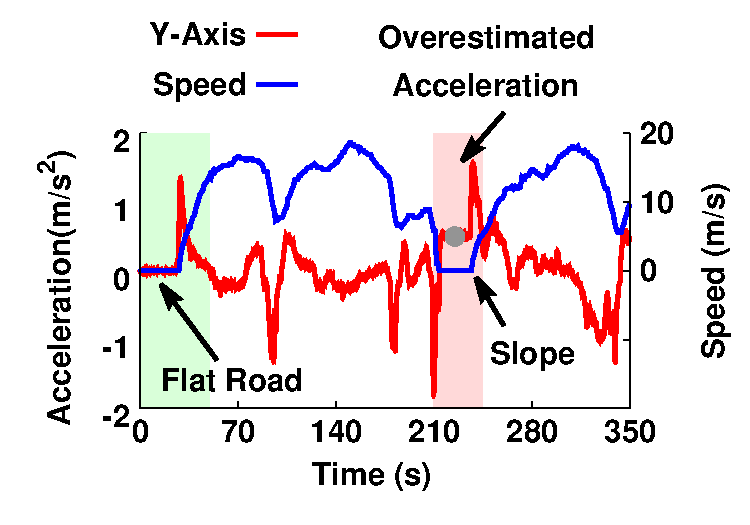
\includegraphics[width=3.3in,angle=0]{Figs/DriveSense/slopeaware/motivation.pdf}
         \vspace{-0.4cm}
         \caption{The accelerometer y-axis (along the car's heading direction) and OBD speed readings.}         
        \label{motivation:a}
    \end{subfigure} %

    \begin{subfigure}[b]{\linewidth}    
        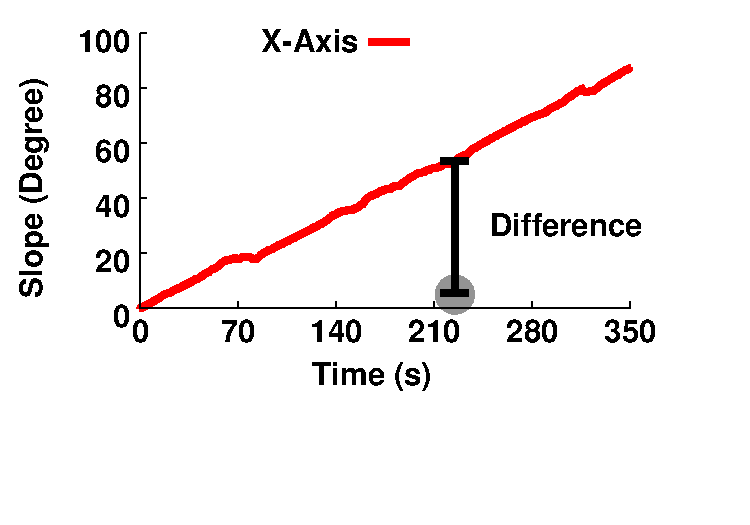
\includegraphics[width=3.3in,angle=0]{Figs/DriveSense/slopeaware/gyro_motivation.pdf}
        \vspace{-1.5cm}
        \caption{The accumulated gyroscope x-axis (tracking car's rotational speed when going upslope/downslope) readings.}
        \label{motivation:b}    
    \end{subfigure} 
\caption{Sensor and OBD data from the motivation example trip.}
\label{motivation}
\vspace{-0.2cm}
\end{figure}



We collect an example driving trip with various driving activities 
such as brakes and accelerations using a LG Nexus 5.
Before the trip, we park the car in a flat parking lot and fix
the smartphone with a frame mounted between the driver seat
and the passenger seat.
The coordinates of the phone are manually aligned (as precisely as we can) with the car. 
We use a customized Android application to record the sensor data and OBD speed data.
The sensor and OBD data traces of the trip are illustrated in Fig. \ref{motivation}.
As can be seen from the figure, the trip started on a flat road
and the speed was $0m/s$ with acceleration $0m/s^2$. 
At time $210s$, there is a stop as the OBD speed reading was $0m/s$ 
while the accelerometer reading is around $0.5m/s^2$ indicating
the car is accelerating. It is an overestimated acceleration
due to road slope.
This is because the y-axis of the accelerometer can sense the gravity. 
The gravitational force may have an incremental or decremental effect
on the estimation of vehicle motion parameters. 
For example, a misalignment of five degrees may cause $0.85m/s^2$ 
acceleration estimation error.
For reference, the \emph{Snapshot Program} \cite{snapshot} records a hard brake if the deceleration is around $3m/s^2$.
Therefore, we conclude that \emph{road slopes and associated gravitational effect
cause acceleration over/under estimation}. 


\subsubsection{Accumulated Gyroscope Errors}

The gyroscope can be used to track three-dimensional angular changes
and is an ideal input for slope estimation. 
However, it is known to suffer accumulated errors \cite{zhou2014use}. 
As illustrate in Fig. \ref{motivation}, 
we observe similar error accumulation in our motivation experiment. 
The dark dot is the slope gradient calculated by the accelerometer.
The curve of gyroscope measures the accumulated angular changes  
when the car was driving upslope/downslope.
Intuitively, the accumulated angular change of gyroscope can be used to 
estimate the slope gradients.
Clearly, the accumulated error is much higher than 
the actual accumulated slope gradients estimated by the accelerometer. 
We refer interested readers to \cite{chen2015invisible, zhou2014use},  
for detailed gyroscope three-dimensional readings 
and corresponding vehicle movement. 
Since we only focus on going upslope/downslope, we are interested in 
x-axis gyroscope readings of the car (or aligned smartphone) only.
There are several reasons why we see accumulated errors of gyroscope. 
The first one is the constant drifts, where the gyroscope reading is 
not zero in still due to limited hardware precision.
As the angular changes add up, the constant drifts accumulate correspondingly, 
which leads to a rough linear function between accumulated error and time.
The second one is the vibration of the vehicle, which accelerates
the drifts of the gyroscope readings.
Misalignment (caused by either manual alignment in our experiment 
or the coordinate alignment algorithm) between the car and the smartphone can also introduce accumulated errors. 
This is because the x-axis of the gyroscope can also sense car's steering angular change like turns and lane changes
when the smartphone is misaligned with the car.

\subsubsection{Coordinate Misalignment}

\begin{figure}[!htbp]
\begin{center}
  \vspace{-0.2cm}
  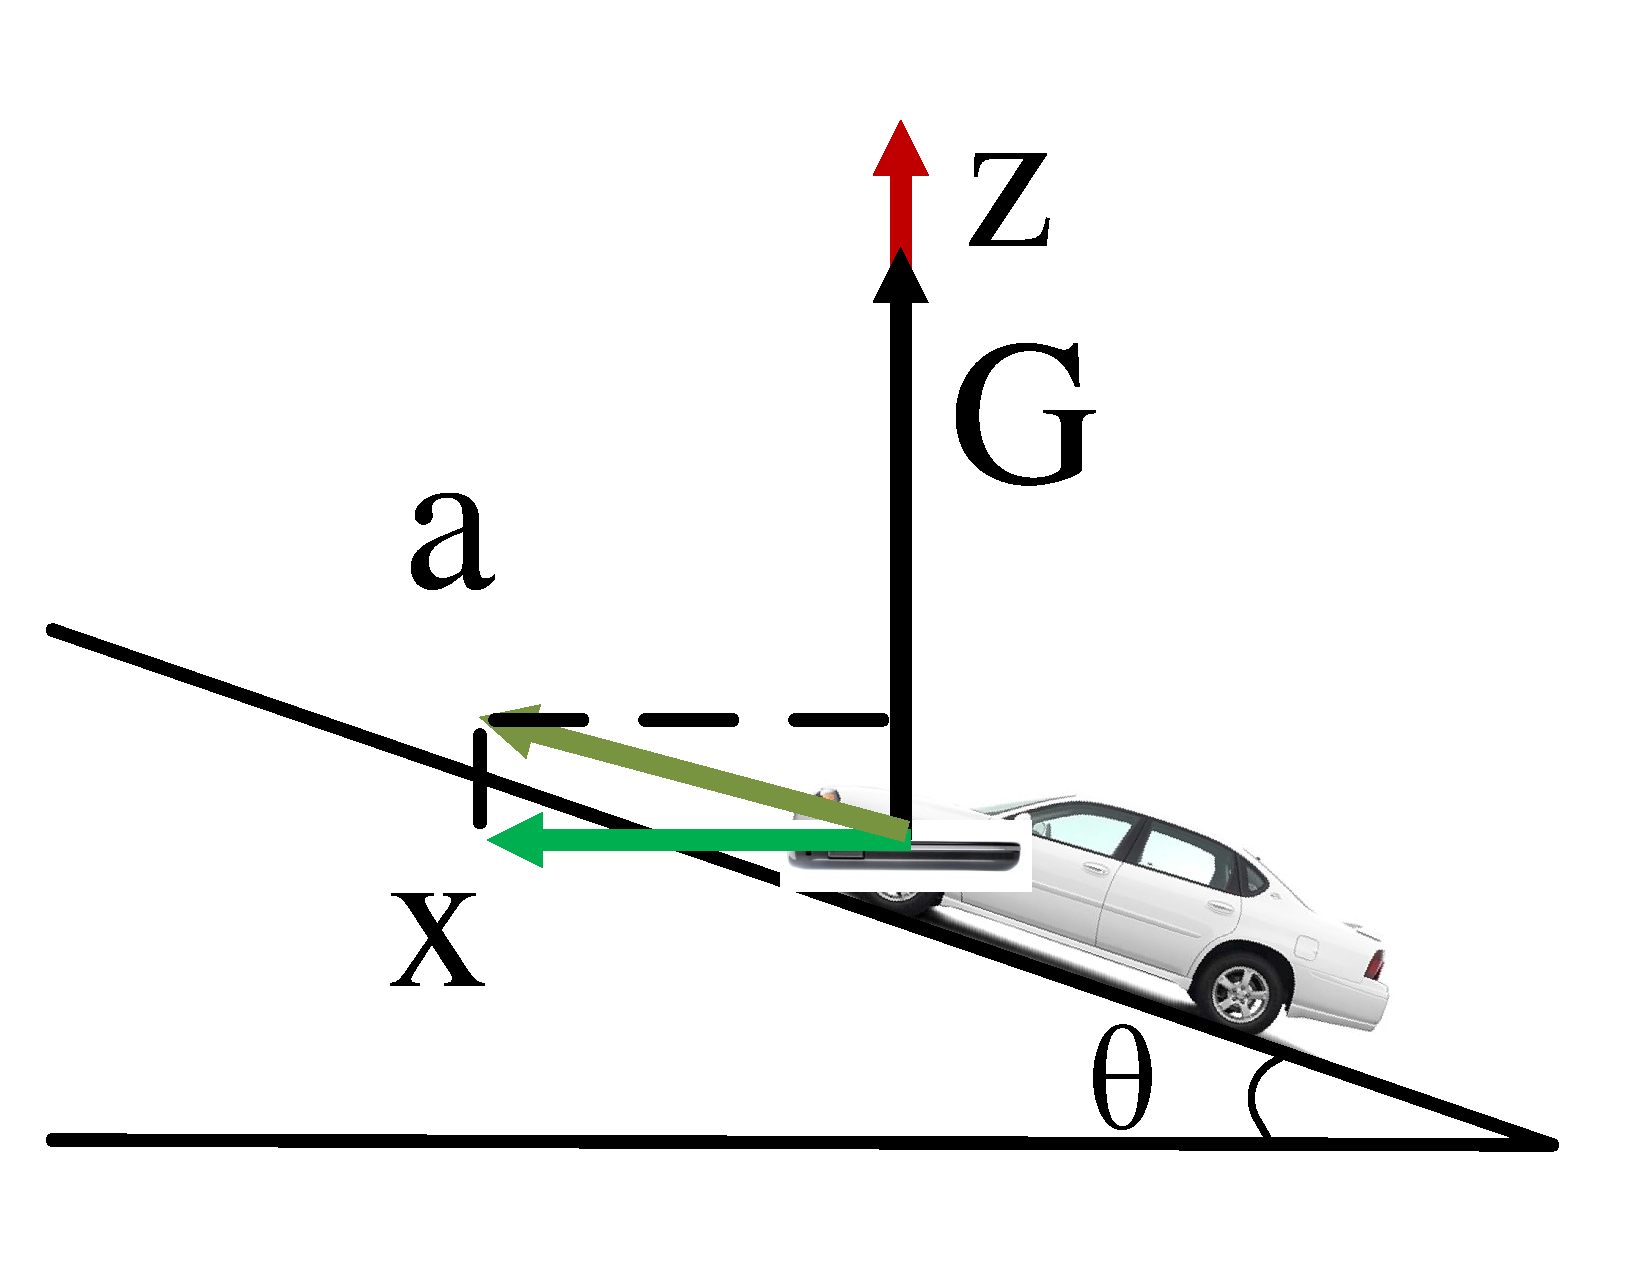
\includegraphics[width=2.6in, angle=0]{Figs/DriveSense/slopeaware/misalignment.pdf}
\vspace{-0.2cm}
\caption{Coordinate misalignment caused by road slopes.}
  \label{slopemisalignment}
\vspace{-0.4cm}
\end{center}
\end{figure}

Coordinate alignment is the process to align the
coordinates of the smartphone to those of the car 
\cite{hansenspeed, wang2013sensing, chen2015invisible}. 
We find that slopes cause misalignment
if the coordinate alignment is conducted on slope. 
Coordinate misalignment refers to the case when the aligned coordinates of 
the smartphone is not perfectly aligned with the coordinates of the car. 
Since the accelerometer can sense gravity, a misalignment
may also cause acceleration over/under estimation problem. 
As illustrated in Fig. \ref{slopemisalignment}, 
the car is moving upslope while the coordinate alignment algorithm
assumes the car is moving on flat road, 
which leads to the intersection angle $\theta$ between
aligned coordinates of the smartphone and the coordinates
of the car. 
Such misalignment may cause acceleration over/under estimation
when the driver is driving on flat road. 


\subsection{Sensitive to Human Interactions}


Human interactions may change the 
relative orientation and mounting stability of the smartphone, 
which degrade the usability and accuracy
of inertial sensors. 
Relative orientation change refers to the
orientation change of the smartphone independent of
the movement of the car. 
Imaging a passenger pick up the phone from pocket
and answer a phone call, 
the movement of the smartphone is the addition of 
the movement caused by human interactions and vehicle movements. 
Mounting stability refers to the degree of fixation of the smartphone, 
i.e., the mounting stability when the smartphone is fixed in car mount
it higher than the case when the smartphone is put in the pocket. 


The relative orientation change causes the sensor
readings are too noisy to be used.
Suppose the smartphone is rotated horizontally 
180 degree, then the output of accleleromter 
is completely reversed, i.e., the smartphone
detects brake when the car is accelerating. 
To eliminate such errors, 
the rotation matrix should be
re-estimated for accurate output. 
Coordinate alignment is an expensive process, 
which we will discuss in details in later sections, 
and frequent coordinate alignment may lead to 
gray period where the inertial sensors
cannot used for driving analytics. 



Mounting stability is also an important factor when 
conducting driving analytics by using inertial sensors. 
When the user puts
the smartphone in the pocket,
the vibration of smartphone may add extra noises.
We advocate the use of a metric to quantify mounting stability
and understand the sensor accuracy under
various stability levels. 




\section{Sensing with Inertial Sensors}
\label{imusensors}


IMU sensors are used in many driving analytics 
applications \cite{hansenspeed, wang2013sensing, chen2015invisible}. 
However, existing work assume the car is moving on flat 
roads and the smartphone is stably mounted in the vehicle. 
Different from these work, we propose several novel
techniques to improve the accuracy and usability of inertial sensors
by detecting orientation change, modeling stability,  
conducting slope-aware coordinate alignment and linear
acceleration estimation in a more practical manner. 
We design a slope-aware solutions to conduct 
coordinate alignment and track linear acceleration
by removing the gravity component dynamically from the aligned accelerometer readings. 
Second, we use clustering techniques to detect 
relative orientation changes. 
Third, we use moving variance to model the mounting
stability of the smartphone and evaluate sensing accruacy
based on mounting statiblity. 

\subsection{Slope-Aware Alignment}
\label{slopeaware}


\begin{figure}[!tbph]
\vspace{0.0cm}
\hspace{-0.5cm}
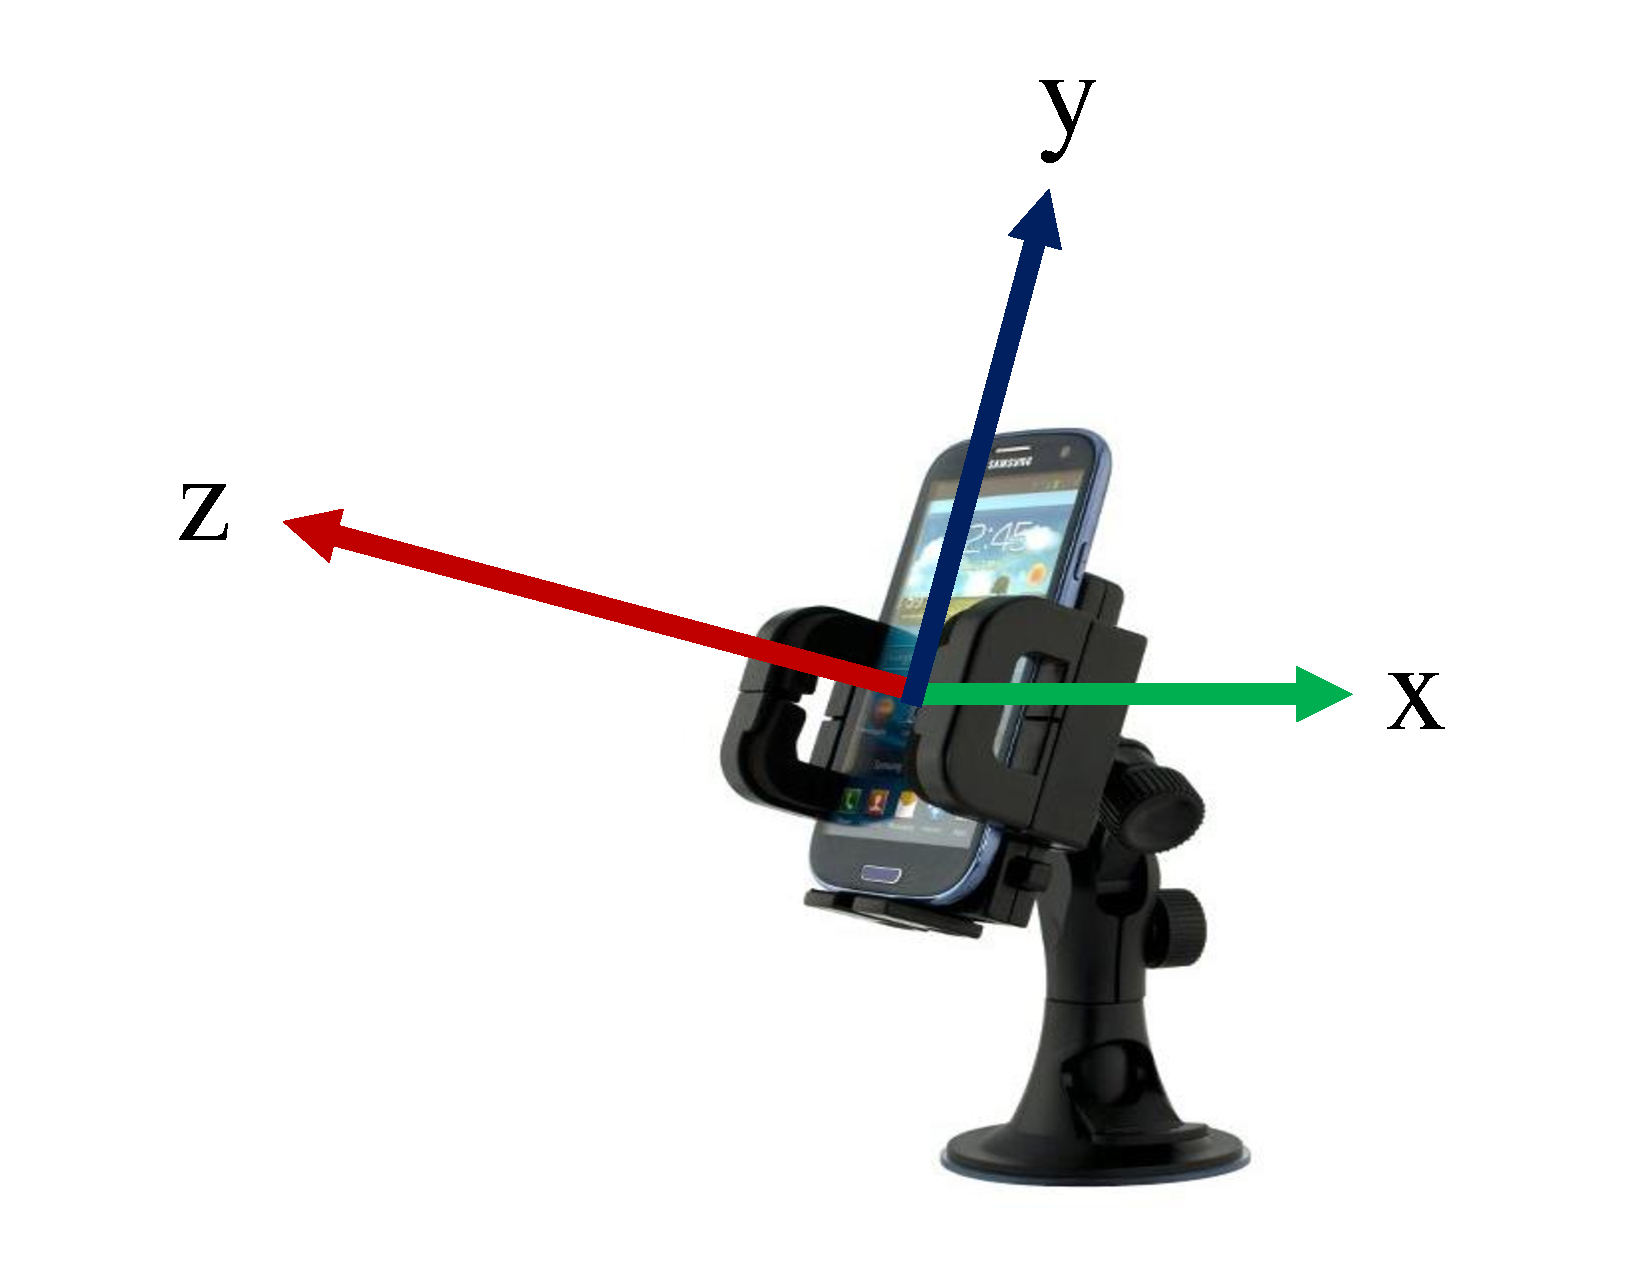
\includegraphics[width=1.8in,angle=0]{Figs/DriveSense/phone3d.pdf}
\vspace{0.0cm}
\hspace{-1.0cm}
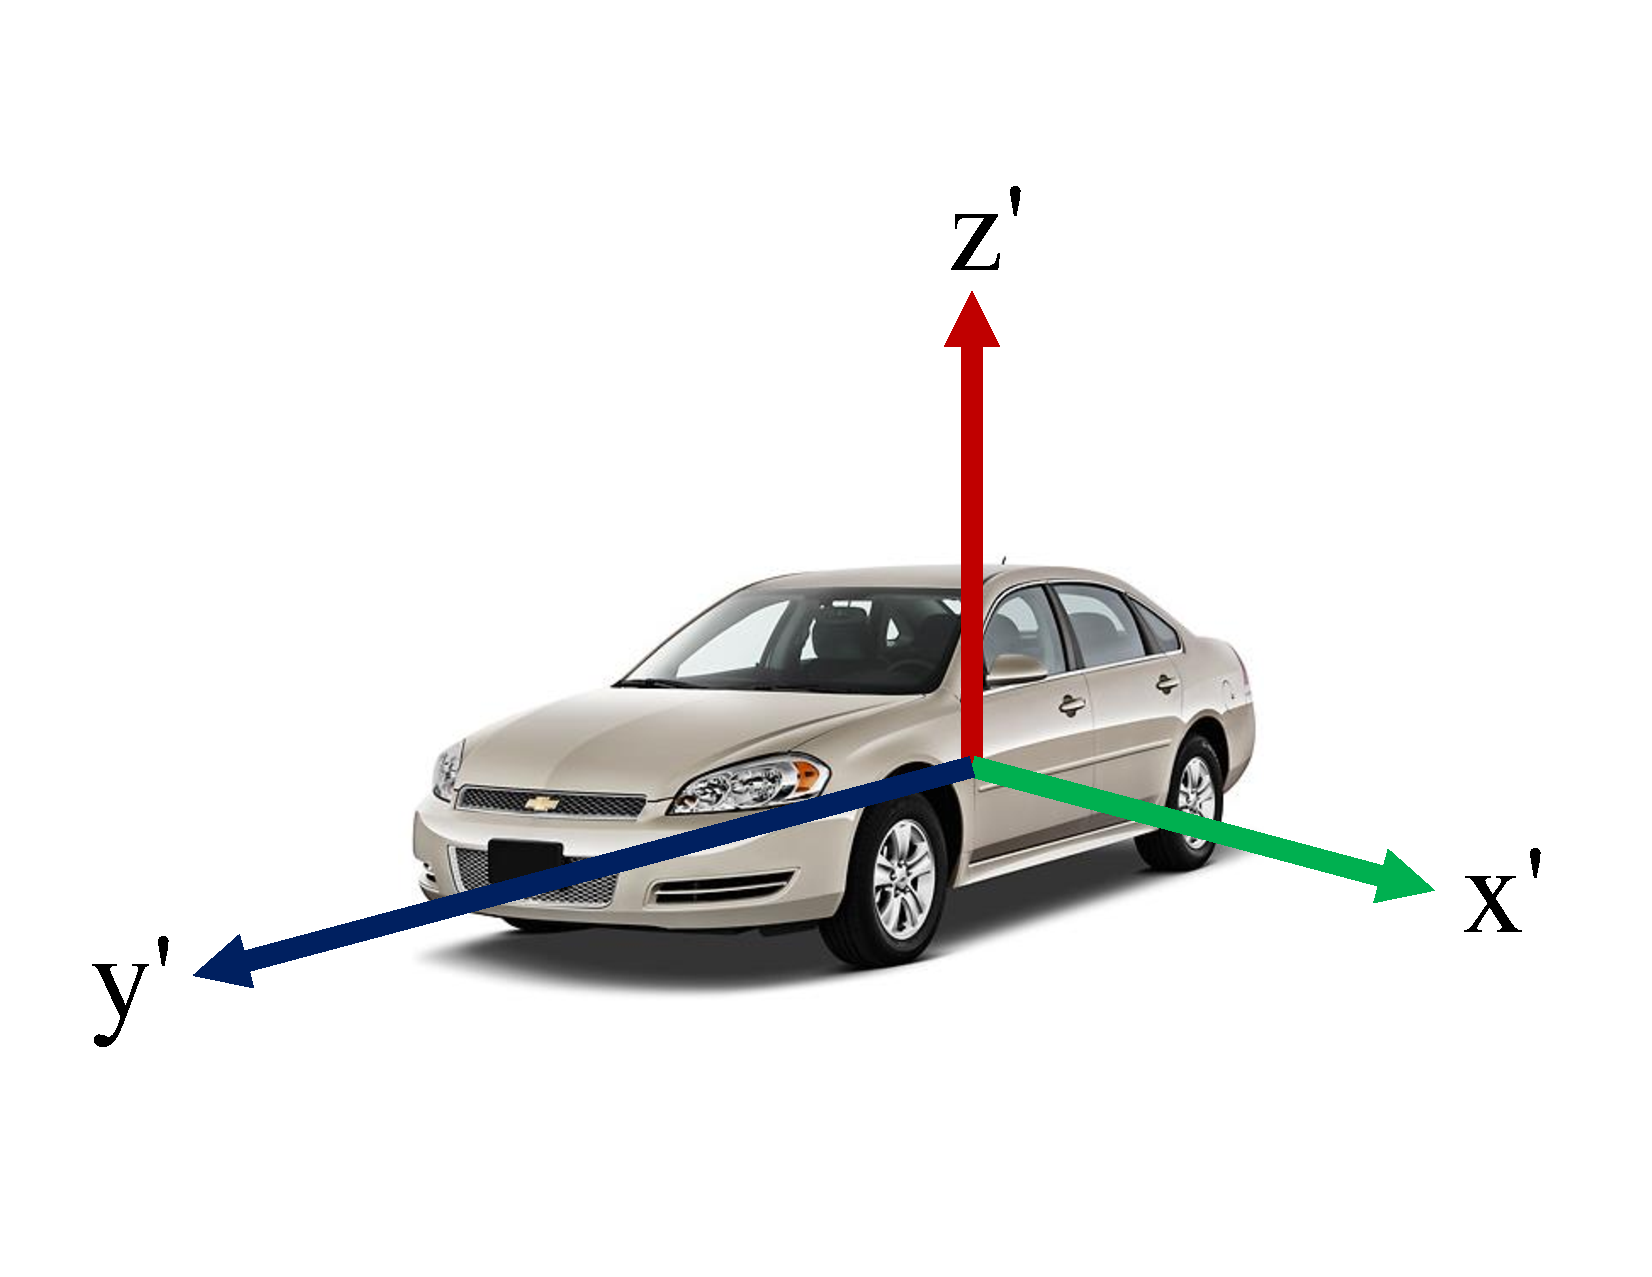
\includegraphics[width=1.8in,angle=0]{Figs/DriveSense/car3d.pdf}
\vspace{-0.2cm}
\caption{Coordinate system difference between a smartphone $[x, y, z]$ and a car $[x', y', z']$.}
\vspace{0.2cm}
\label{coordinates}
\end{figure}


\subsubsection{Slope-Aware Alignment and Linear Acceleration Estimation}


As illustrated in Fig. \ref{coordinates}, we use 
$[x, y, z]$ to represent the three dimensions of a smartphone
and use $[x', y', z']$ to represent the three dimensions
of a car. 
Coordinate alignment is the process that trains the rotation
matrix $R = [\hat{i}, \hat{j}, \hat{k}]$, 
where $\hat{i}$, $\hat{j}$ and $\hat{k}$ are three unit coordinate vectors,
so that $[x', y', z'] = [x, y, z] \times [\hat{i}, \hat{j}, \hat{k}]$.




\textbf{Step 1: Stop Points Extraction}. 

Identifying stop points are useful to conduct an initial alignment. 
We use a sliding window to track the deviation of the
accelerometer readings for this purpose.
The deviation is expected to be small when the car is stopped, 
i.e., in front of stop sign of red traffic light. 
But different cars have different vibrations, 
which affect the readings of the accelerometer. 
To identify a threshold for the deviation, 
we extract the stop points according to the speed information
collected from the OBD port.
We record the start time $s_t$ and end time $e_t$ that 
any speed reading in between is zero. 
To eliminate possible asynchronization and drifted value
after passing low-pass filter, 
we remove the points of the first 500ms and the last 500ms,
i.e., the data points within $[s_t + 500, e_t - 500]$. 
This process helps us to set the threshold to detect
stops. 
We only use OBD as a training input, 
our method can be used on any smartphone and vehicle settings
without OBD inputs. 
 

\textbf{Step 2: Horizontal Alignment}. 


Road slope affects the accuracy of coordinate alignment
in each step. 
During horizontal alignment, a slope-aware alignment method can
be much more effective than a slope-unaware approach. 
As illustrated in Fig. \ref{direction}, 
slope-unaware solutions assume all the data points 
pass the origin point and try to fit all the data
points for a single fit curve, 
while slope-aware solution treats each road segment
as different inputs (deviating from the origin point
due to slopes) and combine to improve the accuracy. 

To train the rotation matrix, we need to select the segments that the car is moving 
straight, and estimate the angle between the 
heading direction and the smartphone's horizontal coordinates \cite{wang2013sensing}.
To derive the rotation matrix from discrete sensor data points, 
we need to fit the curve and find the direction unit vector. 
We propose to train the horizontal
unit vector for each segment and combine each training results gradually with different weights.
There are lots of straight driving segments as illustrated in Fig. \ref{direction}, 
but not all of the segments are good for the training purpose. 
Each segment is selected based on the number of data points that
indicate the car is moving.
The intuition is that more data points could be more statistical significant. 
In Fig. \ref{direction}, we separate four segments and train the 
horizontal unit vector separately.
Clearly, this approach gives better view results that the four slopes of the 
fitting curves are $-0.98$, $-0.87$, $-0.93$ and $-0.95$, respectively. 
The weighted average is $-0.94$. 
After obtain the angle $a$, the horizontal 
rotation matrix can be calculated as follows. 

\[
R_h
	=
\begin{bmatrix}
   cos(\alpha) & -sin(\alpha) & 0 \\
   sin(\alpha) & cos(\alpha) & 0 \\
   0 & 0 & 1
\end{bmatrix}
\]



\begin{figure}[!tbph] 
\hspace{-0.4cm}
  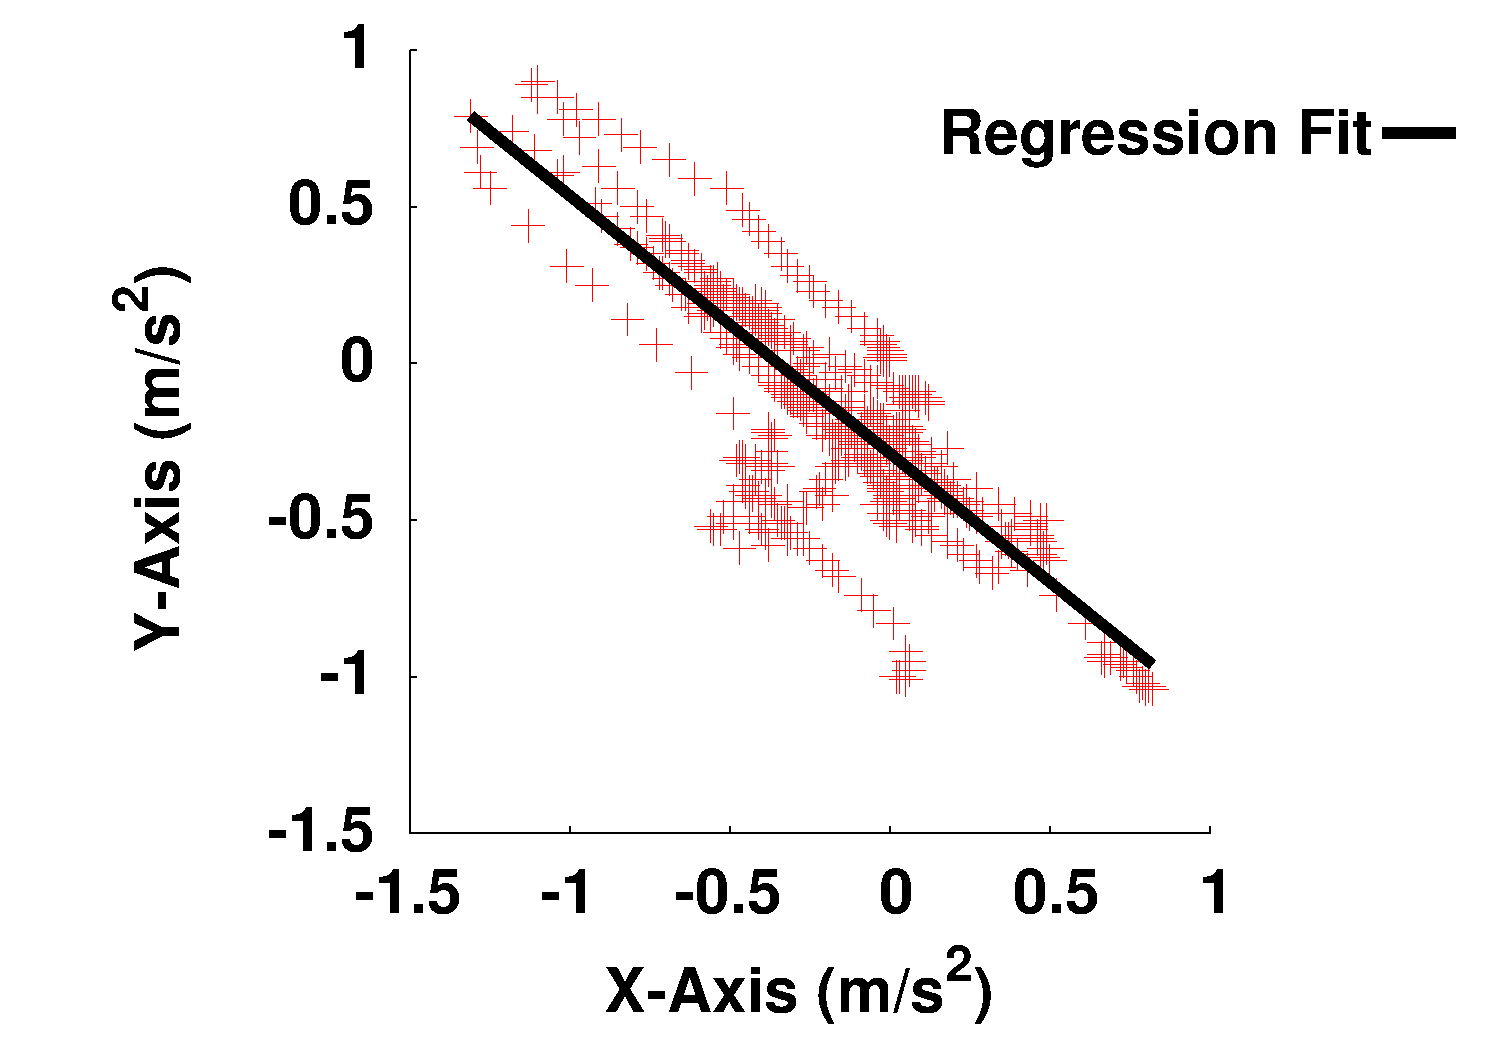
\includegraphics[width=2.6in,angle=0]{Figs/DriveSense/slopeaware/stateoftheart.pdf}
\hspace{-0.0cm}
  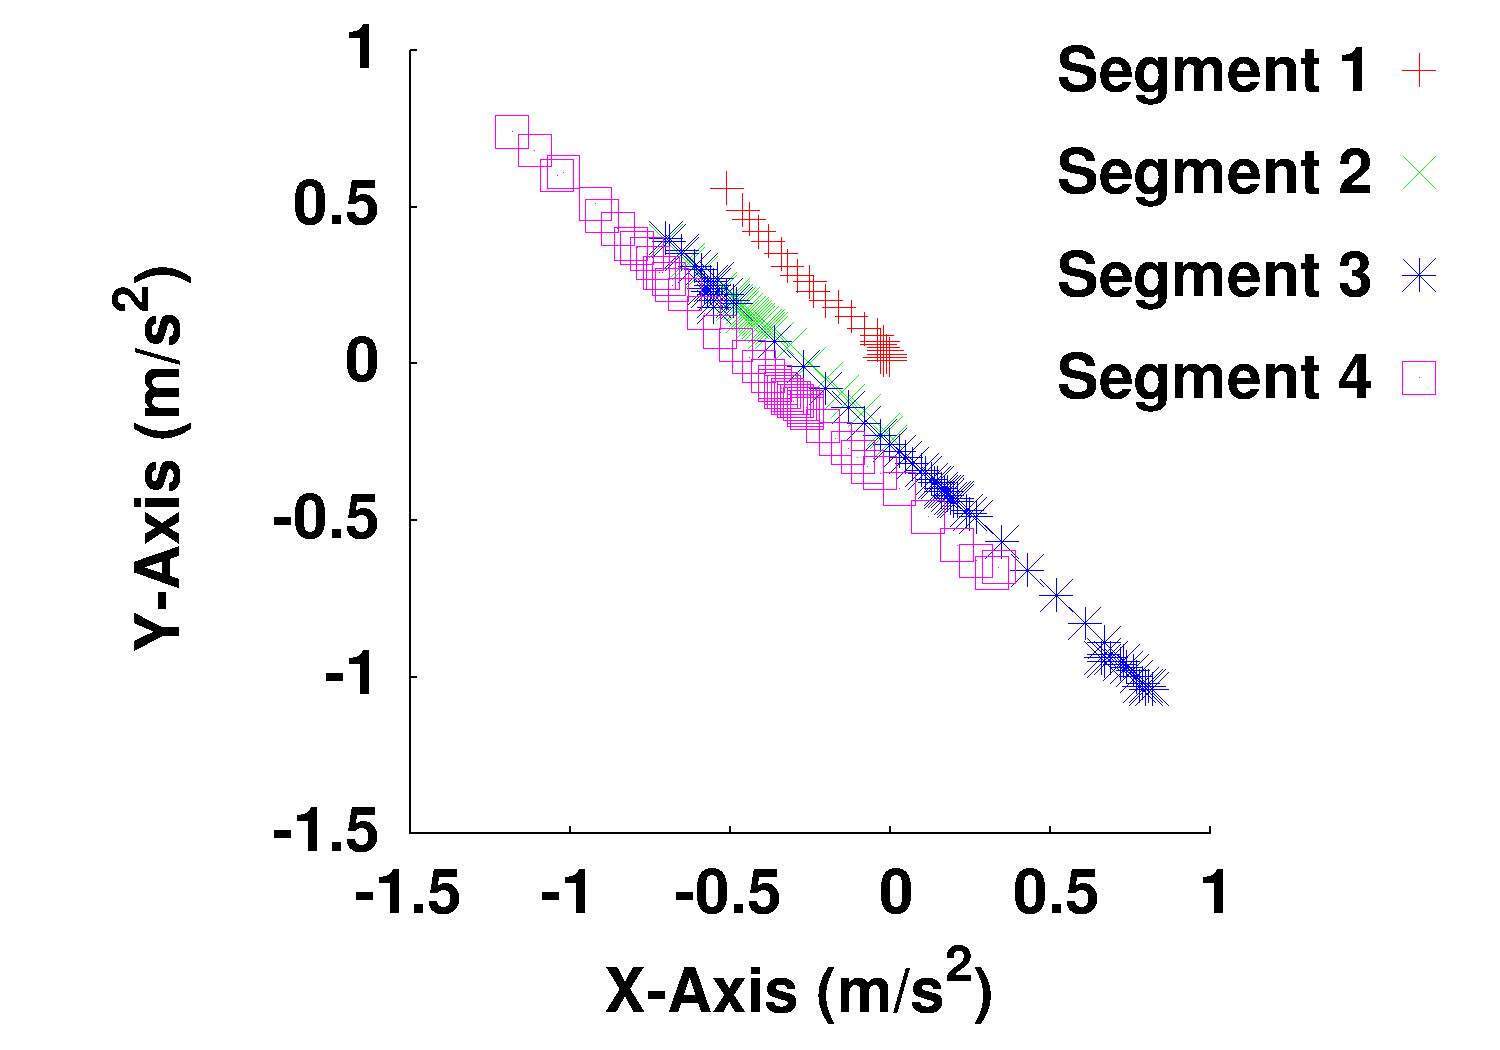
\includegraphics[width=2.6in,angle=0]{Figs/DriveSense/slopeaware/direction.pdf}
\hspace{-0.0cm}
   \caption{Training horizontal rotation matrix by using traditional
approach (above) and slope-aware multi-segment method (below).}
\label{direction}
\vspace{0.4cm}
\end{figure}





\begin{figure}[!htbp]
\begin{center}
%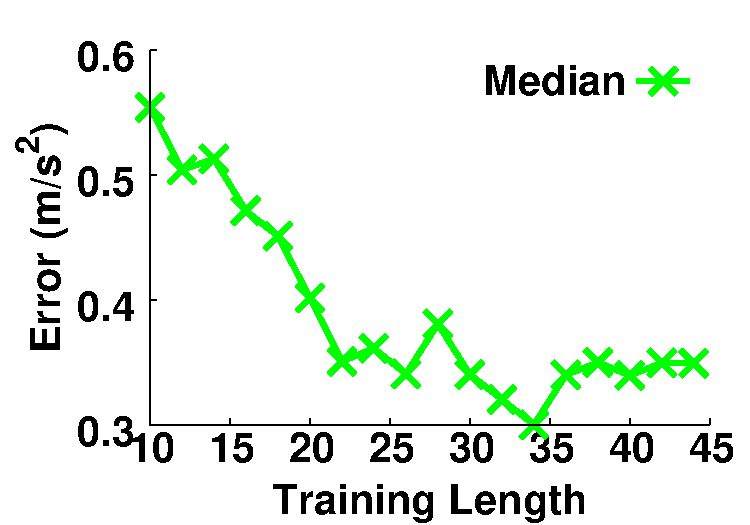
\includegraphics[width=1.7in,angle=0]{Figs/DriveSense/trainlengthanderror.pdf}
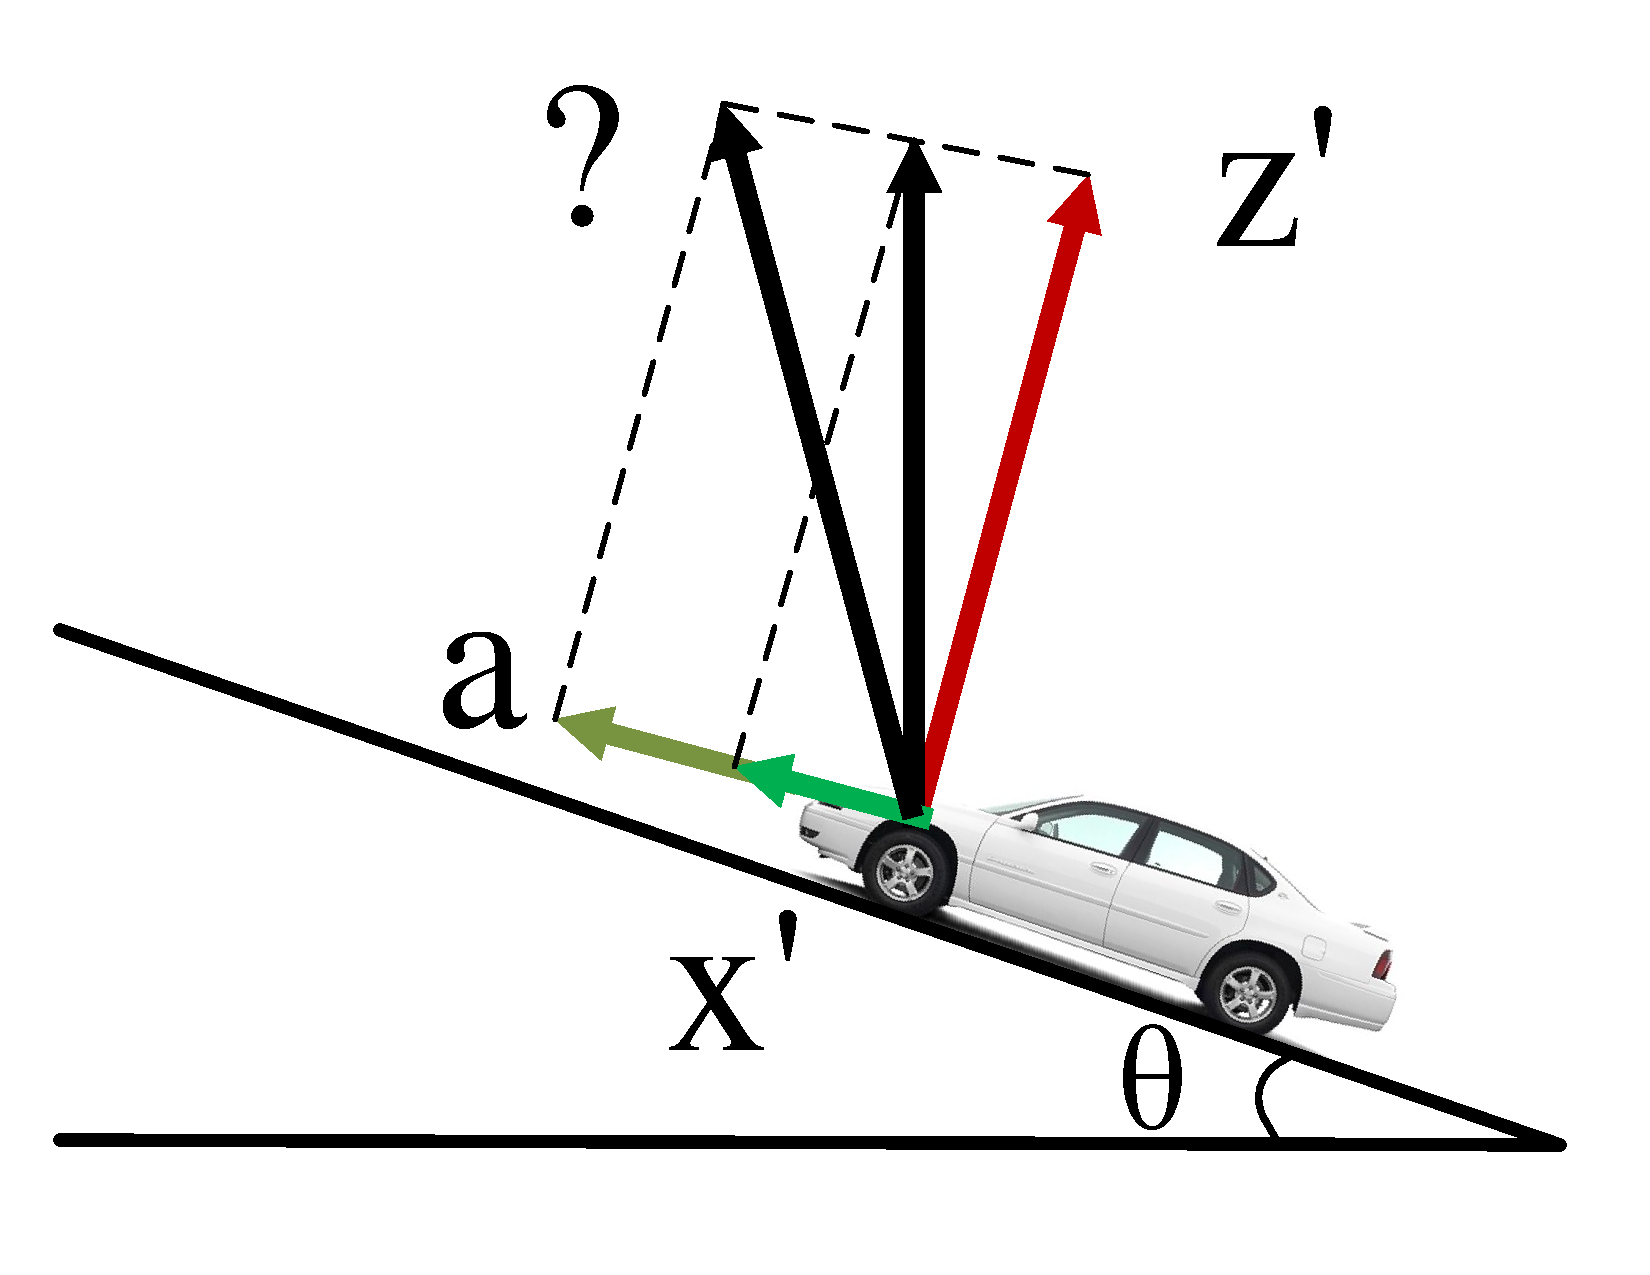
\includegraphics[width=2.0in, angle=0]{Figs/DriveSense/uncertain_vertical.pdf}
\vspace{0.0cm}
	\caption{
Since the actual acceleration of the car 
and the component of gravitational force (along the slope) are unknown, 
the direction of force is uncertain when conducting vertical alignment.
}
\label{training}
\vspace{0.4cm}
\end{center}
\end{figure}



\begin{algorithm}
\caption{Angle Search Algorithm}
\label{search}
\begin{algorithmic}[1]
\Input{$D_a$: The 2D accelerometer data after horizontal alignment}
\Output{$\theta_{o}$: The best fit angle}
\Procedure{AngleSearch}{}
\State $dev_{min} \gets MAX$;
\State $D_{t} \gets []$;
\For{$\theta$ \texttt{in} (-$\alpha$, $\alpha$)}
\For{$[y_i, z_i]$ \texttt{in} $D_a$}
\State $M_\nu$ $\gets$ $\begin{bmatrix}\cos\theta & -\sin\theta\ \\ \sin\theta & \cos\theta \end{bmatrix}$;
\State $[y'_i,z'_i]$ $\gets$ $[y_i,z_i]* M_\nu$;
\State $D_t.push(z'_i)$;
\EndFor
\State $dev_x \gets deviation(D_t)$;
\If {$dev_x < dev_{min}$}
\State {$dev_{min}$ $\gets$ $dev_x$};
\State {$\theta_{o}$ $\gets$ $\theta$};
\EndIf
\EndFor
\Return $\theta_{o}$;
\EndProcedure
\end{algorithmic}
\end{algorithm}
\vspace{-0.6cm}


\textbf{Step 3: Slope-Aware Alignment}. 

Estimating road slope at alignment time is challenging. 
In horizontal alignment, we can fit a curve as the moving
direction of the car (or the direction of force) is fixed and not much interfered 
by gravity. 
In vertical alignment, however, the direction of force is changing. 
As illustrated in Fig. \ref{training}, the direction of force changes
as the change of the acceleration of the car. 
There are two parameters are unknown, the slope gradient 
and the vehicle acceleration. 
The vehicle acceleration varies at each data point, 
which varies the direction of force and makes it is very
challenging to estimate the parameters.
We use one heuristic searching algorithm to search for best alignment angle. 
The algorithm relies on the property that the $z'-axis$ of 
the car should be constant over the same slope. 
Firstly, we assume the horizontal alignment is complete and
we convert a 3D alignment problem into a 2D alignment problem. 
The two dimensions are $y-axis$ and $z-axis$, 
as illustrated in Fig. \ref{training}.
By iterating over all the possible angles, 
we calculate deviation of the $z'-axis$ and locate the one with the least deviation. 
The pseudo code of the search algorithm is illustrated in 
Form \ref{search}.




\textbf{Step 4: Linear Acceleration Estimation}.



\begin{figure*}[t]
\begin{center}
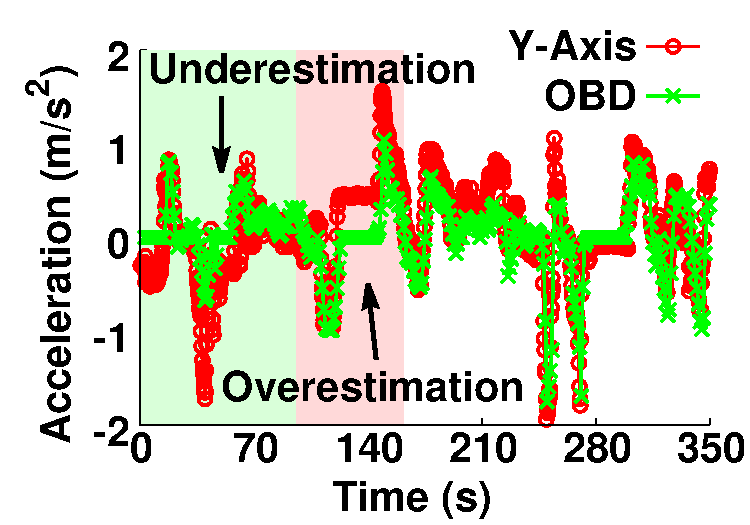
\includegraphics[width=2.2in,angle=0]{Figs/DriveSense/slopeaware/accspeed.pdf}
\hspace{-0.0cm}
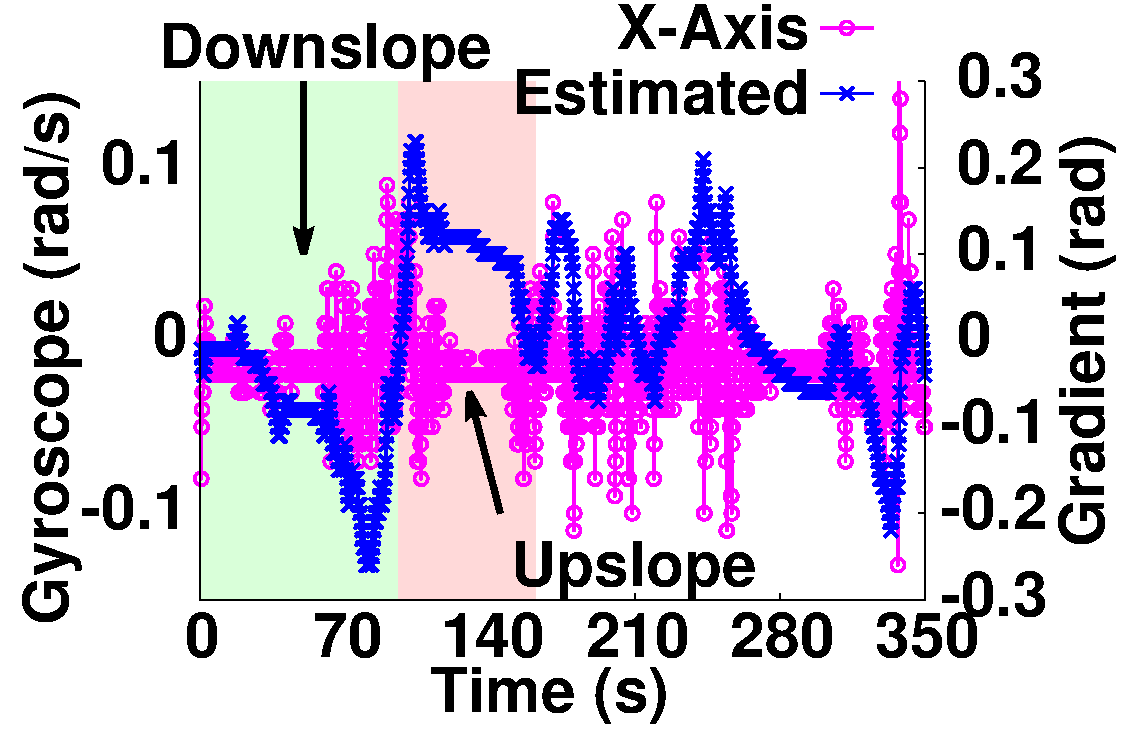
\includegraphics[width=2.2in,angle=0]{Figs/DriveSense/slopeaware/gyrocompare.pdf}
\hspace{-0.0cm}
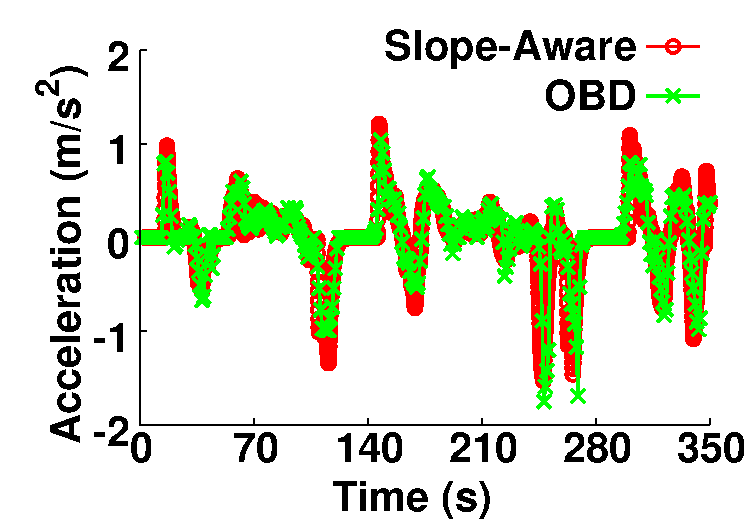
\includegraphics[width=2.2in,angle=0]{Figs/DriveSense/slopeaware/acccompare.pdf}
\hspace{-0.0cm}
\vspace{-0.2cm}
\caption{Slope-Aware coordinate alignment and linear acceleration estimation. 
The Figs/DriveSense are about acceleration over/under estimation caused by slopes (left), 
using gyroscope to estimate road slopes (middle), 
comparing estimated linear acceleration with groundtruth acceleration (right).}
\vspace{-0.2cm}
\label{linear_acceleration}
\end{center}
\end{figure*}


After coordinate alignment is complete, 
we can track the acceleration of a car by using the accelerometer's y-axis. 
We illustrate the acceleration values from aligned accelerometer 
in an example trip illustrated in Fig. \ref{linear_acceleration}. 
As the figure shows, comparing with the accelerations by OBD,   
the accelerations by the accelerometer of the first $90s$ 
are underestimated and the following $60s$ are overestimated.
This is because the car is moving mainly downslope and then mainly upslope. 
The deviated estimations may cause false positives/negatives on 
capturing driving behaviors such as brakes and accelerations.

We apply the same rotation matrix to the gyroscope data and 
illustrate the gyroscope x-axis data in Fig. \ref{linear_acceleration}.
After removing the constant drifts, 
it shows clear trends that the car is moving downslope and then
upslope.
Given the similar trends illustrated in two plots, 
we can estimate the slope gradient and deduct the gravitational force
components. 
We use similar calibration techniques proposed in \cite{zhou2014use}. 
We identify the road segments and stop points where accelerometer
can provide more accurate slope gradients to calibrate gyroscope.  



 

\subsection{Detecting Relative Orientation Change}


\begin{figure}[!htbp]
\begin{center}
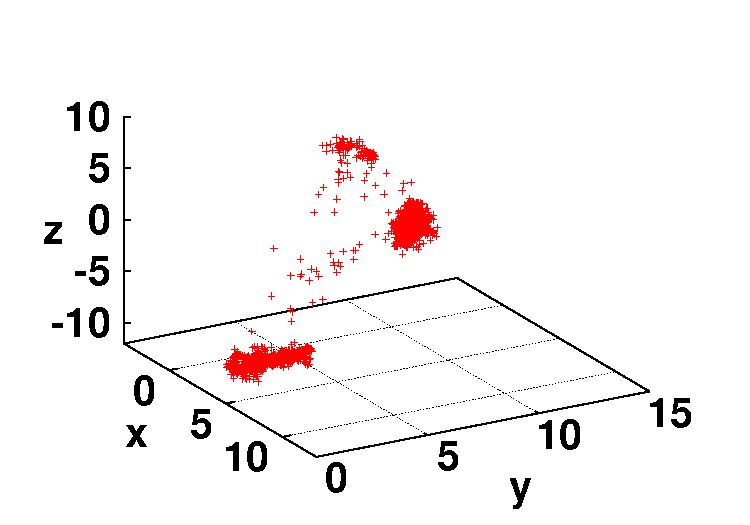
\includegraphics[width=1.7in,angle=0]{Figs/DriveSense/example_cluster.pdf}
\hspace{-0.8cm}
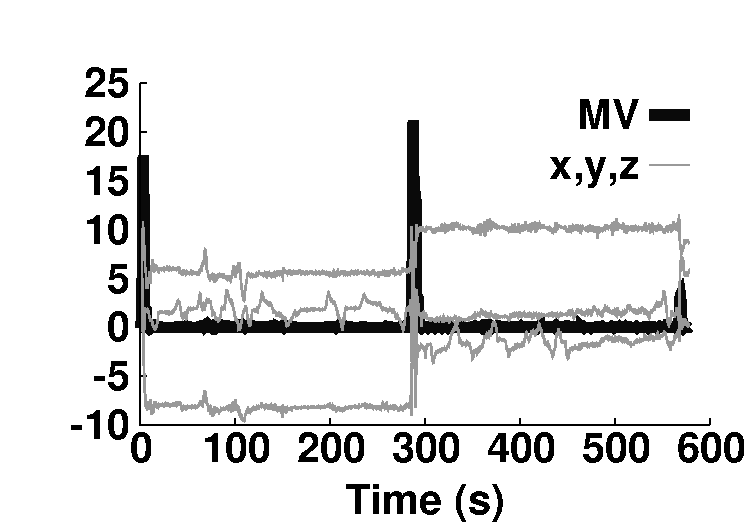
\includegraphics[width=1.7in,angle=0]{Figs/DriveSense/example_change.pdf}
\vspace{0.0cm}
\caption{The accelerometer data in one trip where the smartphone is picked up
from a pocket and put on the car mount holder. 
The upper cluster is formed when the user start the app at the beginning
and put the phone into the pocket, which is also detected by MV method. }
\vspace{-0.2cm}
\label{example_change}
\end{center}
\end{figure}


Using inertial sensors to estimate vehicle motions
is also vulnerable to smartphone relative orientation changes. 
Relative orientation refers to the relative orientation 
between the smartphone and the car.  
When the smartphone is fixed in the car and 
the car is moving upslope or making turns, the
relative orientation of the smartphone does not change 
as there is no relative movement between the smartphone
and the car.  
The relative orientation is usually changed by the smartphone
user, e.g., moving the smartphone from pocket to the car mount
for navigation.



The gyroscope is able to track absolute orientation changes
of the smartphone \cite{zhou2014use}. 
Tracking relative orientation change is a different. 
Since the smartphone is moving at the same pace 
with the car (suppose the smartphone is mounted), 
the gyroscope will sense the steering motions of the 
car, i.e., making turns, driving upslopes etc. 
It is challenging to separate the movement of the car
and the movement of the smartphone itself. 


We find accelerometer can be used to reliably detect orientation changes. 
While the movement of the car will introduce noises accelerometer
readings, but the noises are relatively small ($1-2m/s^2$ in most of the cases) 
in comparison to the gravitational force sensed by accelerometer. 
Once there is an orientation change, the gravity components
sensed by accelerometer are changed dramatically.
During one test trip, we move the smartphone
from pocket to car mount holder. 
The accelerometer sensor readings are illustrated in Fig. \ref{example_change}. 
All the accelerometer sensor readings can be naturally
classified into three clusters. 
The upper small one is formed when the user hold
the smartphone and manually start the app. 
The rest two are formed when the smartphone is in 
the pocket and on the car mount holder, respectively. 
Intuitively, incremental clustering methods are reasonable 
choices to identify orientation change, 
i.e., there is new cluster formed. 


\textbf{Incremental Clustering}. Traditional incremental clustering methods can be used in 
orientation change detection, e.g., 
orientation change happens when there is another cluster
emerges. 
The existing clustering methods are reliable enough
and tested by many applications 
\cite{nguyen2015survey, ordonez2003clustering, rodrigues2008hierarchical, song2005highly}. 
We test several common incremental clustering methods 
such as Sequential K-means (S-KM), Hierarchical Clustering (HCA) 
and Gaussian Mixture Models (GMM). 
The drawback of such approaches is the delay for detecting
another cluster, i.e., it requires enough data samples
to form a new cluster. 
In some real time applications such as brake warnings, 
false warning may happen if orientation change
is not detected in the first place. 
Due to the space limit, We refer interested 
readers to \cite{nguyen2015survey} for 
detailed descriptions of different methods.


\textbf{Moving Variance (MV)}. To timely detect orientation change before
another cluster is formed, 
we look at the change of a moving window.
The moving window contains $m$ data samples, 
and we use the variance of the moving window to detect
orientation changes. 
The intuition behind is that the changes of sensed gravity components 
is much more significant than those of caused by vehicle's movements. 
The variance can be calculated as $Var(x) = E[(X - \mu)^2]$, 
where $X$ is the euclidean distance to the ``moving cluster''
center and $\mu$ is the average distance. 
There are cases that the movement is too small to be detected
by MV. 
For example, a small horizontal rotation of the smartphone will not 
change the variance. 
We use the stability model to estimate such small changes. 
We will show in the later section that such looseness
make the acceleration estimation inaccurate. 
 
 
\subsection{Estimating Mounting Stability}



\begin{figure}[!htbp]
\begin{center}
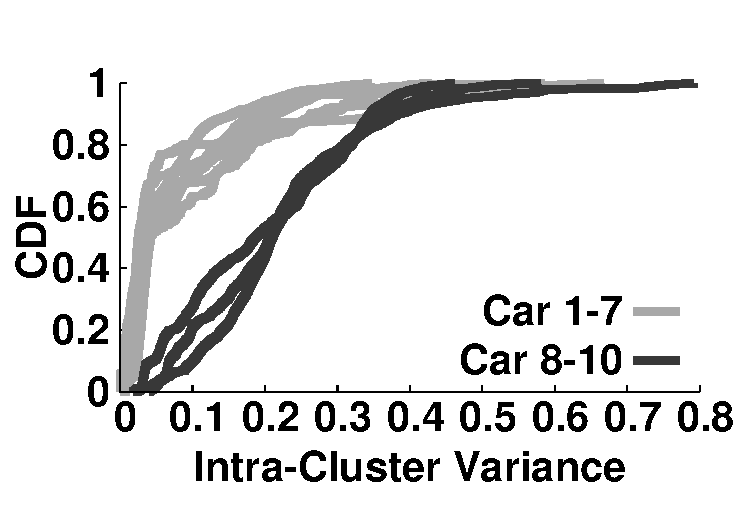
\includegraphics[width=1.7in,angle=0]{Figs/DriveSense/variance_cars.pdf}
\hspace{-0.5cm}
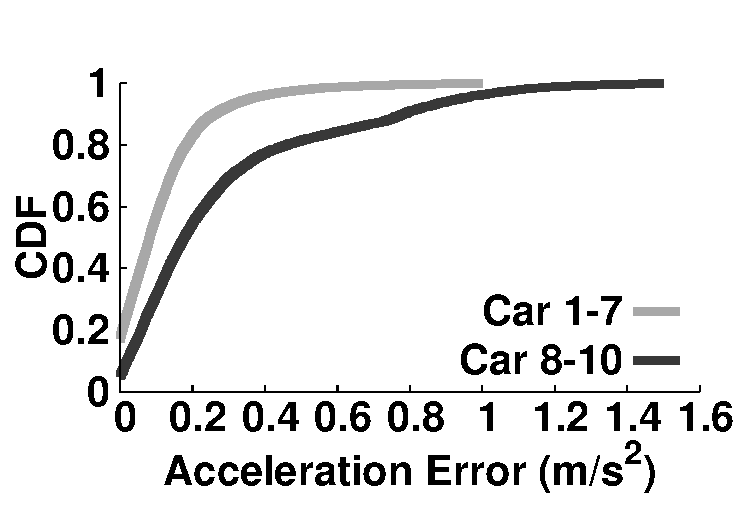
\includegraphics[width=1.7in,angle=0]{Figs/DriveSense/sensor_error_cars.pdf}
\vspace{-0.2cm}
\caption{The intra-cluster variance distribution of the tight group (car 1-7)
	and the loose group (car 8-10), and 
the estimated acceleration accuracy of the tight group is higher than those
	of the loose group.}
\vspace{-0.2cm}
\label{mounting}
\end{center}
\end{figure}


Another factor affects the accuracy of vehicle motion sensing
is the mounting stability of the smartphone. 
The stability of the smartphone depends on how the 
smartphone is fixed/placed/held in the car. 
A good case scenario is the user placing the smartphone
on a stable car mount holder. 
A bad case scenario is the user or passenger playing
motion games such as car racing which requires rotating
the smartphone. 
The derived sensor readings of the car are over noisy
due to shaking and/or rotating of the smartphone. 


We model one fixed relative orientation as a cluster of 
sensor readings. 
We use \emph{intra-cluster variance (ICV)} to estimate 
the stability of the smartphone.  
A stable mounting of the smartphone is expected to produce a smaller
variance than unstable holding by hands.  
Since ICV is correlated with the cluster
size, we use the ICV of the subclusters to represent
the ICV of the whole cluster. 
We define one subcluster is any continous $n$ 
points of the whole cluster.  
We use ICV to evaluate the mounting
stability of the tablets from dataset $\#1$. 
We firstly remove all the trips that there is orientation 
change detected. 
As shown in Fig. \ref{mounting}, 
all the data from the 10 cars are naturally divided into two groups, 
where the first group (car 1-7) has a median variance less than 0.05
and the second group (car 8-10) has a median variance around 0.2.
We name the first group as \emph{tight group} and 
the second one as \emph{loose group}. 
Since the tablets are not aligned with the cars, 
we conduct coordinate alignment and linear acceleration
estimation by using the methods in Section \ref{slopeaware}. 
We compare the acceleration estimated by aligned accelerometer
and the groundtruth acceleration calculated by OBD speed. 
As indicated in Fig. \ref{mounting}, 
the estimated accuracy of the tight group is generally higher
than the loose group. 


  





\section{The Promise of GPS in Driving Analytics}
\label{gps}


GPS is the most ubiquitous localization system and generally
provides absolute coordinates. 
The usability of GPS in driving analytics has not been 
well discussed by the communities due to its high energy cost 
and coarse-grained measurements. 
Our measurements indicate GPS is a good 
candidate especially when IMU sensor
is not available to use or less accurate. 
We find that GPS has high accuracy in 
estimating speed and accelerations, 
especially in high speed scenarios (e.g., >10m/s).  
Given the simplicity of acceleration estimation
and high accuracy of GPS, 
we believe inertial sensors can be 
augmented by GPS in vehicle speed and acceleration
estimation applications. 




\nop{
Recently, Google announced that the raw data (e.g., pseudoranges, Dopplers and carrier phase) 
of GPS receiver is accessible for Android 7.0 \cite{android_gnss, google_gnss_tools}. 
}

\subsection{How GPS Works}

GPS provides a simple way to track vehicle motions
due to its orientation independent nature.
However, it has been blamed for its low
accuracy \cite{hedgecock2013high, gowda2016tracking}.
A GPS receiver can compute the instant absolute location
by receiving ephemeris data transmitted from satellite systems. 
The GPS satellites transmit signal with the starting 
time of the transmission (obtained from the satellites' atomic clock). 
Meanwhile, the ground receiver records the time of reception with 
smartphone local clock. 
The flight-time is the gap between these timestamps. 
The major error is caused by the smartphone GPS receiver
clock biases \cite{hedgecock2013high, gowda2016tracking}. 
Considering we are interested in the relative position of 
two continuous measurements from the same GPS receiver, 
the clock biases of the measurements are neutralized. 
In this work, we use smartphone built-in GPS as 
an augmenting method for driving analytics. 
We leave the performance gain by utilizing GPS raw data for the future work.


\subsection{Speed Estimation}

\begin{figure}[!htbp]
\begin{center}
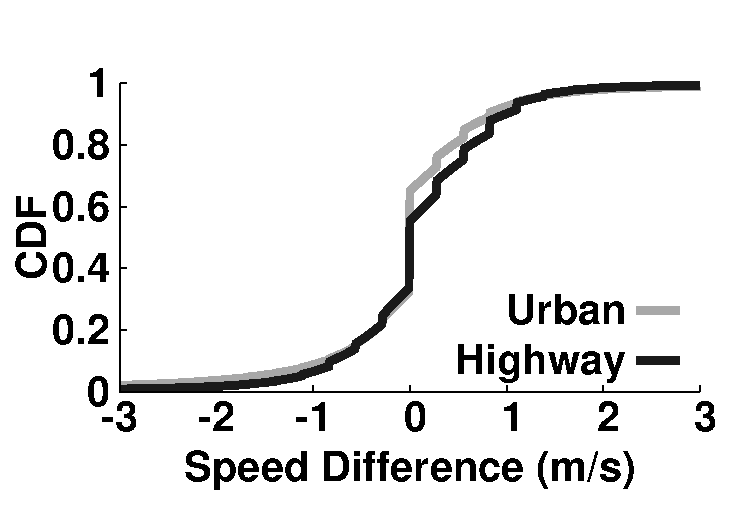
\includegraphics[width=2.6in,angle=0]{Figs/DriveSense/gpsobd_speed_diff.pdf}
\vspace{-0.2cm}
\caption{The speed estimation error of GPS.}
\vspace{-0.2cm}
\label{speeddiff}
\end{center}
\end{figure}

Speed calculation is very important for many vehicular applications \cite{hansenspeed, chandrasekaran2010vehicular}.  
GPS can provide speed information by simply calculating
the distance and time difference between two adjacent points. 
We use dataset $\#1$ (more details in section \ref{evaluation}) to evaluate the speed estimation of GPS. 
We tag the dataset with highway trips and urban trips,
based on speed distributions. 
Trips with a speed over $50mph$ in any segment is classified into highway trips. 
The CDF of speed estimation errors are plotted in Fig. \ref{speeddiff}. 
More than $90\%$ of the points are able to accurately calculate the speed 
with the error less than $1m/s$. 


\subsection{Acceleration Estimation}



\begin{figure}[!tb]
\begin{center}
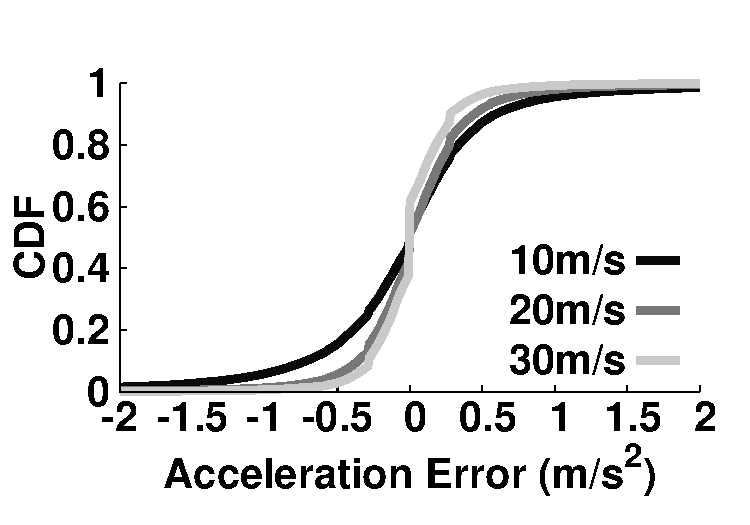
\includegraphics[width=3.0in,angle=0]{Figs/DriveSense/gpsobd_acce_speed.pdf}
\vspace{-0.2cm}
\caption{Acceleration estimation errors of GPS in urban and highway environments. 
	The estimation is more accurate in higher speed ($>10m/s$) than lower speed ($<10m/s$).}
\vspace{-0.2cm}
\label{accediff}
\end{center}
\end{figure}


The acceleration is comparatively evaluated by GPS points and OBD speed data.  
The CDF of estimation error is shown in Fig. \ref{accediff}. 
Each curve stands for the acceleration estimation error no more than that speed, i.e., 
$10m/s$ refers to any speeds not higher than $10m/s$ and $20m/s$ refers to any speeds between $10m/s$ and $20m/s$. 
The estimation errors of GPS in low speed are caused by GPS location estimation errors, which could be caused by either the weak GPS satellite signal or strong thermo-noise floor. 
Additionally, the errors could also be caused by the building and vehicle blockage.  
The acceleration estimation when the vehicular speed is higher than $20m/s$ 
is highly accurate. 
This result indicates that GPS is more accurate in high speed scenarios.




\subsection{GPS Availability}



\begin{figure}[!tb]
\begin{center}
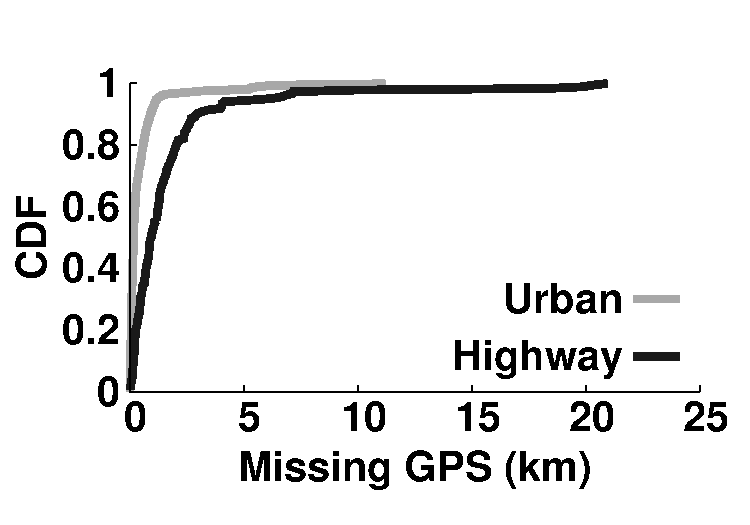
\includegraphics[width=1.7in,angle=0]{Figs/DriveSense/missing_gps.pdf}
\hspace{-0.5cm}
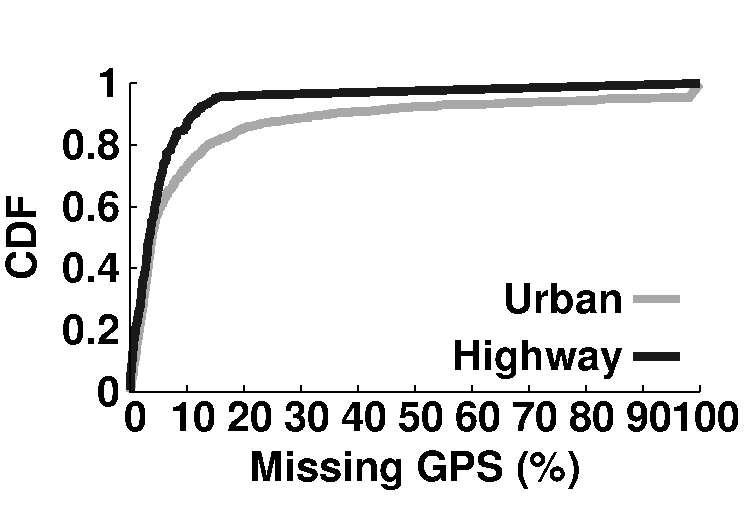
\includegraphics[width=1.7in,angle=0]{Figs/DriveSense/missing_percent.pdf}
\vspace{-0.2cm}
\caption{GPS availability in urban and highway environments. }
\vspace{-0.2cm}
\label{missinggps}
\end{center}
\end{figure}


GPS signal is not always available, especially in indoor
environments.
If the smartphone is inside the car, there are chances
that the smartphone GPS receiver is not able 
to detect satellite signals.  
Also, if the car is passing through underground tunnel or high buildings, 
GPS signal might be too weak to be received. 
We compare GPS and OBD data point by point, 
and record the accumulated distance of trip fragment without GPS points. 
The missing GPS of each trip is illustrated in Fig. \ref{missinggps}. 
There are a couple of trips that are entirely missing, 
while we are not sure if it is caused by software bugs or blocked signals. 
The GPS is available most of the time, while there are cases
that the GPS is missing at the start and/or end of the trip. 




 


%%%%%%%%%%%%%%%%%%%%%%%%%%%%%%%

\nop{
\subsection{Steering Angle Estimation}

\begin{figure}[!htbp]
\begin{center}
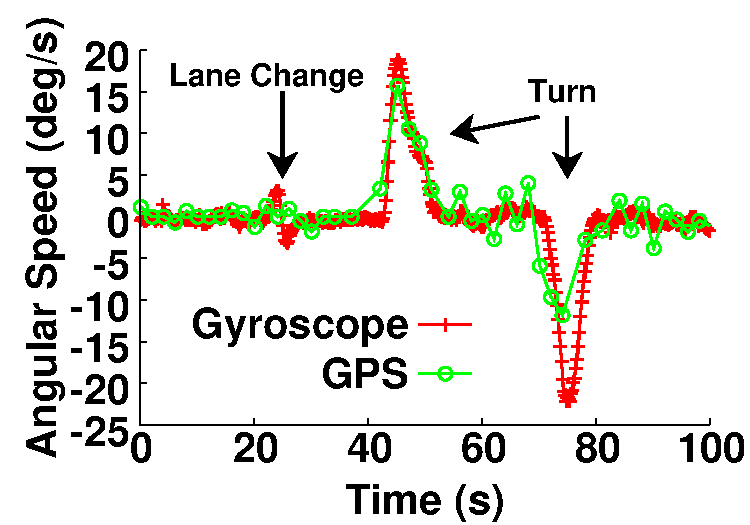
\includegraphics[width=2.6in,angle=0]{Figs/DriveSense/angular_illustration.pdf}
\vspace{-0.2cm}
\caption{An illustration of steering angular velocity estimation of GPS.}
\vspace{-0.2cm}
\label{steeringillustration}
\end{center}
\end{figure}

\begin{figure}[!htbp]
\begin{center}
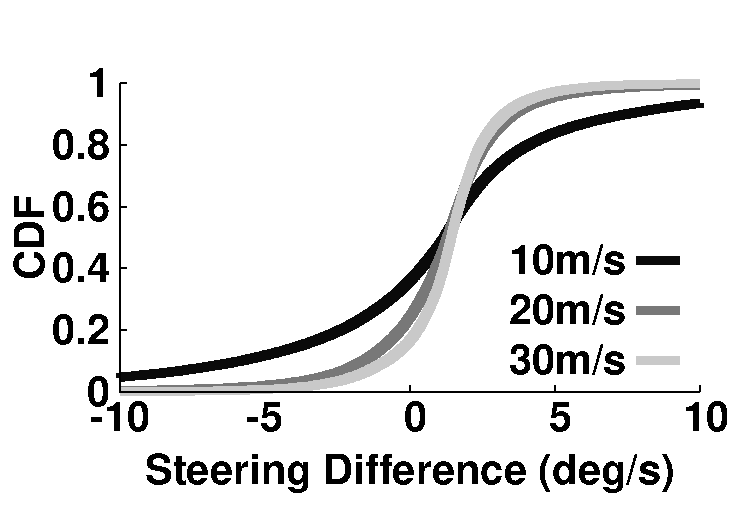
\includegraphics[width=2.6in,angle=0]{Figs/DriveSense/gps_steering.pdf}
\vspace{-0.2cm}
\caption{The GPS steering angular velocity estimation difference comparing with gyroscope.}
\vspace{-0.2cm}
\label{steeringdiff}
\end{center}
\end{figure}

Another important aspect of vehicle motion is steering motion. 
GPS can be used to estimate the changes of steering angle
by using a two pass processing. 
The first pass is used to calculate the moving direction
based on two GPS point. 
The second pass is used to calculate the angular attitude
rate based on direction differences. 
There are more noises on GPS readings
in low speed, i.e., the GPS indicates the vehicle is 
moving while the car is actually not, or the vehicle is stable but the GPS indicate the movement. 
Using adjacent points to calculate the direction introduces
lots of noises. 
We use the next GPS point at least $l-meter$ 
away as the next hop to calculate the direction. 
We compare the angular attitude rate estimated by GPS with
the ones estimated by 
gyroscope.
A trip fragment is illustrated in Fig.\ref{steeringillustration}
and the statistics are plotted in Fig. \ref{steeringdiff}.
Three observations can be concluded from this two Figs/DriveSense. 
First, the steering angular velocity estimated by GPS
is very coarse-grain, and cannot be used
for small direction movement such as lane changes. 
To detect the lane change, a precision of $0.5deg/s$ 
is required, while more than $80\%$ of the 
estimation error (by GPS) is higher than $1deg/s$.
Second, GPS can be used to identify large direction
changes such as turns, e.g., GPS can detect $83.54\%$
of the turns detected by gyroscope. 
GPS is very noisy when steering around parking lot
and cannot used for motion detection. 
Third, similar to acceleration estimation, 
the estimation accuracy of angular velocity is higher 
in high speed scenarios. 
}





\section{Design and Implementation}
\label{design_implement}




\subsection{Design of XSense}


\subsubsection{Workflow}

\begin{figure}[!htbp]
\begin{center}
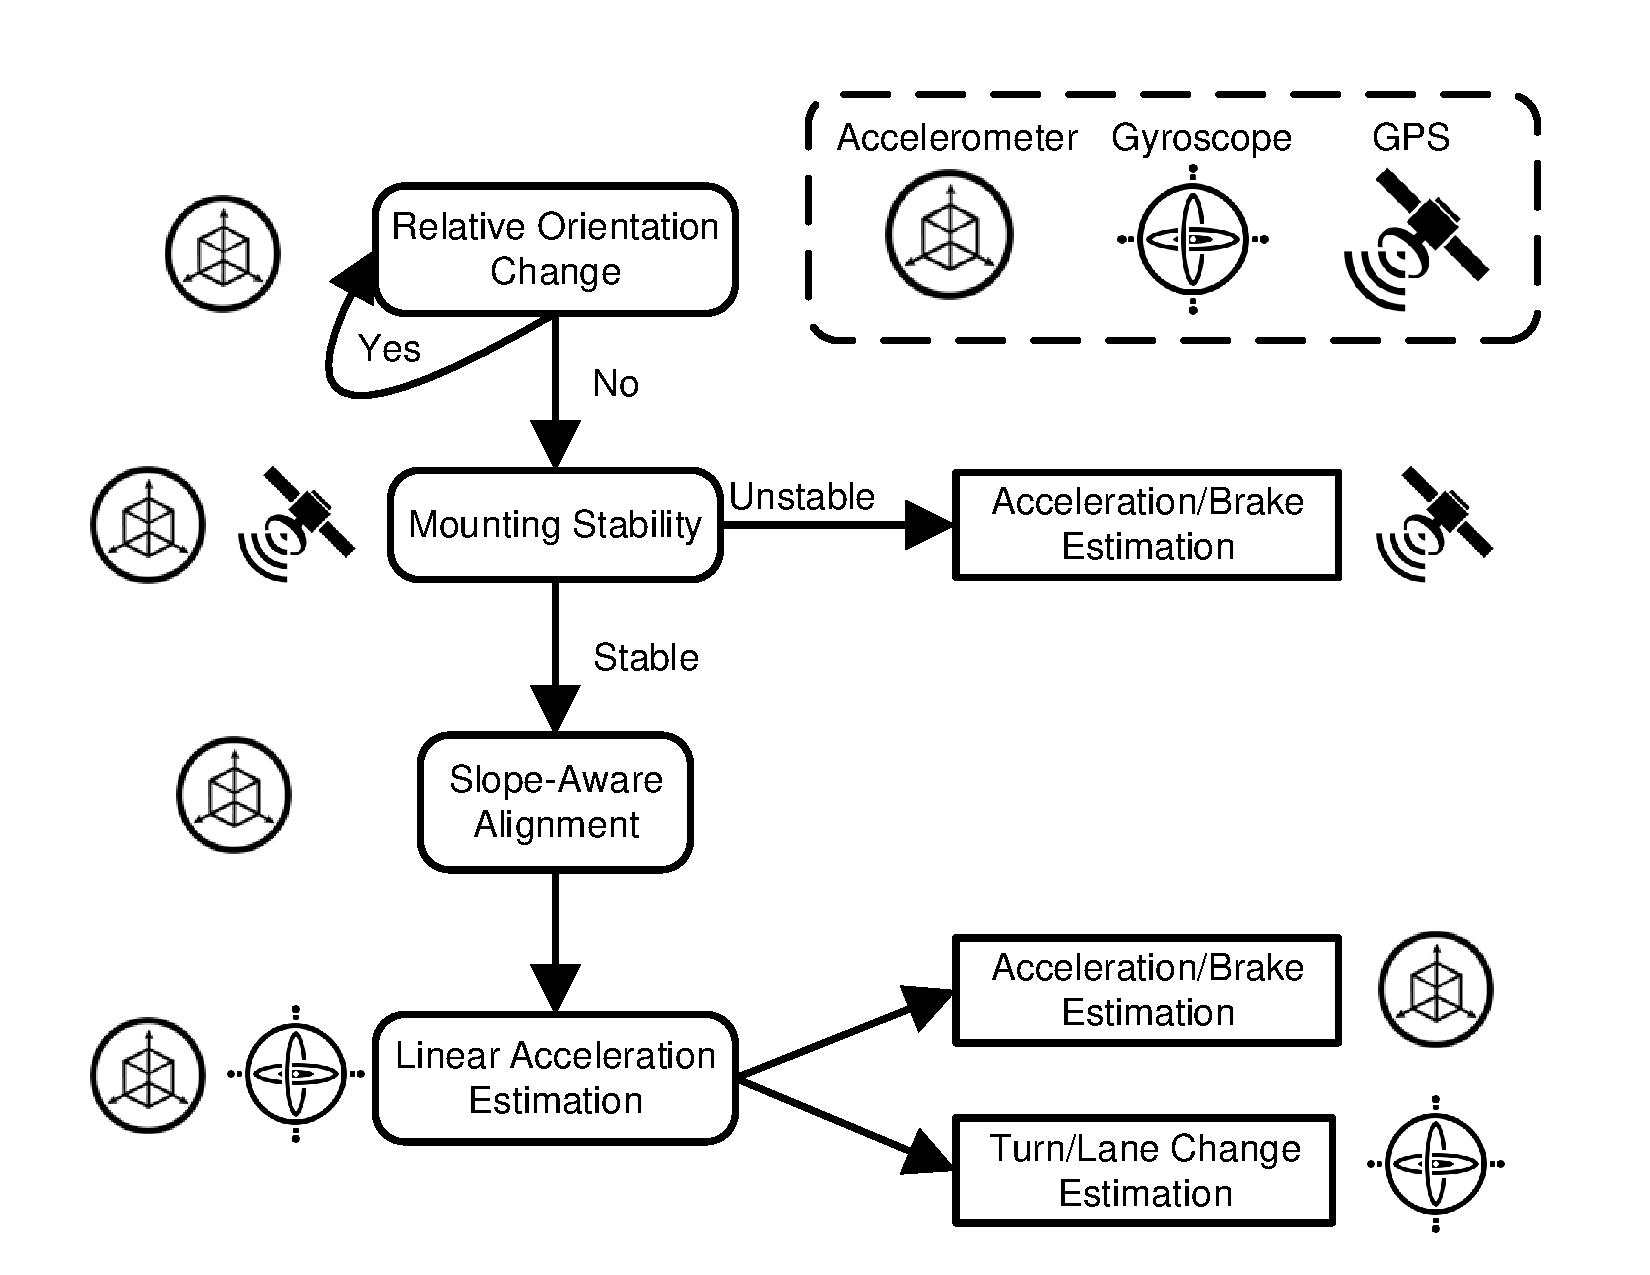
\includegraphics[width=3.6in, angle=0]{Figs/DriveSense/system_flowchart.pdf}
\vspace{-0.2cm}
\caption{Workflow of XSense.}
\vspace{-0.6cm}
\label{workflow}
\end{center}
\end{figure}


The workflow of XSense is illustrated in Fig. \ref{workflow}. 
XSense uses several modules to evaluate sensor
performance and estimate vehicle motion paramters. 
The inputs of XSense are accelerometer, gyroscope
and GPS.  
In each module, it uses different sensors as input.  
The corresponding sensor icon is placed along with the 
module if it requires that sensor as input.  
Our method uses the accelerometer extensively
as it provides a baseline by measuring the absolute acceleration while
the gyroscope measures only relative angular speed. 
The first module is to detect relative orientation changes.  
If an orientation change is detected, 
XSense will restart the rotation matrix
training process until the 
relative orientation of the phone is fixed.  
The second module is called stability monitoring
module, which is used to monitor the mounting
stability of the smartphone. 
The stability of the smartphone is quantified
by a threshold, which depends on the 
accuracy of GPS and that of the accelerometer. 
If the accuracy of the accelerometer is higher
than that of GPS, we think the smartphone
is mounted stably. 
In other case, we use GPS to estimate acceleration.
The third one is slope-aware coordinate
alignment module, 
which aligns the coordinates from the smartphone
to those of the car and estimates
the gradients of the training road segment. 
Both horizontal and vertical alignment are conducted
in this module. 
The last one is the linear acceleration estimation
module, which is used to estimate the slope 
gradients along the way.
XSense may selective use GPS or accelerometer
to estimate accelerations based on
the accuracy of each method. 
The accuracy comparison between GPS and accelerometer
is illustrated in section \ref{evaluation}. 



\subsubsection{Fusion with GPS}


GPS can be used to detect accelerations and brakes
when the IMU sensors are not available or not
ready to be used. 
IMU sensor is not available when the user 
frequently changes the relative orientation of the smartphone
or does not mount the smartphone stably. 
For example, if the user is holding the smartphone
to play game or send text message, 
the IMU sensor readings are too noisy 
to use. 
Even the user mounts the smartphone in a 
fixed place, it takes tens of seconds to minutes 
to collect enough data for training the rotation matrix. 
During the training process, the 
IMU sensors are not ready to be used.  
\footnote{The accelerometer takes much longer than gyroscope
as the gyroscope does not sense gravity.}


The GPS can also be used to eliminate the movement of the vehicle
when modeling mounting stability. 
We subtract the acceleration measured by the GPS from
the acceleration measured by the accelerometer. 
To do this, we project the 3D acceleration measured
by accelerometer into 2D space. 
Ideally, one dimension of senses gravity and the other
senses the horizontal movement of the car. 
For simplicity, we projects the 2D horizontal 
acceleration sensed by the accelerometer
into a single dimension and use it to subtract the acceleration
measured by GPS. 
We use this method only when the speed measured by GPS
is higher than a threshold. 


\subsection{Implementation}


We implement XSense as a software module in Java and 
import it to an Android application we wrote.
To make our test easier, we develop an offline 
trace replay engine.
The replay engine sorts the sensor data
based on timestamps, and feeds them into an event listener function in chronological order. 
We use an abstraction called \emph{Trace} to represent the sensor data, 
GPS data and OBD parameters.
It is similar to SensorEvent used by Android API \cite{sensor}
and provides additional flexibility to store OBD and GPS data. 
The event listener function process each \emph{Trace} 
according to corresponding sensor type.  
The trace replay engine makes it easier to import
XSense to the Android application. 
The Android application is aiming to monitor and record
daily driving trips. 
The app is implemented by less than 4,000 lines of Java code, 
but supports a variety of functionalities such as
trip recording, real time display, trip management,
trip display on Google map, user management and access control, 
online/offline uploading, data synchronization with remote server etc. 
XSense serves as a module that provide an more accurate
estimation on vehicle motions, e.g., hard brakes. 
For this submission, we highlight XSense module 
and remove some functionalities such as
trip upload, user management etc.
The QR code for a link to download the xsense.apk package is provided in Fig. \ref{xsense_app}. 

\begin{figure}[!tb]
\begin{center}
%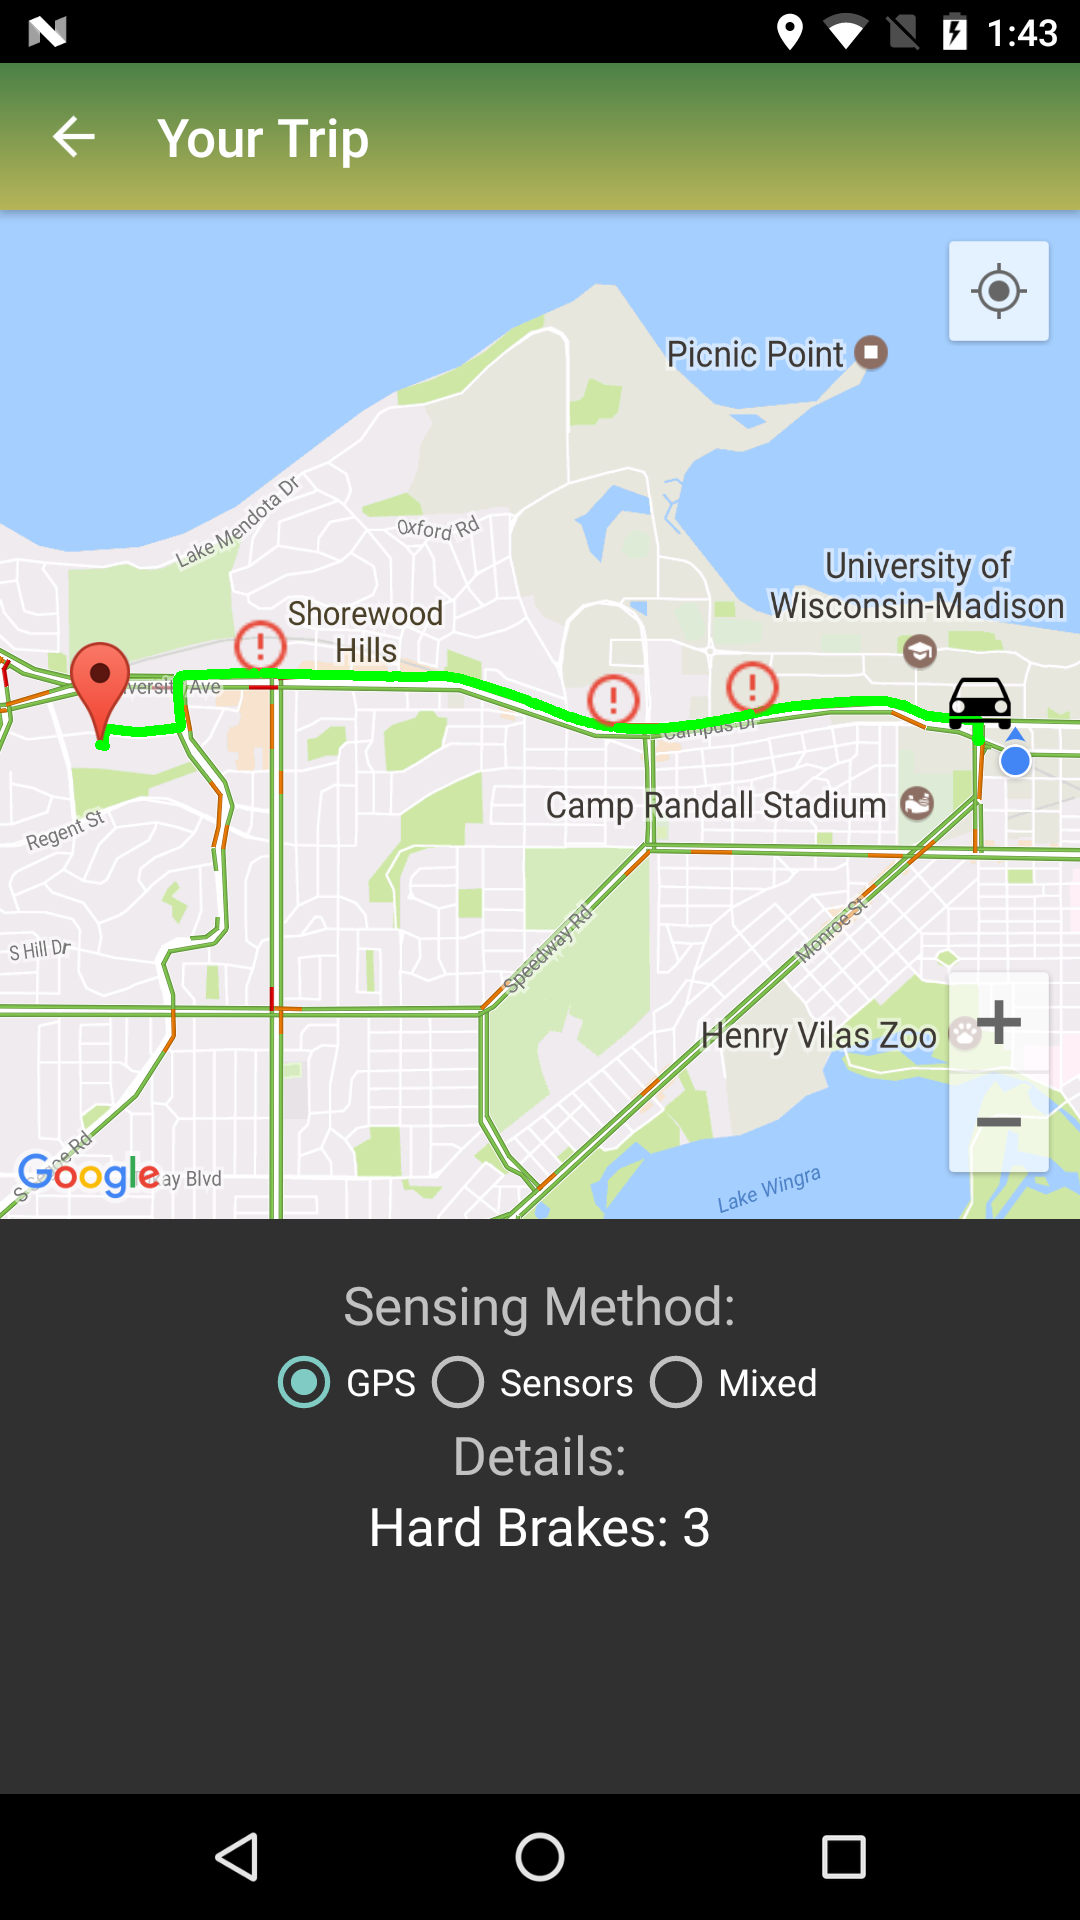
\includegraphics[width=1.7in,angle=0]{Figs/DriveSense/screenshot_gps.png}
%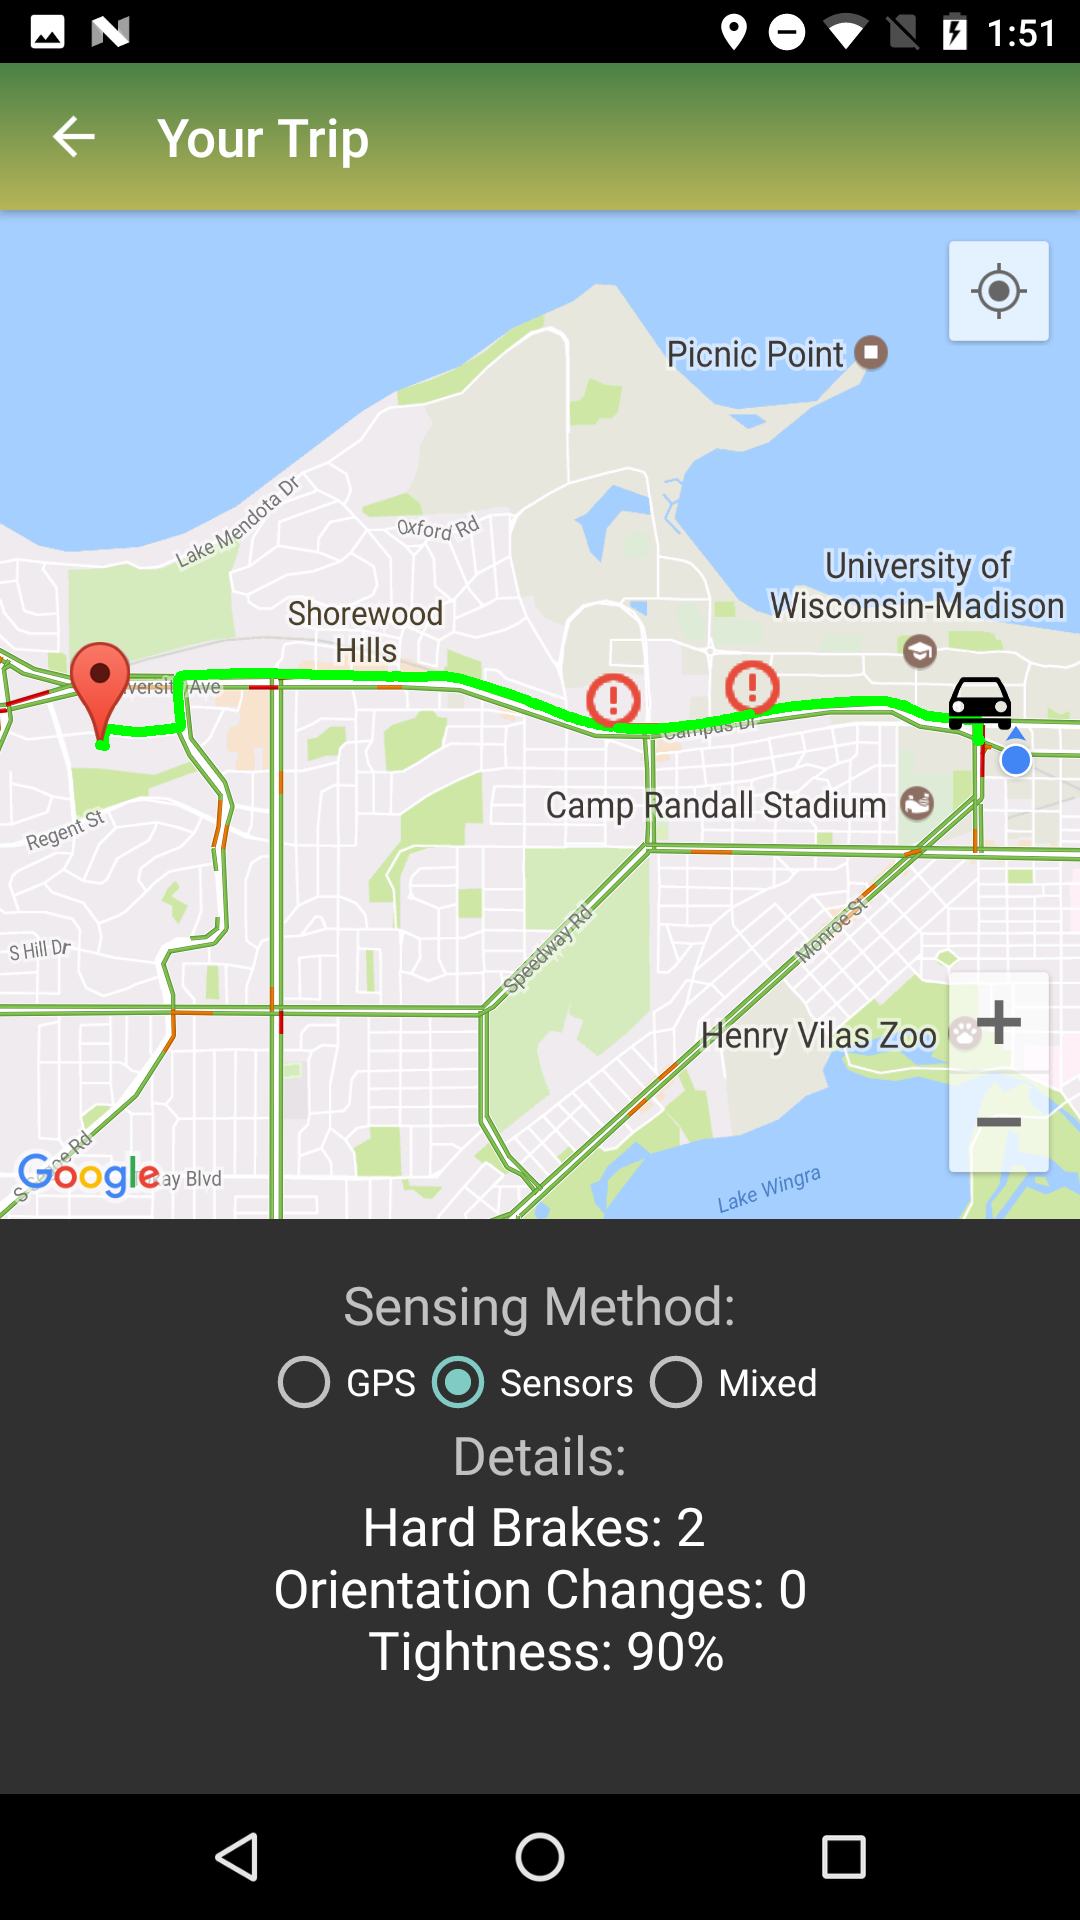
\includegraphics[width=1.7in,angle=0]{Figs/DriveSense/screenshot_sensors.png}
%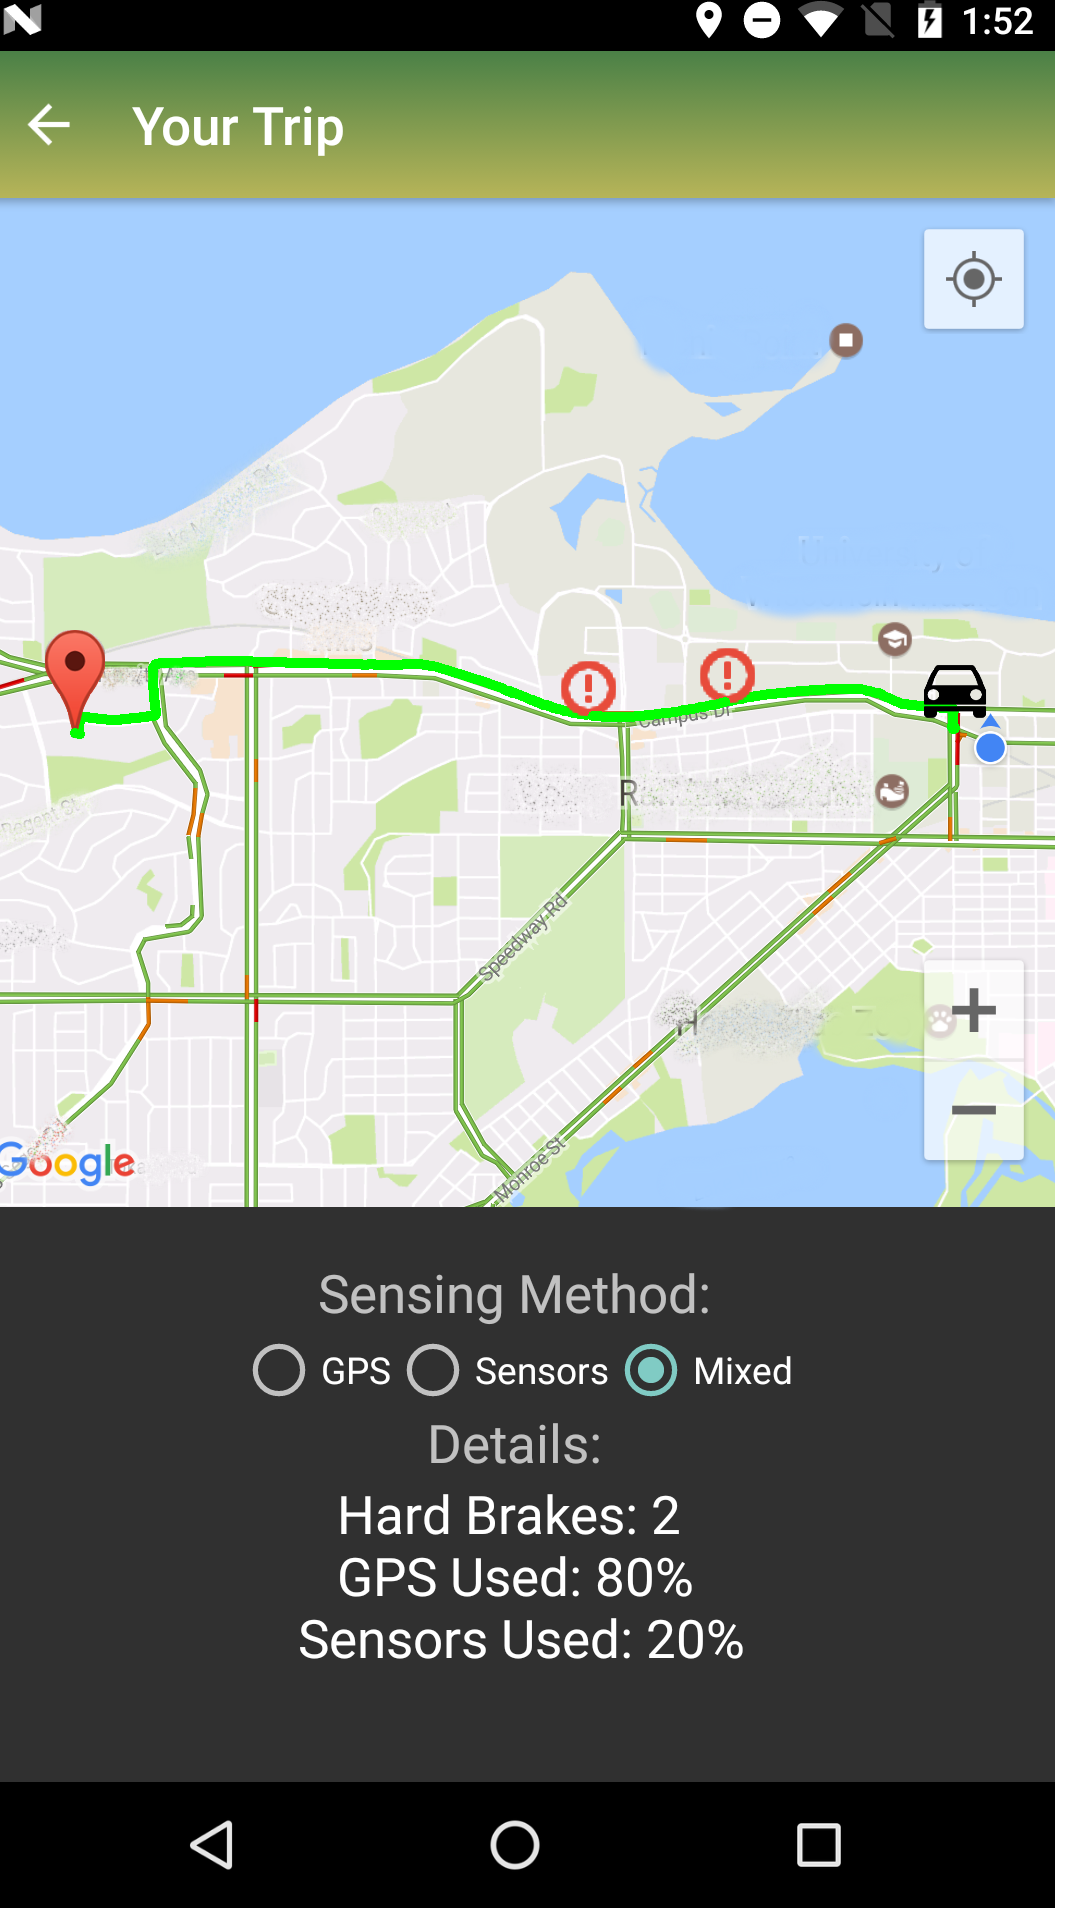
\includegraphics[width=1.8in, angle=0]{Figs/DriveSense/screenshot_mixed_hidden.png}
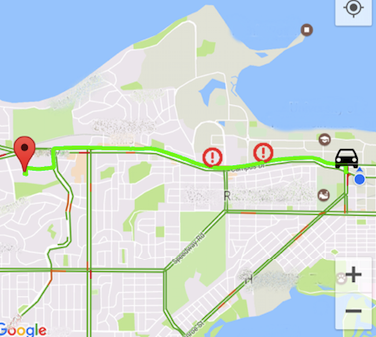
\includegraphics[width=1.8in, angle=0]{Figs/DriveSense/cut_app.png}
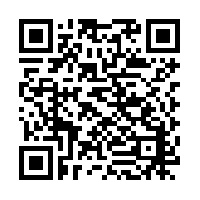
\includegraphics[width=1.4in, angle=0]{Figs/DriveSense/qrcode_xsense.png}
	\vspace{0.0cm}
\caption{The screenshot of XSense that user can view the hard brakes
	detected by GPS, sensors or mixed. The QR code can be scanned 
	to download the .apk Android installation file.}
\vspace{-0.2cm}
\label{xsense_app}
\end{center}
\end{figure}





\section{Experimental Results}
\label{evaluation}


\subsection{Dataset}

We use three datasets in our study. 
All of the datasets are collected by a gradually 
improved Android app.  
There are totally more than 13,000 miles of driving data 
collected in both controlled and uncontrolled environments
over the past three years.  
We will make our dateset available to public after 
this work has been published.  


\textbf{Dataset $\#1$}. 
We deploy Xoom tablets installed with our app on 10 different cars. 
The tablets collect the vehicular speed data from the On-board diagnostics (OBD)
port and various sensor data (including GPS and inertial sensors).  
Each tablet is placed in the back pocket of the passenger seat. 
The invovled cars are from different models and the stability
of the tablet placement is different, 
which provides the opportunity to study the effects of 
mounting stability on motion estimation accuracy.   


\textbf{Dataset $\#2$}.
We also collect some data in more controlled environments, 
where we know what is happening and the groundtruth data are recorded. 
First, we collect the data when the smartphone is placed in various scenarios, 
i.e., holding by hand, fixed by car mount holder, placed in cup holder etc. 
These data are used to understand various orientations and 
the relation between mounting stability and motion estimation accuracy.  
Second, we collect some data when randomly changing the 
orientation of the smartphone, i.e., 
move the smartphone from pocket and fix it on car mount holder. 
These data are used to evaluate the accuracy of 
our orientation change detection module. 
Third, we collect some data from two devices, where one device
is manually aligned with the car (as best as we can), 
and the other is fixed in car mount holder or held in passenger's hand. 
These data are used in two cases. 
One trip is used to understand acceleration
overestimation problem caused by gravitational force. 
Another 10 trips are used to estimate the
vehicle steering motions, where the gyroscope readings 
of manually aligned device is used as groundtruth data. 
 

\textbf{Dataset $\#3$}. 
We release the beta version of the Android app 
to 9 volunteers. 
The trip recording module is written as an Android Service,
so it is running in the background while the user may use 
the smartphone for navigation, game or any other activities. 
These data are used to understand how different users
are placing their smartphones while driving or 
sitting in the car. 



\subsubsection{Road Slope Statistics}

\begin{figure}[!htbp]
\begin{center}
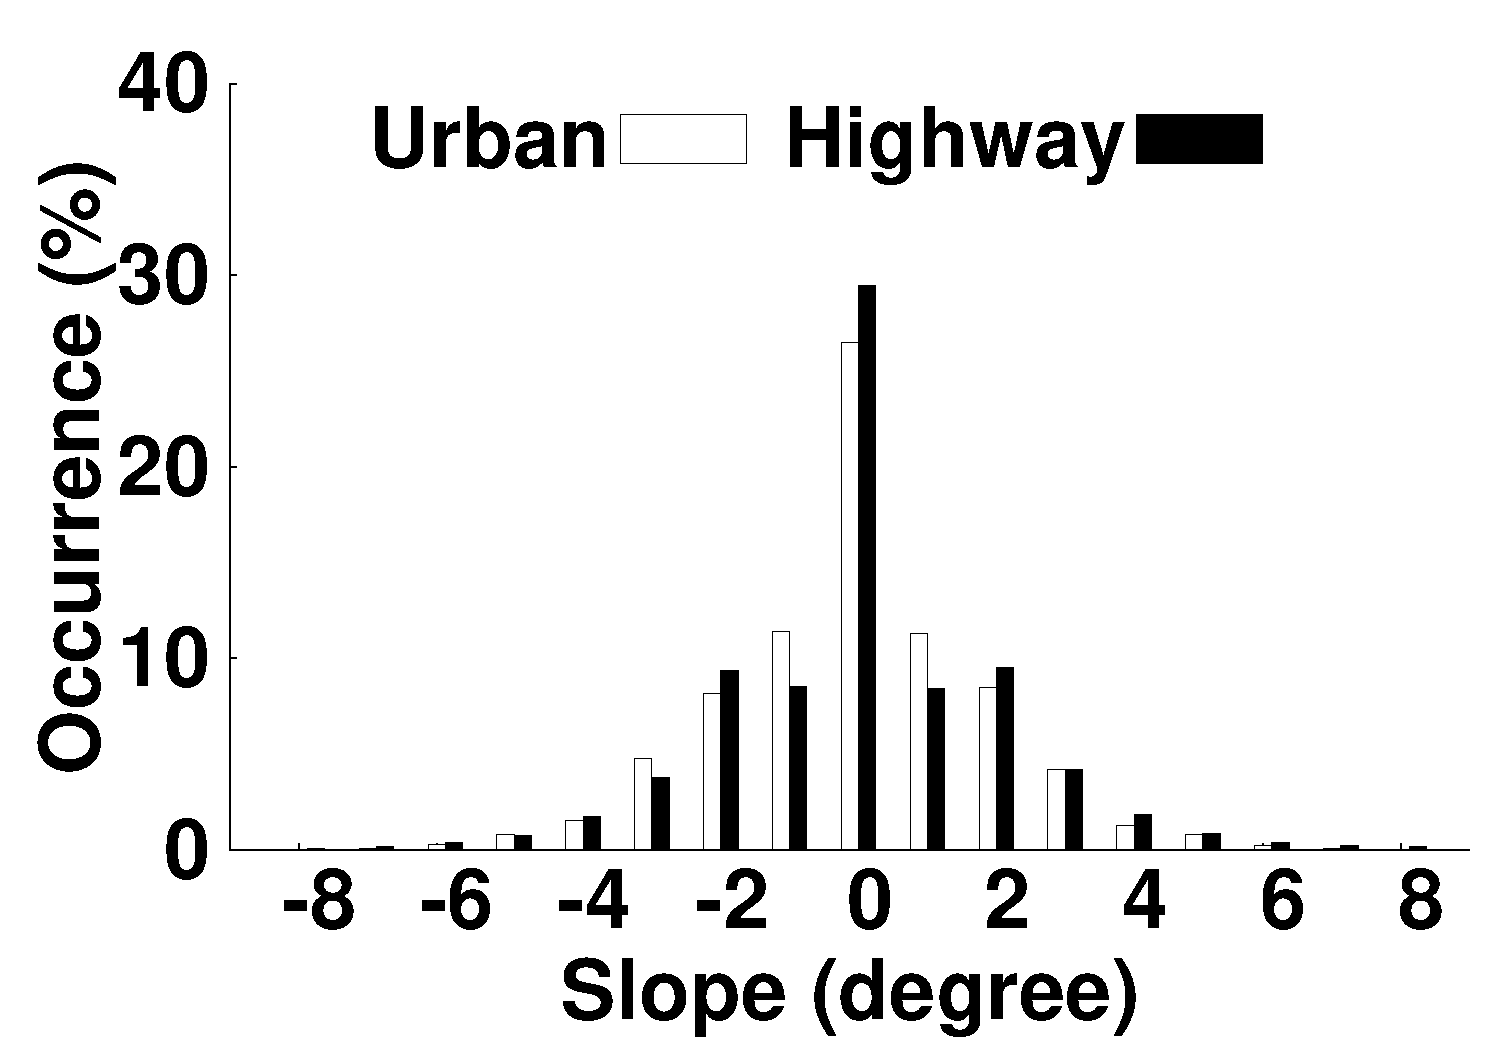
\includegraphics[width=2.5in, angle=0]{Figs/DriveSense/slopeaware/degrees.pdf}
%\hspace{-0.6cm}
%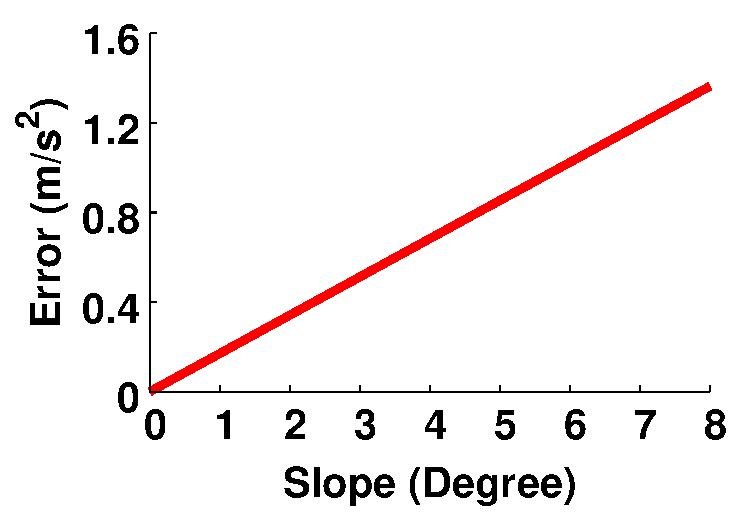
\includegraphics[width=2.5in, angle=0]{Figs/DriveSense/slopeaware/slope_error.pdf}
%\vspace{0.0cm}
%\caption{Histogram of slope gradients (left) and acceleration estimation errors 
%	under different slope gradients (right).}
\caption{Histogram of slope gradients. The acceleration estimation error is 
proportional to $gsin\theta$, where $\theta$ is the road slope angle.}
\label{slopegradients}
\vspace{-0.4cm}
\end{center}
\end{figure}


As we discussed above, the slopes introduce linear acceleration estimation errors.
An important question is how many road segments are sloping and
how many of them are actually level. 
Some cities, e.g., San Diego and Los Angeles, are full of hills, 
and most roads are sloping roads.
Surprisingly, in a plain area in US where we collect data, 
there are also full of slopes. 
To obtain the road gradient, we use the Google elevation dataset \cite{googleelevation}. 
For each GPS data point, we queried the elevation from the dataset. 
and calculated the gradient by the elevation difference
and distance.
We eliminated the close consecutive GPS data points that less than 5 meters in distance and removed the data points where the speed is less than $10mph$.
As we can see from the histogram in Fig. \ref{slopegradients}, 
more than half of the roads are not flat.
Those sloping roads, even as small as two degrees, may introduce accumulated
errors on coordinate alignment and further slope estimation, i.e., $0.34m/s^2$.
The aggregated error may cause significant linear acceleration estimation error
and introduce false positives/negatives on brake/acceleration monitoring. 




\subsection{Improved Overall Accuracy}

\subsubsection{Acceleration Estimation}


We use dataset $\#1$ to evaluate the accuracy of DriveSense and
other methods. 
The other three methods are using Accelerometer with Traditional Coordinate
Alignment (TCA)  \cite{hansenspeed, wang2013sensing, chen2015invisible}, 
Slope-Aware coordinate alignment with linear 
acceleration estimation, 
and GPS.
In this evaluation, we only use the tight group data where the 
tablet is stably fixed in the car.  
Therefore, the results generated by sensors are 
the best cases can be achieved for sensor-based motion estimations. 
We compare the acceleration difference between
each method and the groudtruth (calculated by OBD speed). 
The results are shown in Fig. \ref{xsense_accuracy}. 
The estimation made by well-tuned sensor coordinate alignment and 
linear acceleration estimation (Slope-Aware curve)
shows similar $80\%$ accuracy with GPS. 
The gap between Slope-Aware and Accelerometer are caused
by road slopes, 
where slope-unaware solution will over/under-estimate 
acceleration due to gravitational force. 
The accuracy gain of DriveSense is from the 
acceleration estimation compensation by sensors
when the GPS speed is low. 

 

\begin{figure}[t]
\begin{center}
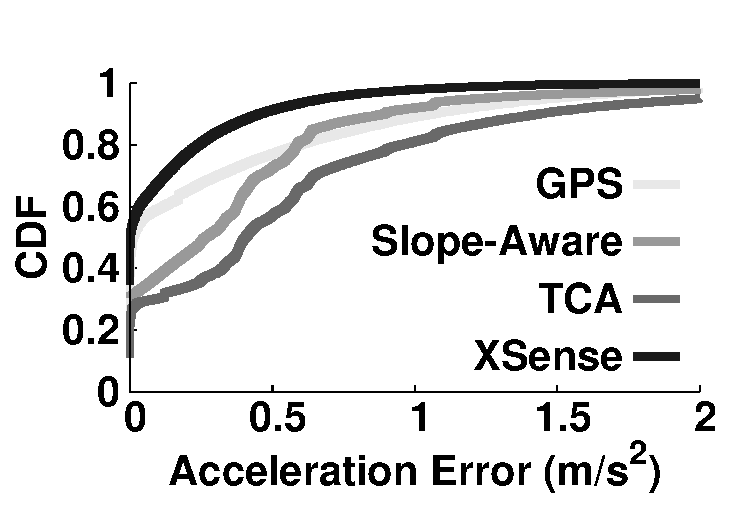
\includegraphics[width=3.0in,angle=0]{Figs/DriveSense/evaluation/xsense_accuracy.pdf}
\vspace{-0.2cm}
\caption{Comparing acceleration estimation accuracy among various methods.}
\vspace{-0.3cm}
\label{xsense_accuracy}
\end{center}
\end{figure}





\subsubsection{Steering Angular Velocity Estimation}


\begin{figure}[!htbp]
\begin{center}
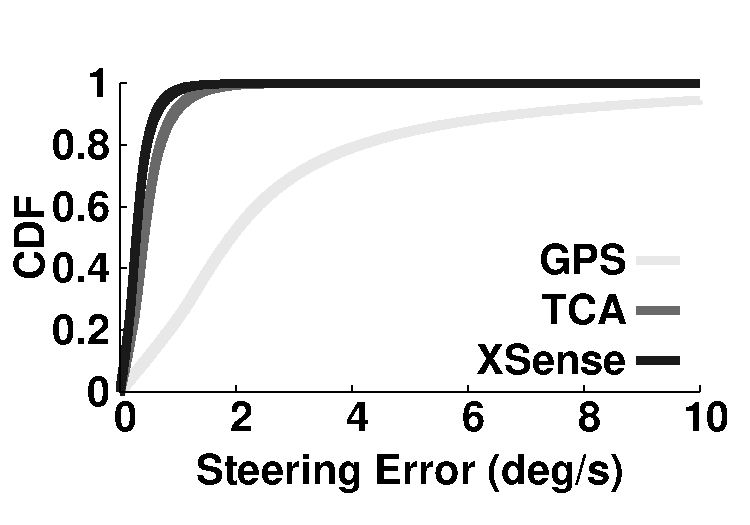
\includegraphics[width=3.0in,angle=0]{Figs/DriveSense/evaluation/evaluation_steering.pdf}
\vspace{-0.2cm}
\caption{Comparing steering angular velocity estimation accuracy among various methods. }
\vspace{-0.3cm}
\label{xsense_steering}
\end{center}
\end{figure}

We use dataset $\#2$ to evaluate steering angular velocity 
estimations. 
In this setting, one device is manually aligned with
the car and the gyroscope reading of which is used
as the groundtruth. 
Another device is fixed in car mount holder.    
As expected and can be seen in Fig. \ref{xsense_steering}, 
GPS can not estimate angular velocity accurate enough
for small horizontal movement such as lane change due to
its large estimation errors. 
DriveSense performs slightly better than gyroscope with 
Traditional Coordinate Alignment (TCA) due to 
the slope-aware solution presented in this work. 
The gain is obtained in the cases where the coordinate
alignment is conducted on slope, and there is vertical
misalignment caused by slope-unaware coordinate alignment. 




\subsection{Orientation Change Detection}

We evaluate the orientation change module
by using dataset $\#2$ in this section. 


\textbf{Detection Rate}.
The performance of inertial sensors in vehicle
motion sensing applications highly depends
on the fixed relative orientation between
the smartphone and the car. 
Therefore, detecting orientation change is 
very important in such applications. 
We evaluate the orientation change detection methods 
in two settings, tight setting and loose setting. 
In tight setting, the smartphone is mounted in 
various orientations on the car mount holder, 
or mounted by car cup holder. 
In loose setting, the smartphone is put in 
pocket, placed in passenger seat, or holding by 
passenger's hand. 
For each orientation, we record 
the groundtruth by a customized app. 
We use more than 10 trips and record
98 orientation changes in tight setting 
and 82 orientation changes in loose setting. 
The detection rate is presented in Table \ref{evaluate_change}. 
The Moving Variance method can detect most
of the orientation changes expect when 
there is small horizontal orientation change. 
But such orientation change will increase the 
Intra-Cluster Variance so that the stability 
detection module can identify
the polluted sensor output. 


\begin{table}[!htbp]
        \vspace{0.5cm}
        \centering
        \caption[evaluate_change]{Orientation Change Detection Accuracy}
         \vspace{0.0cm}
        \label{evaluate_change}
                \begin{tabular}{|l|c|c|}
                \hline
Method & Tight & Loose
\\  \hline      \hline
MV & $96.9\%$  &  $87.8\%$ 
\\  \hline
MV + ICV & $100\%$ & $96.3\%$   
\\  \hline
     \end{tabular}
\end{table}


%98 orientation changes
%95 detected with both
 
%82 loose orientaiton changes
%72 detected



\begin{figure}[!htbp]
\begin{center}
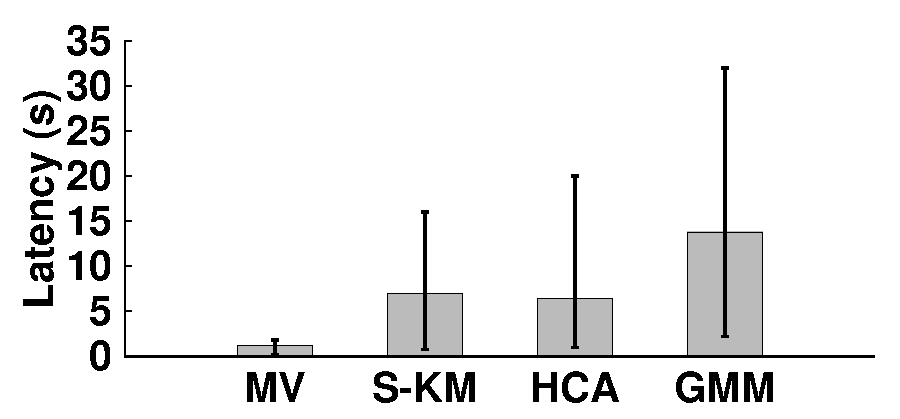
\includegraphics[width=3.0in,angle=0]{Figs/DriveSense/clustering_methods.pdf}
\vspace{0.0cm}
\caption{The time used to detect there is an orientation change.}
\vspace{-0.2cm}
\label{evaluate_latency}
\end{center}
\end{figure}


\textbf{Detection Latency}. 
Detecting orientation change timely can reduce possible inaccurate 
estimations. 
We compare the moving variance (MV) method with other common
data stream clustering method such as 
sequential K-means (SK), hierarchical clustering (HCA) 
and Gaussian Mixture Models (GMM). 
We run the four methods in 10 different orientation changes, 
and the results are shown in Fig. \ref{evaluate_latency}. 
MV can detect orientation change in 10-20 data samples (1-2s). 
The common incremental clustering techniques require more
time as it needs more data to form/detect another cluster. 



\subsection{Comparison Between GPS and IMU Sensors}

\begin{figure}[!htbp]
\begin{center}
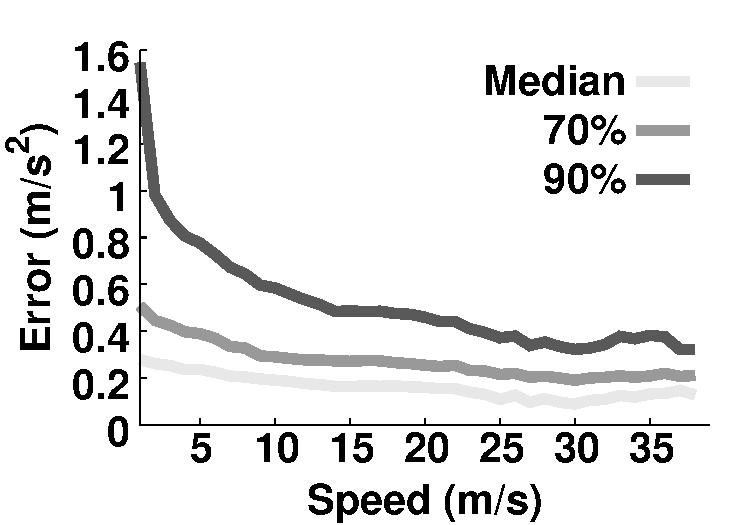
\includegraphics[width=3.0in, angle=0]{Figs/DriveSense/speed_acce_error.pdf}
\vspace{-0.2cm}
\caption{GPS acceleration estimation errors under various speeds.}
\vspace{-0.4cm}
\label{speed_acce_error}
\end{center}
\end{figure}




\begin{table}[!htbp]
        \centering
        \vspace{0.5cm}
        \caption[icv_accuracy]{Median ICV and Acceleration Estimation Accuracy}
         \vspace{0.0cm}
        \label{icv_accuracy}
                \begin{tabular}{|l|c|c|c|}
                \hline
ICV Median & Median Error & $70th-\%$ & $90th-\%$ 
\\  \hline      \hline
0.05 & $0.15m/s^2$  & $0.18m/s^2$ & $0.31m/s^2$ 
\\  \hline
0.21 & $0.21m/s^2$  &  $0.38m/s^2$ & $0.95m/s^2$   
\\  \hline
0.87 & $0.45m/s^2$ & $0.78m/s^2$ & $1.56m/s^2$   
\\  \hline
\end{tabular}
\end{table}


To select between IMU sensor and GPS as input
for acceleration estimation, 
we compare the accuracy based on current speed and 
mounting stability. 
To estimate the accuracy of GPS, 
we use one pipeline to process GPS stream data 
and track the speeds. 
Each GPS point is associated with a confidence value. 
The confidence value is the $\beta$$th$ percentile
estimation accuracy under given speed.
The percentile accuracy under various speeds
is illustrated in Fig. \ref{speed_acce_error}.
To estimate the accuracy of IMU sensors, 
we use ICV to track the mounting stability of the smartphone. 
We use the median ICV as an indicator of
the mounting stability. 
The corresponding percentile errors of different
ICV are illustrated in Table \ref{icv_accuracy}.



\subsection{Training Time}

\begin{figure}[!htbp]
\begin{center}
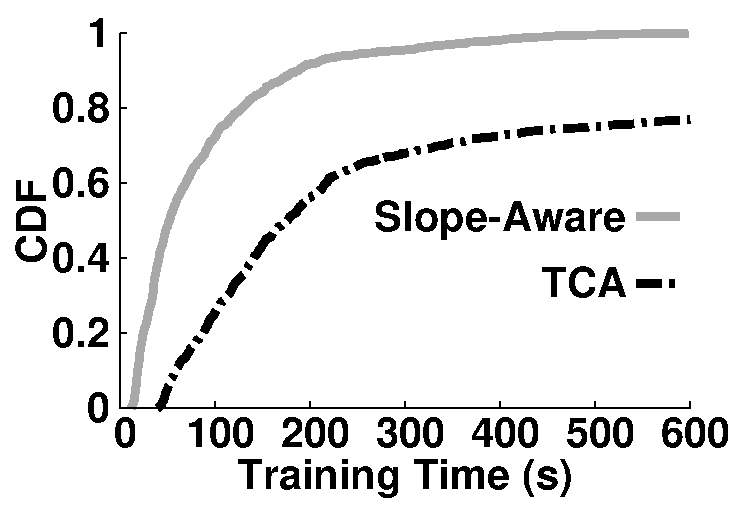
\includegraphics[width=2.8in,angle=0]{Figs/DriveSense/slopeaware/alignment.pdf}
\vspace{-0.2cm}
\caption{The training time used for coordinate alignment.}
\label{alignmenttime}
\vspace{-0.3cm}
\end{center}
\end{figure}

The training time of a coordinate alignment algorithm is critical
for real-time applications such as hard brake warning \cite{snapshot}. 
To evaluate the training time, we extract the straight road driving segments and fed them into the replay engine.
The engine stops when the accuracy of coordinate alignment is within
a predefined percentage of the accuracy when we use the segments of the entire trip to train.
As shown in Fig. \ref{alignmenttime}, 
there is a substantial improvement on the training speed.
Slope-aware alignment matrix can be trained in less than $2min$ in more than
$80\%$ of the cases, 
while it takes much longer time to train the rotation matrix if
the algorithm does not consider slope caused deviations.
The training time heavily depends on road conditions. 
For the trips with level roads and fewer bumps, it generally
takes less time to train.
On the other hand, for the trips with lots of slopes and bumps on the road, 
it takes much longer time to train due to less training opportunities.


\subsection{In the Wild}


%\subsubsection{Statistics}

\begin{figure}[!htbp]
\begin{center}
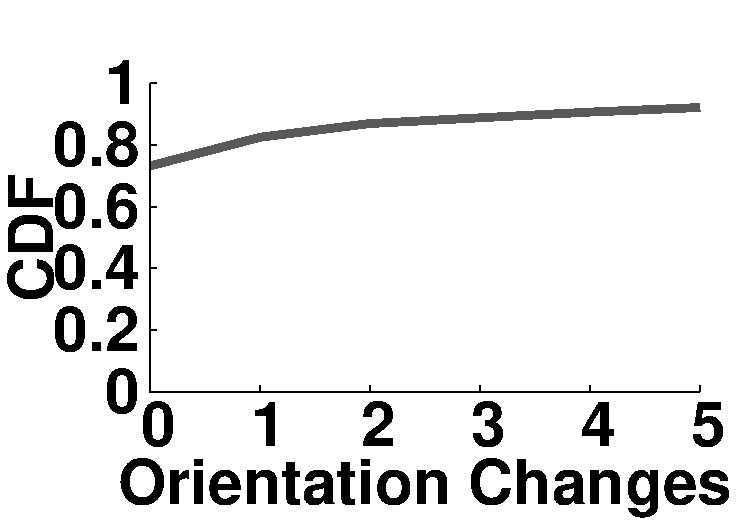
\includegraphics[width=1.7in,angle=0]{Figs/DriveSense/evaluation/wild_changes.pdf}
\hspace{-0.5cm}
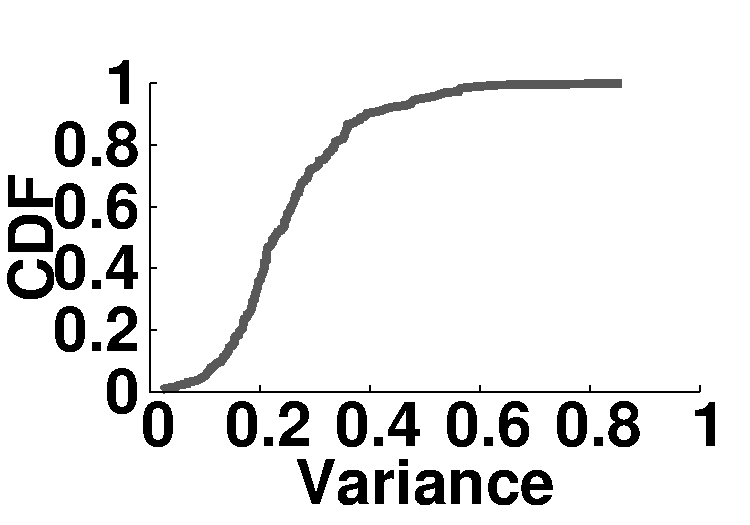
\includegraphics[width=1.7in,angle=0]{Figs/DriveSense/evaluation/wild_variances.pdf}
\vspace{0.0cm}
\caption{The orientation change and stability measurement statistics.}
\vspace{-0.2cm}
\label{wild_evaluation}
\end{center}
\end{figure}


The beta version of our Android application (the full version with 
trip upload, user management and back-end server etc.) is released to
9 volunteers for the past half year. 
There are totally 269 trips collected. 
The trip recording functionality of the app is designed as an Android 
Service, so it is able to run in the background. 
We observe some users forget to stop the app, 
so we add another functionality to stop recording if there
is no high speed movement in 10 minutes. 
The volunteers are asked to place the Android phone
at anywhere they prefer. 
Among the 269 trips we collected, 
orientation change occurs in 74 trips. 
The CDF of the orientation change statistics are 
illustrated in Fig. \ref{wild_evaluation}.
Normally it takes about several minutes to find a fragment
to train the rotation matrix, frequent changing 
the orientation may reduce the opportunities using
inertial sensors. 
We also evaluate the stability or the variance of the trips 
without orientation changes. 
The results, as shown in Fig. \ref{wild_evaluation}, 
indicate that the smartphones are mounted tightly
in most of cases. 
There are about $25\%$ trips where the smartphone is not 
tight enough (high variances) and GPS should be used instead. 


\nop{
\subsubsection{Parameter Selection}

\begin{figure}[!htbp]
\begin{center}
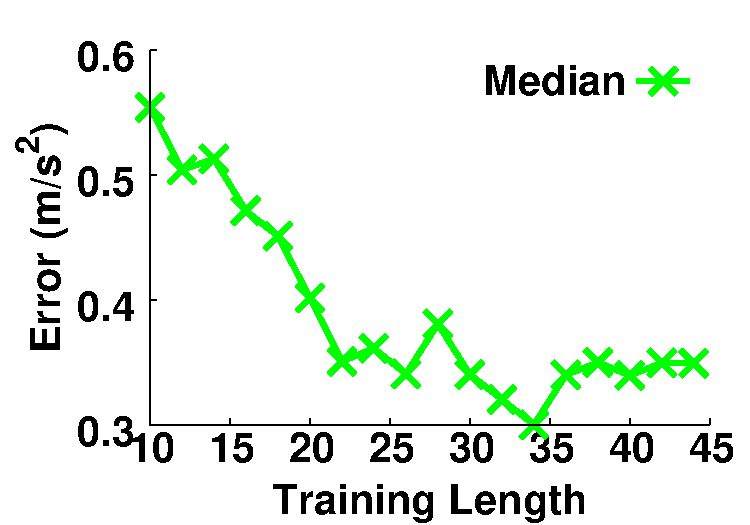
\includegraphics[width=1.7in,angle=0]{Figs/DriveSense/trainlengthanderror.pdf}
\vspace{0.0cm}
	\caption{The training length is related to horizontal alignment median error.}
\label{training}
\vspace{-0.2cm}
\end{center}
\end{figure}
}







\section{Limitation and Discussion}


\textbf{Extra Power Consumption of GPS}. 
The use of GPS will accelerate the power consumption of the smartphone. 
We believe user experience is more important
than power consumption within vehicle, 
where the user is able to charge the smartphone. 
We find that some vehicle travel recording applications, like DriveWell \cite{cmt} , monitoring GPS information
in the background. 
We believe the users are willing to enjoy some 
vehicle service such as navigation and travel recording
in exchange for some extra power.  



\textbf{Better or Worse GPS accuracy}. 
Our GPS evaluation is limited to existing techniques as well as the
geographic scope where we collected the data. 
The GPS has a chance to perform better with more advanced algorithms
or worse with signals blocked by high buildings. 
Google has implemented the API which allow the application layer to use raw GNSS data as input
since Android 7.0 system \cite{android_gnss, google_gnss_tools}.
With extra input, we believe the accuracy of GPS in commodity 
smartphone could be improved. 
The accuracy of GPS in metropolitan cities could be decreased when vehicles are passing through high buildings blocking the GPS signal.
DriveSense is a system framework that can alternatively use the best estimation
Method.
With the training and modeling techniques presented in this paper, 
we believe DriveSense is able to accommodate new techniques.  

\textbf{High-end Vehicles}. 
There are emerging selfdriving techniques that ultilize 
expensive hardwares to scan the road, 
which may provide better accuracy on road condition
monitoring. 
Also they could be equipped with built-in sensors
and alignment is not a problem anymore. 
But our techniques about linear acceleration
estimation and fusion with GPS still work
in such cases. 
We argue that the majority of existing
vehicles are still low-end vehicles 
and we expect they will still dominate 
the road in the next decade. 
Our techniques can be used in either high-end 
or low-end vehicles by using only
a single smartphone. 


\textbf{Device and Orientation Diversity}. 
We are not able to try all the devices and 
every possible orientation. 
The devices we used include Motorola Xoom,
HTC Hero, LG Nexus 5, LG Nexus 5x and Motorola Nexus 6. 
The devices are placed in the back pocket of passenger
seat, vertically /horizontally in car mount holder, 
car cup holder, passenger seat, pants pocket, 
and passenger hand.  
We believe the diversity of devices and orientations in our study are representative enough. 
We have not observed neither particular device nor 
the orientation influence on vehicle motion sensing
with inertial sensors. 






\section{Summary of DriveSense}




Smartphones are commonly used for driving analytics applications. 
Traditional approaches assume experimental
cases where the smartphone is stably mounted with fixed relative orientation
and the vehicle is travelling on flat roads. 
By using an example experiment, we show that 
even perfectly aligned accelerometer suffers acceleration overestimation or underestimation, 
which is caused by gravitational force, misalignment and slope estimation error.  
Moreover, the accuracy of IMU sensors are sensitive to human interactions
as well. 
For example, frequent relative orientation change and less stable mounting
may cause significant estimation errors. 
In this work, the defects are remedied
with following innovative techniques. 
First, a slope-aware alignment algorithms to reduce the slope influence, 
meanwhile, to improve alignment accuracy. Also, we track the linear 
acceleration of the vehicle to address acceleration over/under estimation problems. 
Second, in order to timely update 
vehicular motion parameters, the relative orientation changes of 
smartphone are detected using machine learning algorithms. 
Third, we model mounting stability of the smartphone and 
evaluate the sensing accuracy under different stability estimations.  
Fourth, we present the tradeoffs between inertial sensors, the primary sensors, 
and GPS, which is used when inertial sensors lose accuracy or disable. 
To evaluate our solutions, we compare the estimated 
accelerations with those calculated from OBD speed readings.  
The accuracy of our methods are evaluated with highway and urban traces
covered by 13,000 miles in the northwestern US.
We show through our experiments and analysis that
compared to current state of the art techniques, 
our method improves the $75$-percentile accuracy 
by $5\times$ comparing with well-tuned inertial sensors in traditional approach. 






\begin{algorithm}
\caption{Angle Search Algorithm}
\label{search}
\begin{algorithmic}[1]
\Input{$D_a$: The 2D accelerometer data after horizontal alignment}
\Output{$\theta_{o}$: The best fit angle}
\Procedure{AngleSearch}{}
\State $dev_{min} \gets MAX$;
\State $D_{t} \gets []$;
\For{$\theta$ \texttt{in} (-$\alpha$, $\alpha$)}
\For{$[y_i, z_i]$ \texttt{in} $D_a$}
\State $M_\nu$ $\gets$ $\begin{bmatrix}\cos\theta & -\sin\theta\ \\ \sin\theta & \cos\theta \end{bmatrix}$;
\State $[y'_i,z'_i]$ $\gets$ $[y_i,z_i]* M_\nu$;
\State $D_t.push(z'_i)$;
\EndFor
\State $dev_x \gets deviation(D_t)$;
\If {$dev_x < dev_{min}$}
\State {$dev_{min}$ $\gets$ $dev_x$};
\State {$\theta_{o}$ $\gets$ $\theta$};
\EndIf
\EndFor
\Return $\theta_{o}$;
\EndProcedure
\end{algorithmic}
\end{algorithm}
\vspace{-0.6cm}






%
\chapter{Improving Fuel Efficency and Reducing Carbon Emissions}


\section{Introduction}



The fuel conumption and carbon pollution caused by 
driving activities are drawing more and more attentions. 
In 2013, the White House issued a climate action plan to reduce fuel consumption
and carbon pollution \cite{whitehouse2013}. 
In the same year, Morgan Stanley reported that 
there will be \$158 billion annual savings in the US 
if all cars adopted smooth driving styles \cite{morganstanley2013}. 
We introduce a driver assistance system, called EcoDrive, 
that can improve the fuel efficiency of a vehicle's drive by sensing, computing, 
and actuating the acceleration behavior of the vehicle in an autonomous manner, 
by modeling properties of the vehicle, road conditions, and driving actions. 
With the global push for improving fuel efficiency of vehicles to 
reduce consumptions and carbon emissions, 
we believe solution such as ours can be one of many important mechanisms to meet such a goal.


\begin{figure}[t]
\begin{center}
\vspace{-0.5cm}
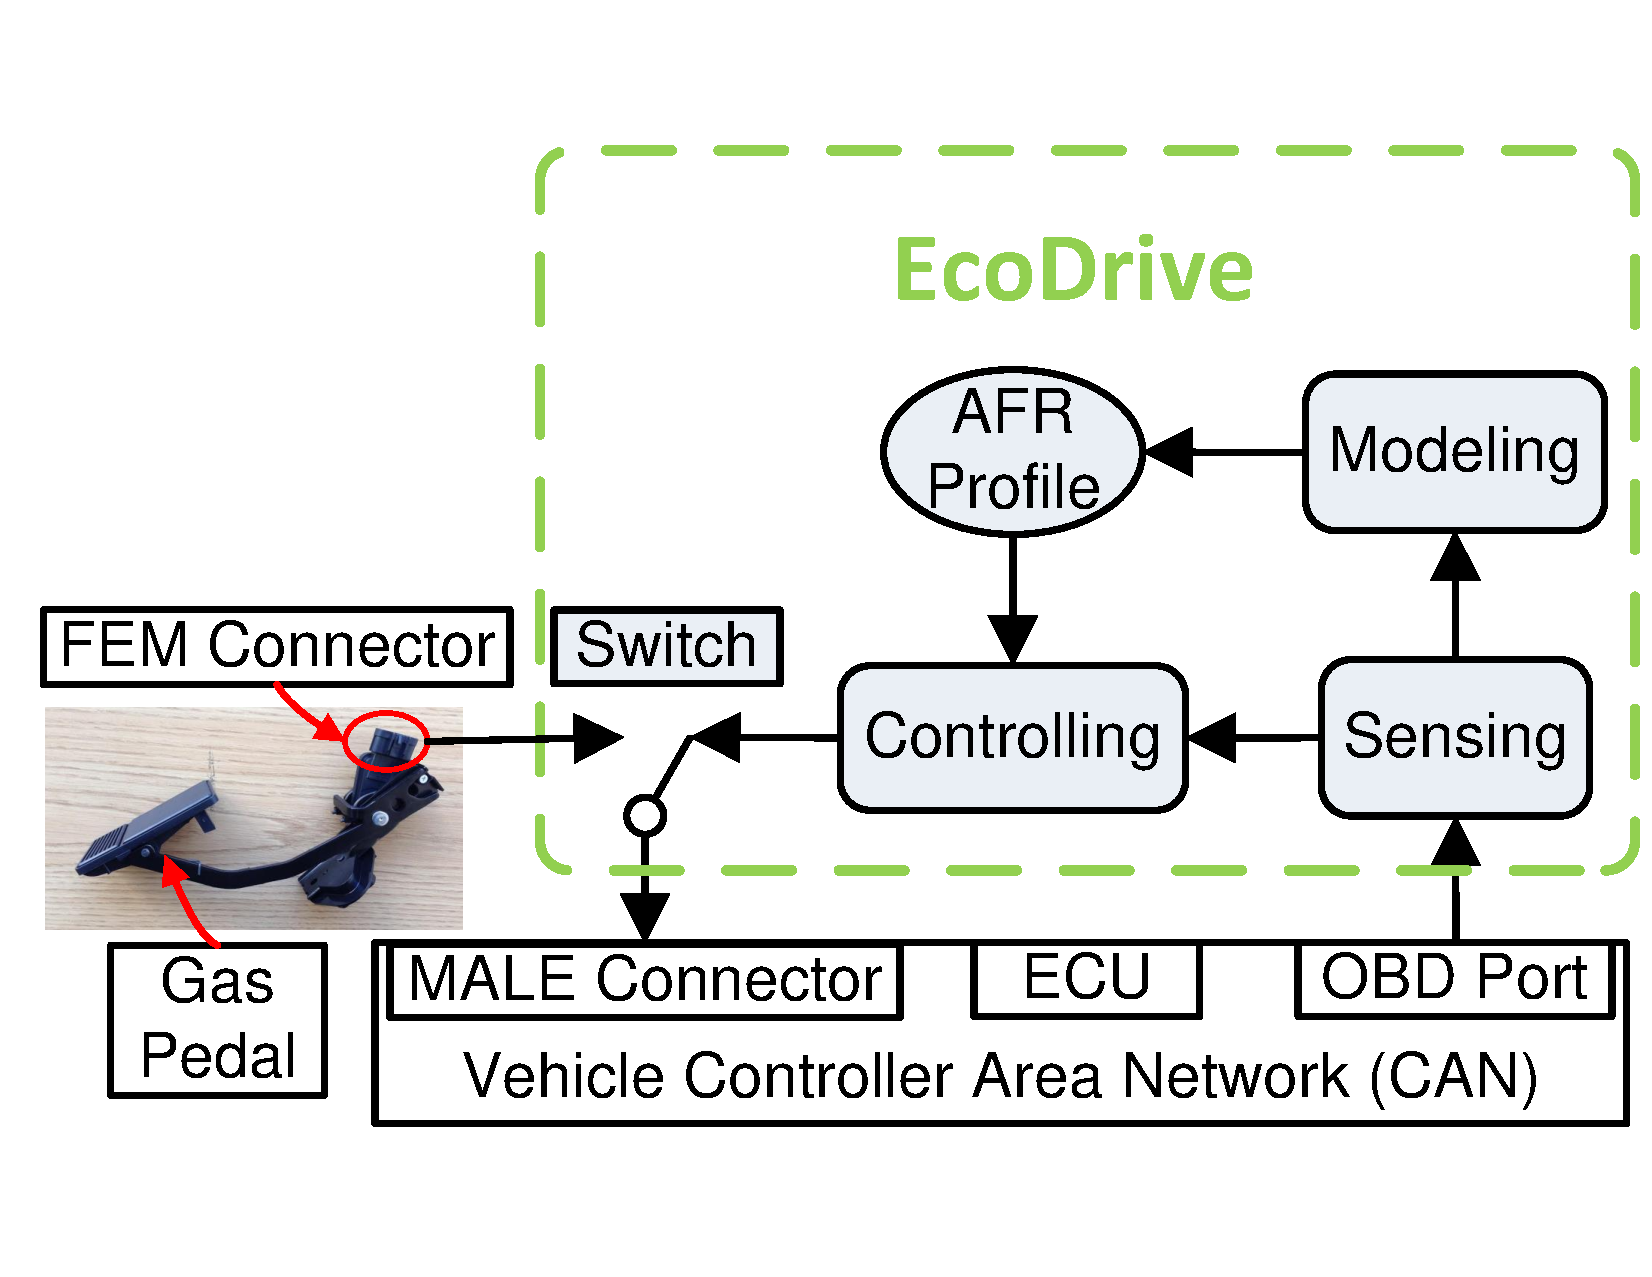
\includegraphics[width=4.0in,angle=0]{Figs/EcoDrive/architecture.pdf}
\vspace{-0.5cm}
\caption{EcoDrive Architecture.}
\vspace{-0.7cm}
\label{ecodrive}
\end{center}
\end{figure}


EcoDrive estimates instant fuel consumptions of different driving behaviors
based on sensed vehicle parameters from the On-board diagnostics (OBD) port \cite{obd, pid}. 
It can adjust vehicular speed in real time according to 
individual vehicle properties and road conditions 
to achieve higher fuel efficiency measured by Kilometer Per Liter (KPL)
\footnote{KPL refers to the distance travelled per unit volume of fuel consumed. 
It interchangeable with Mile Per Gallon (MPG), i.e., 1 KPL = 2.35214583 MPG.}.
EcoDrive is an independent system that can be installed on or removed from 
regular vehicles easily. 
This system controls the vehicle's acceleration and speed 
to provide a fuel efficient drive on its path. 
In our work and current implementation, 
we design this system assuming there is no other factors that 
would contribute to a choice of acceleration and speed, 
e.g., other vehicles, pedestrians, etc. or other obstacles in vicinity. 
Clearly in a practical system, this knowledge would be critical in modifying the acceleration behavior. 
Currently, we adopt the approach followed by other equivalent systems, 
such as cruise control \cite{cruise_control}, which allows the driver to instantly 
disable cruise control by actively pressing the brake pedal. 
In an analogous way, in our current implementation, 
we provide the driver a switch which can be pressed to instantly disable EcoDrive, 
if its acceleration behavior is perceived to be unsafe for nearby vehicles or obstacles.






\textbf{EcoDrive Components}. 
EcoDrive delivers its design via three components including an OBD sensing component, 
a vehicle dynamics modeling component and an acceleration controlling component. 
The architecture is illustrated in Fig. \ref{ecodrive}. 
The sensing component reads real-time OBD parameters through
the OBD port. 
The modeling component models various vehicle forces 
as functions of instant fuel consumption and produces
a fuel consumption profile, called Air/Fuel Rate (AFR) profile
\footnote{AFR refers to the volume of air/fuel cost per unit time.}.
The controlling component utilizes the AFR profile to calculate fuel efficient
driving strategies according to speed limit and road conditions. 
EcoDrive emulates the gas pedal by sending voltage values to 
the connector through an Arduino board.
The vehicular Electronic Control Unit (ECU) controls air/fuel injection rate
according to the voltage inputs. 

EcoDrive addresses two main challenges. 


%\textbf{How to model vehicle dynamics and build AFR profile by using OBD parameters, 
%given various vehicle types, transmission types and road conditions?}
\textbf{a) Model Vehicle Dynamics based on OBD Parameters}.
EcoDrive uses the OBD parameters delivered by
the sensing component to build an AFR profile, 
which records instant fuel consumptions of various accelerations under different speeds. 
To this end, EcoDrive models various vehicle forces, 
including propulsion, drivetrain loss, wind resistance
and grade resistance, as functions of instant fuel consumption.  
First, we model propulsion (or output torque) as a function of engine
torque and gear ratio \cite{vong2006prediction, giannelli2005heavy}. 
We use AFR to model engine torque, and use the ratio between RPM
and vehicular speed to model gear ratio. 
Second, we represent drivetrain loss and wind resistance as a function
of vehicular speed \cite{andersson2012online}.
The coefficients are estimated from recorded data traces where
the car is driving at constant speeds. 
The basic idea is that the sum of resistances is equal to
propulsion when the car is driving at a steady-state speed. 
Third, we model grade resistance by altitude changes over road segments. 
The altitudes of the locations are obtained from 
National Elevation Dataset \cite{nationalelevation}.   
Based on the three models, AFR is modeled as a function of 
speed, acceleration and road conditions. 


\textbf{b) Control Air/Fuel Rate and Vehicular Speed to Improve Fuel Efficiency}.
%\textbf{How to control accelerations and cruising speeds to improve
%gas mileage, given various road segment lengths and speed limits?}
EcoDrive controls vehicular speed by emulating gas pedal. 
It sends the emulated gas pedal position values to the
Arduino board which then converts the position
values to corresponding output voltages.
The output voltages are delivered to the ECU through a 6 Pin Connector.  
The problem is how to adjust vehicular speeds to travel through
a certain distance with the lowest fuel consumption.
We solve this problem by using dynamic programming. 
Each state of the dynamic programming model records 
the minimum air/fuel cost that allows the car to achieve
the current speed at the current location. 
In this model, speed can only increase and the last state of each
speed records the minimum fuel consumption if the car reaches the pre-assigned distance at that speed. 
We call the speed with minimum fuel consumption the target speed.  
By backtracking the state matrix from the last state
of target speed, EcoDrive can obtain the desired AFR at each speed. 
EcoDrive adjusts air/fuel injection rate based on real-time sensed vehicular speed. 
Once the vehicular speed reaches the target speed, EcoDrive
enters a cruising state and commands a constant air/fuel injection rate
until the car reaches the pre-assigned distance. 



\textbf{EcoDrive Prototype}. We build a prototype of EcoDrive in an off-the-shelf mobile embedded platform. 
The prototype is installed and tested on a 2011 Chevrolet Impala. 
We test EcoDrive on the Impala for more than 100 miles in both urban and highway environments.
We evaluate the fuel consumption of EcoDrive and human drivers on different road segments.   
In urban areas, EcoDrive achieves 10\%-40\% higher fuel efficiency than four recruited human drivers.
On highway, we evaluate EcoDrive on two highway segments with different target speeds.    
In our user tests, EcoDrive has over 30\% improvements compared to different human drivers. 
In comparison with cruise control, which is more fuel efficient
than human drivers in the traces we collected, 
EcoDrive achieves an average of 10\% higher fuel efficiency.  
We evaluate the performance of EcoDrive on other vehicles by using trace-driven simulation
based on the 10,000 miles data collected from 12 different vehicles. 
We further find that instant
fuel economy display on regular vehicles is misleading and cruise
control is fuel consuming during speed changes (either requested
by user or affected by road conditions).  






\section{Preliminaries}





To illustrate how vehicle system works 
and how each components are related to different OBD parameters,
we present a high-level vehicle system control 
flow in Fig. \ref{vehicle_system}. 
Drivers accelerate vehicle by pressing the gas pedal, 
and then the gas pedal position will be sent to 
the Electronic Control Unit (ECU). 
The ECU controls air/fuel injection rate
to produce engine torque to drive the vehicle.   
Transmission is used in this process 
to transit power from engine to wheel and 
match engine rotational speed with wheel rotational speed. 


\begin{figure}[t]
\begin{center}
\vspace{-0.0cm}
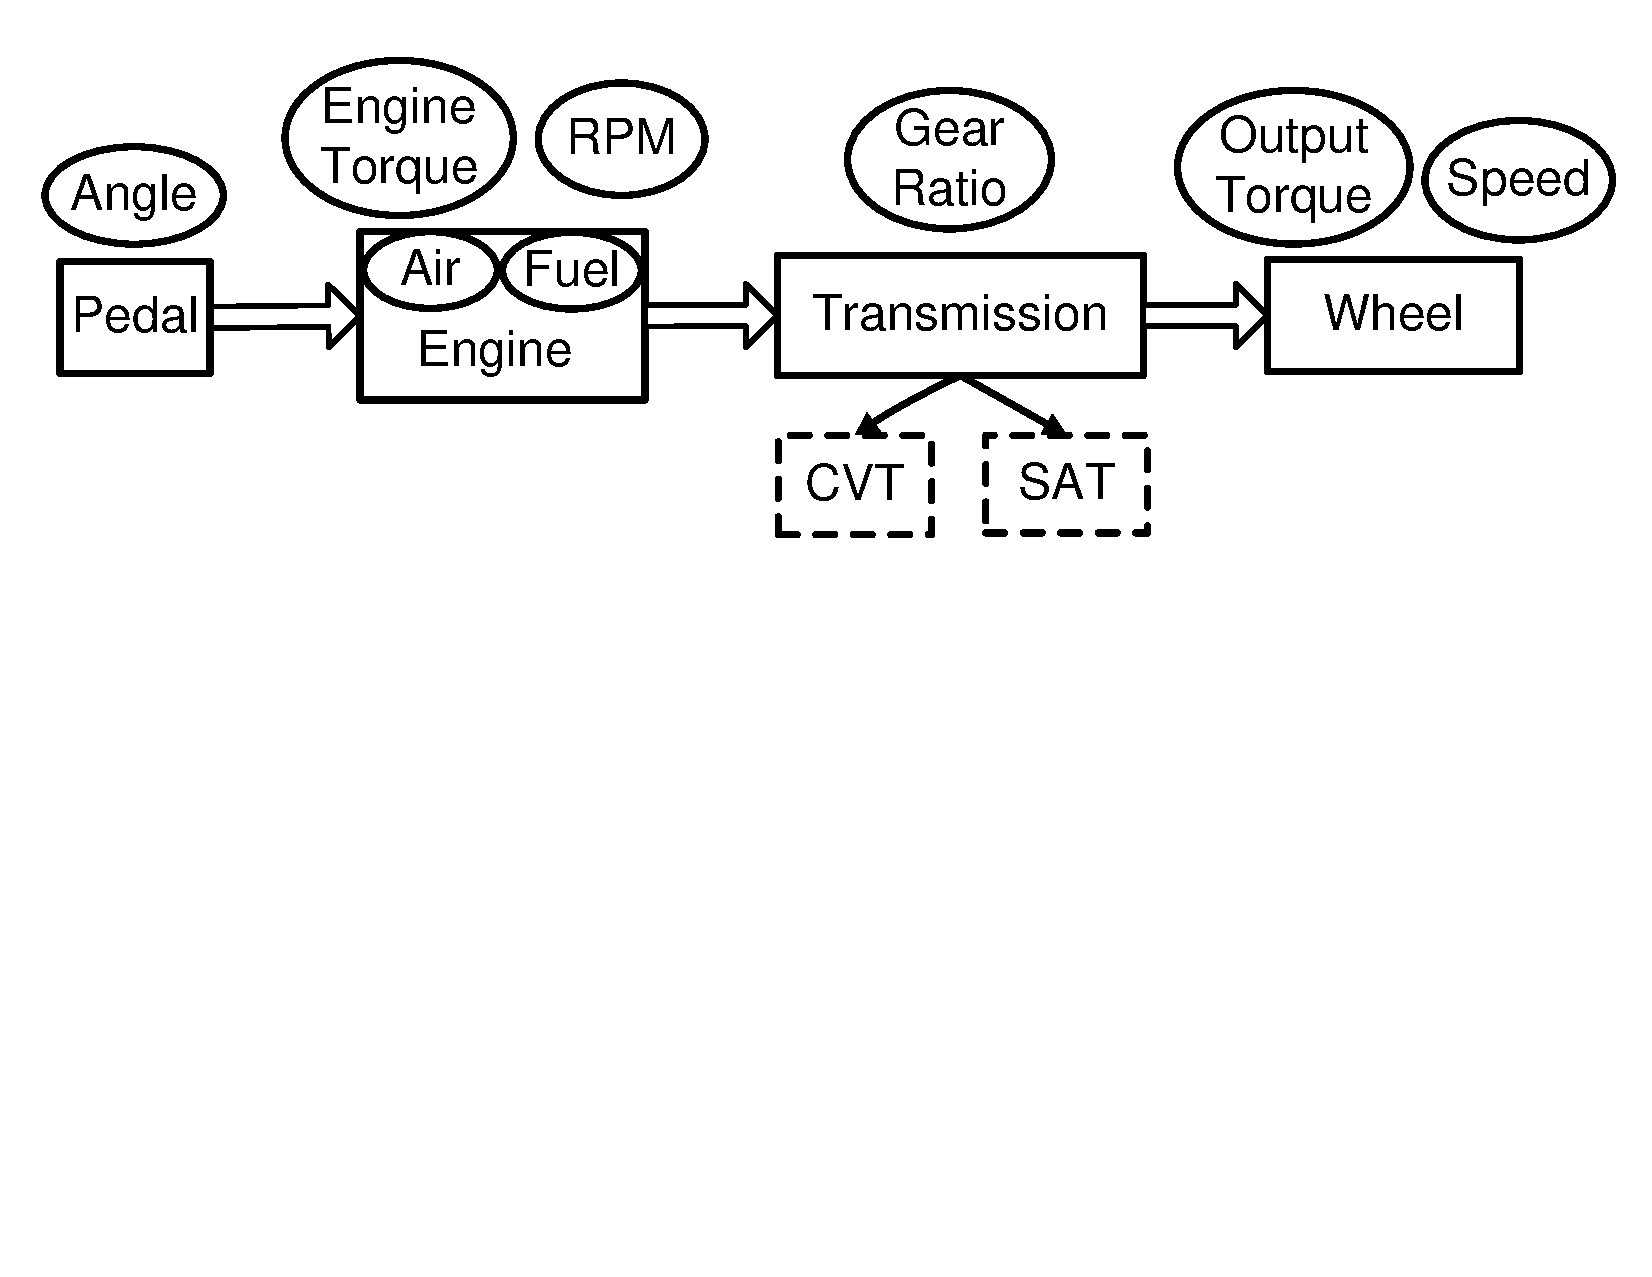
\includegraphics[width=5.0in,angle=0]{Figs/EcoDrive/drivetrain.pdf}
\vspace{-5.5cm}
\caption{Vehicle Drivetrain.}
\vspace{-0.5cm}
\label{vehicle_system}
\end{center}
\end{figure}


\subsection{Power Production and Transition}

In a car engine, the explosion of compressed fuel and air 
produces the power to drive a car.
The air is injected through an intake port and expelled from an exhaust port.
The volume of oxygen in the exhaust air is monitored by fuel trim sensors. 
Based on fuel trim sensor readings, the Electronic Control Unit (ECU) 
calculate the desired fuel injection rate to maintain the
ideal air/fuel ratio 
\footnote{Air/fuel ratio is a constant value around 14.67, 
while air/fuel rate is the volume of air/fuel injected per unit time.}. 


The burning of air and fuel mixture triggers the revolution of 
crankshaft, which carries piston power out of the engine to the transmission.
The transmission carries power to wheels.  
Transmission is also known as gearbox that uses gears and gear trains
to provide speed and torque conversion. 
The transmission reduces the higher engine speed to the slower
wheel speed and increases torque in the process of accelerating the vehicle. 
The transmission converts engine revolutions to driveshaft revolutions, and then to axle revolutions.
A Continuously Variable Transmission (CVT) is a 
transmission that can change 
seamlessly through an infinite number of effective gear ratios 
between maximum and minimum values. 
This contrasts with Step 
Automatic Transmissions (SAT) that offer a fixed number of gear ratios.

\subsection{OBD Parameters}

On-board diagnostics (OBD) is an automotive 
term referring to a vehicle's 
self-diagnostic and reporting capability.  
It is the interface between car Controller Area Network (or CAN bus) and external devices, 
e.g., a OBD scan tool that connects the OBD port and a laptop. 
Car CAN bus allows vehicular components to communicate with each other. 
For example, a position value is sent to 
the Electronic Control Unit (ECU) after human driver
press the gas pedal, 
and the ECU adjusts air/fuel injections according to the position value.
Therefore, we can read this position message transmitted over CAN bus 
from the OBD port. 





The data we collected from the OBD port are summarized in Table \ref{obd_data}. 
Fuel Level (FL) of the vehicle is usually measured by a float sensor, 
which is usually visualized on the fuel gauge in the car \cite{fuel-gauge}.
The FL is calculated according to the height of the float. 
\nop{
When fuel is injected into the tank, the fuel will raise 
the float up, and vice versa. 
This mechanism makes the FL measurement is not accurate
and can be only used to long-term fuel consumption estimation. 
For example, the float may reach the top of the tank even 
before the tank is filled up.
The fuel gauge will show a full tank even 
when more fuel is possible to be filled.  
Similar thing happens when the fuel tank close to empty. 
}
The Fuel System Status (FSS) is used to indicate current engine mode, 
open loop mode or closed loop mode. 
In open loop mode, 
the engine calculate the fuel injection based on the pre-calculated
table and there is no feedback to the engine to adjust the fuel injection rate. 
The engine runs in open loop mode during short warm up time
and runs in closed loop mode at most of the time. 
In closed loop mode, the engine adjusts fuel injection rate based on
fuel trims and air flow rate. 
Mass Air Flow Rate (MAF) is used to measure the air intake rate of the engine, 
and therefore an effective indicator of instant fuel consumption 
\cite{alessandrini2012consumption, lee2011estimation, koukoumidis2011signalguru}. 
Both Long Term Fuel Trim (LTFT) and Short Term Fuel Trim (STFT) are used to 
adjust the air/fuel rate injected into engine. 
LTFT changes less frequent than STFT. 
We use AFR as a metric of 
instant fuel consumption and/or carbon emission. 


\begin{equation}
AFR = C_f * MAF * (1 + LTFT) * (1 + STFT).
\end{equation}

where $C_f$ is a constant value for unit conversion, e.g., from air flow rate to
fuel rate or to carbon emission rate. 

Vehicular Speed is measured by the perimeter of the wheel and 
number of rotations. 
Accelerator Position is measured by the angle of the gas pedal.
It controls the air/fuel rate injected into the Engine.  
Engine RPM is measured by the rotation speed of the engine motor. 


\subsection{Dataset}



\begin{figure}[t]
\begin{center}
%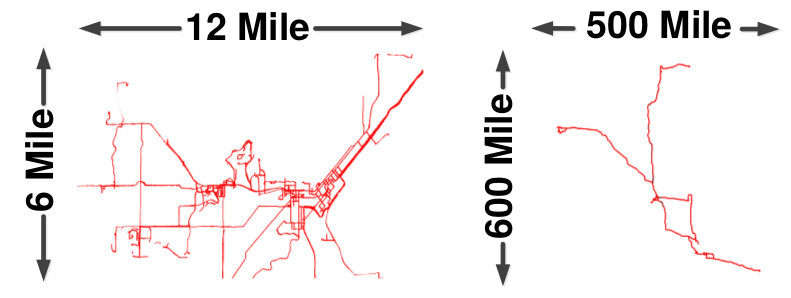
\includegraphics[width=3.0in, angle=0]{Figs/EcoDrive/urbanhighwaymap.png}
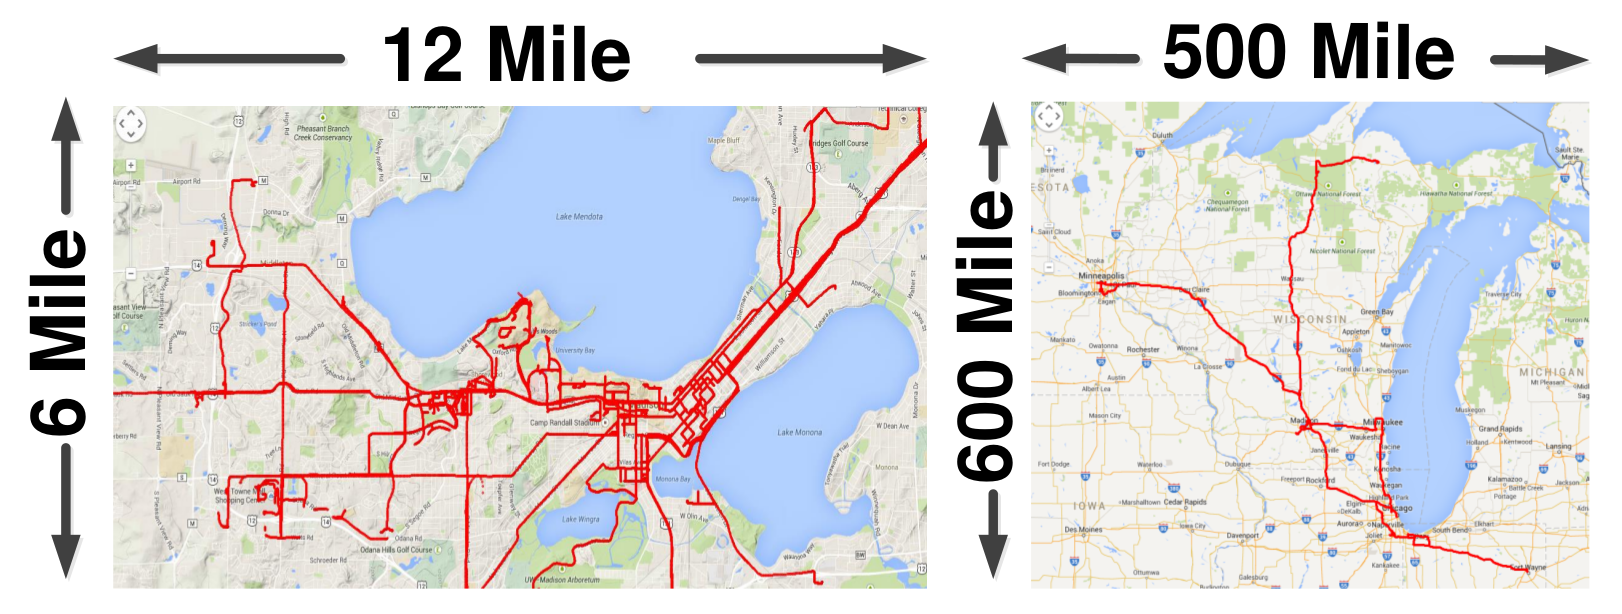
\includegraphics[width=5.0in, angle=0]{Figs/EcoDrive/map.png}
\vspace{-0.0cm}
\caption{Urban driving data (left) is collected from a US mid-size city.  
Highway driving data (right) is collected from both local highways and cross-state highways.}
\vspace{-0.5cm}
\label{rpm_gph}
\end{center}
\end{figure}


%The map area is about 600 mile $\times$ 500 mile.
%The map area is about 6 mile $\times$ 12 mile. 


We use a customized Android application to collect OBD and GPS data 
from different car makes and models.
The dataset is summarized in table \ref{vehicles}.
The transmission of car 2,6,9,10 and 11 is CVT and the rest is SAT. 
The driving data of car 1-6 is collected over a course of three months, 
and the rest is collected from random events, 
e.g., three cross-state highway trips are collected by car 7, 8 and 9, 
respectively. 
Here we separate urban driving and highway driving,
as urban driving patterns are dominated by frequent 
accelerations and decelerations while 
highway driving patterns are dominated by 
constant speed cruising. 
The dataset covers car makes from three different countries, 
urban data over 5,000 miles, highway data across 5 US states and 
over 5,000 miles, two common types of transmissions. 
We use the first car to install a prototype of EcoDrive and tested
it in both urban and highway environments. 
%EcoDrive is tested on Madison's West Betline Highway, between exit 257 and 261. And US 14 Highway between exit 132 and 136.




\subsection{EcoDrive Architecture}

EcoDrive reads real-time OBD parameters through OBD port
and controls air/fuel injection rate by emulating the gas pedal.
We illustrate the architecture of EcoDrive in Fig. \ref{ecodrive}.
The sensed parameters from OBD port are passed to modeling component
to train the models.
The modeling component builds an AFR profile to 
record the instant fuel consumptions of various 
accelerations at different speeds.
Based on pre-calculated driving strategy and real-time sensed vehicular speed, 
the controlling component controls air/fuel injection rate to adjust vehicular speed by 
sending the gas pedal position values to the ECU. 
To emulate the gas pedal, we utilize the drive-by-wire technology, 
where the gas pedal and throttle are connected by electronic messaging instead of mechanical linkage.   
It enables the position of gas pedal can be sent as a message
to control throttle position. 
The throttle controls the volume of air flow injected into the engine. 
 


\subsection{Applications}

EcoDrive is used as an independent system that can be installed
on regular vehicles.  
It can be used as a control system in a way similar to 
cruise control \cite{cruise_control, bengtsson2001adaptive, ioannou1993autonomous}. 
In this application, it is used as a EcoDrive mode that a human driver
can switch it on or off. 
Drivers are required to press the brake pedal to turn this mode off
to keep safe distance to front car or traffic lights/signs accordingly.
This mode can be integrated with intelligent front object or traffic light detection
systems \cite{bengtsson2001adaptive, ioannou1993autonomous} 
to further enhance driving experience. 
EcoDrive requires two inputs, the speed limit and road length. 
The speed limit can be specified by human driver or obtained from online database \cite{speedlimit}. 
The road length can be calculated by a navigation software.



It can also be used as a subsystem of autonomous driving systems 
\cite{googledriverlesscar, urmson2008autonomous, litman2013autonomous, kim2013towards}. 
We envision a highly autonomous and intelligent system that all the route
information are pre-calculated, e.g., speed limit, traffic conditions and
distances of each road segment etc. 
EcoDrive can be used as a subsystem to predict fuel consumption
of possible routes \cite{ganti2010greengps} and 
calculate the optimal driving strategy.  





\section{Vehicle Dynamics and Fuel Consumption}




EcoDrive models various forces as functions of instant fuel consumption and produces fuel consumption profile as output. 
Different from Existing vehicle dynamics models \cite{koprubasi2008modeling},  
we only use parameters available from OBD instead of assuming 
the engine parameters are known in advance. 
We consider several factors that affect car fuel
consumption, e.g., engine torque, 
drivetrain loss, wind resistance and grade resistance.   
The vehicle force can be modeled as follows. 

\begin{equation}
F = F_p - F_l - F_g - F_w.
\end{equation}

where $F_p$ refers to the propulsion caused by car engine, 
$F_l$ refers to the drivetrain loss caused by transmission and various gears 
connecting engine and wheels,
$F_w$ refers to the wind resistance,
$F_g$ refers to the grade resistance. 
Since we are only interested in fuel consumption on acceleration
and cruise, we exclude the forces caused by brake. 

We model the forces in the following steps.  
First, we use RPM and vehicular speed to model gear ratio and use 
AFR to model engine torque. 
Second, the drivetrain loss and wind resistance is modeled as
the counterforce of propulsion when the car is driven in constant speeds. 
Finally, we use driving data extracted from flat road to 
train the parameters of our propulsion and 
loss models, and then use the propulsion model
to model grade resistance.




\begin{figure*}[t]
\begin{center}
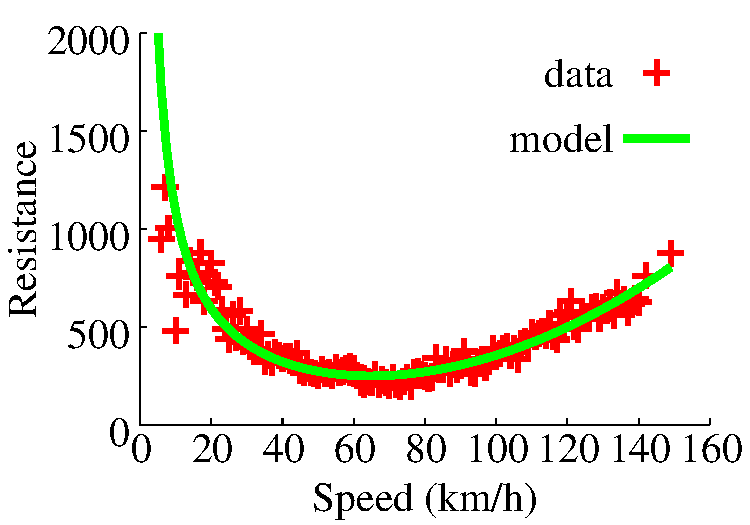
\includegraphics[width=1.8in,angle=0]{Figs/EcoDrive/lei_loss.pdf}
\hspace{-0.0cm}
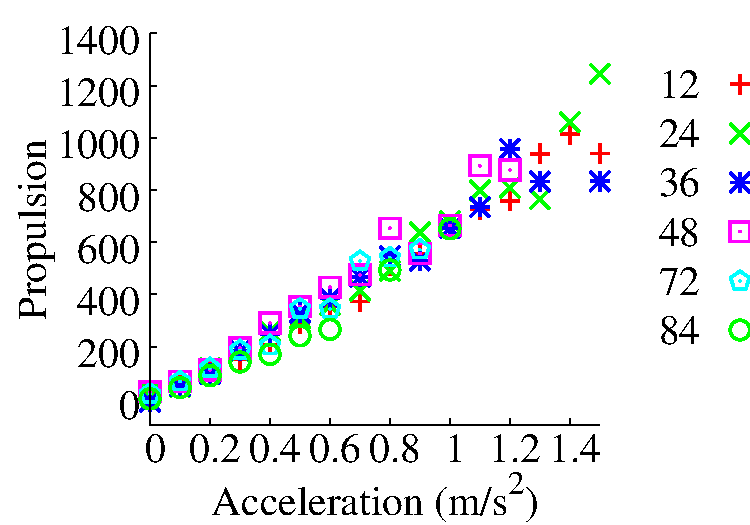
\includegraphics[width=1.8in,angle=0]{Figs/EcoDrive/lei_torque.pdf}
\hspace{-0.0cm}
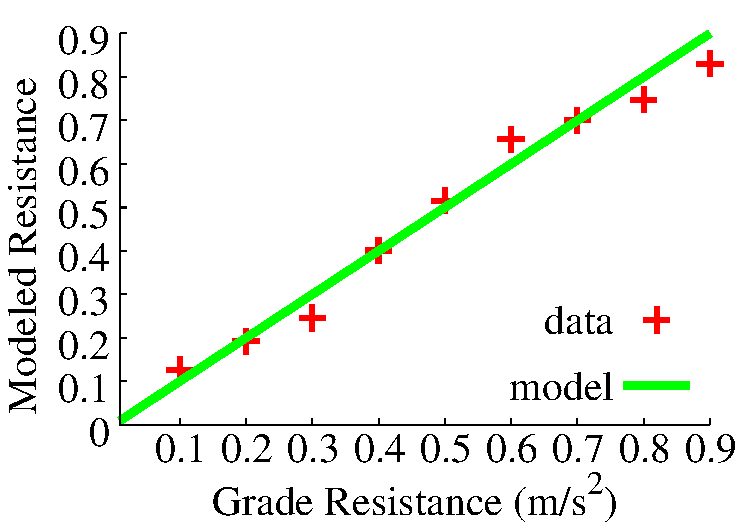
\includegraphics[width=1.8in,angle=0]{Figs/EcoDrive/lei_slope.pdf}
\hspace{-0.0cm}
\vspace{-0.2cm}
\caption{Vehicle Dynamics Modeling. The Figs/EcoDrive are about drivetrain loss and wind resistance under each speed (left), 
relation between acceleration and propulsion (minus wind resistance and drivetrain loss) under each speed (middle), 
modeled grade resistance with groundtruth (right).}
\vspace{-0.8cm}
\label{modeling}
\end{center}
\end{figure*}

\subsection{Propulsion Modeling}


The propulsion (or output torque) of vehicle is closely related
to transmission gear ratios and engine torque \cite{vong2006prediction, giannelli2005heavy}. 
The propulsion produced by vehicle engine
can be represented by

\begin{equation}
 F_p = a_p * \tau_e * R_G.
\end{equation}

where $\tau_e$ refers to the engine torque, 
$R_G$ refers to transmission gear ratio
and $a_p$ is the coefficient used for unit conversion. 


\subsubsection{Gear Ratio Modeling}

Modern vehicles are usually using automatic transmission and 
freeing the driver from shifting gears manually. 
There are mainly two types of transmissions, 
Step Automatic Transmission (SAT) and Continuously Variable Transmission (CVT). 
SAT uses discrete transmission gear ratios while CVT has an
infinite number of effective transmission gear ratios. 
Since different transmission types show different
properties of gear ratio changes over different speeds, 
we use gear ratio changes to identify different
vehicle transmission types. 
We estimate gear ratios by using RPM and speeds 
when the car is driving in constant speeds. 



In a SAT vehicle, $R_G$ are discrete values.
  
\begin{equation}
   R_G = R_i = \frac{RPM}{v}  \hspace{1cm} i = 1,...,n
 \end{equation}

where $v$ represents the vehicular speed 
and $n$ is the number of gears of a transmission, 
e.g., $n=4$ for a 4-speed transmission. 

In a CVT vehicle, $R_G$ changes continuously over time and always
approach the optimal $RPM$. 

\begin{equation}
   R_G =
   \begin{cases}
   \frac{RPM_a}{v}     &  \mbox{if} \hspace{0.2cm} v < v_T, \\
   R_b   &  \mbox{if} \hspace{0.2cm} v \geq v_T.
   \end{cases}
  \end{equation}

where $RPM_a$ is the optimal $RPM$ of a given engine, 
and $v_T$ is the speed threshold. 
If the vehicular speed is lower than $v_T$, 
the engine $RPM$ converges to a constant value $RPM_a$ under
different speeds. 
If the vehicular speed is higher than or equal to $v_T$, 
the gear ratio is a constant value $R_b$. 


\subsubsection{Engine Torque Modeling}


\nop{
\begin{figure}[t]
\begin{center}
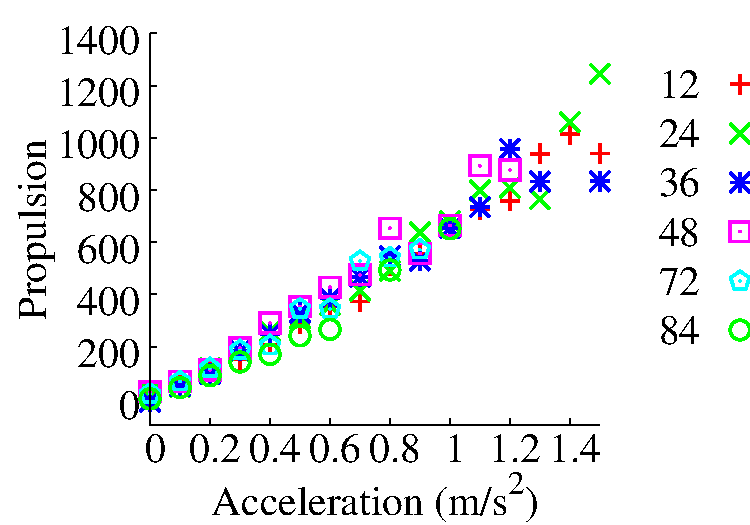
\includegraphics[width=3.0in,angle=0]{Figs/EcoDrive/lei_torque.pdf}
\vspace{-1.0cm}
\caption{Propulsion (output torque) under different speeds (km/h)
and accelerations.}
\vspace{-0.3cm}
\label{speed_propulsion}
\end{center}
\end{figure}
}

Engine torque is produced by the explosion of air and fuel, 
therefore, we can use AFR to model engine torque. 

\begin{equation}
\tau_e = AFR^{f(v)}.
\end{equation}


where $f(v)$ is a parameter function that is monotonically increasing
with vehicular speed. Based on our empirical observation, 
it starts from 0.3 at speed 0 and converges to 1 when the speed
is larger than $20km/h$. 

Therefore, the propulsion of a car on the wheel can be written as 

\begin{equation}
 F_p = a_p * \tau_e * R_G = a_p \frac{AFR^{f(v)} * RPM}{v}.
\end{equation}



\subsection{Drivetrain Loss and Wind Resistance Modeling}

\nop{
\begin{figure}[t]
\begin{center}
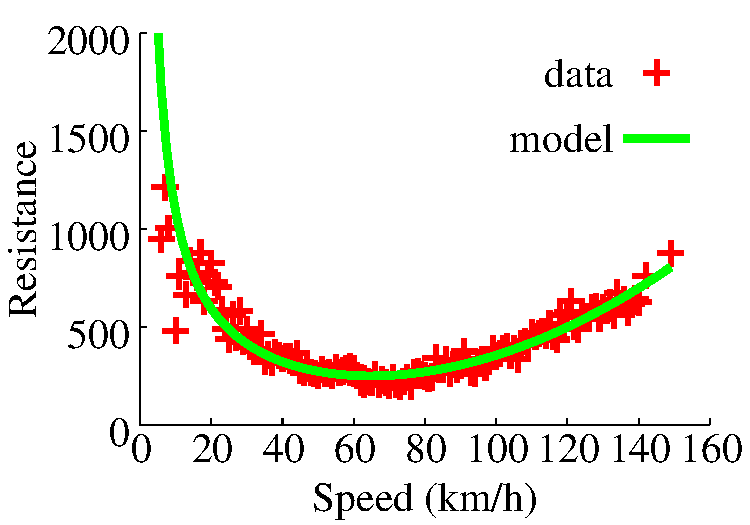
\includegraphics[width=2.4in,angle=0]{Figs/EcoDrive/lei_loss.pdf}
\vspace{-0.3cm}
\caption{Drivetrain loss and wind resistance under different speeds.}
\vspace{-0.3cm}
\label{speed_loss}
\end{center}
\end{figure}
}

Instead of modeling each loss individually, we model all the power losses
as a whole. 
There are mainly two power losses in automotive systems, 
drivetrain loss and wind resistance. 
Drivetrain loss consists of transmission loss and other mechanical system losses.  
Transmission connects car engine and wheels by various gears and
power loss occurs when transmit the power from engine to wheels. 
We model drivetrain loss in the following form.

\begin{equation}
F_l = \frac{a_l}{v} + b_l * v + c_l. 
\end{equation}

where $v$ is the vehicular speed and the rest are coefficients. 
The drivetrain loss drops to minimum when the car is driving
in moderate speed. 


The force from the air drag \cite{andersson2012online} 
can be represented by following equation,

\begin{equation}
 F_w = 0.5 * \rho_a * c_d * A_a * v^2 = a_w * v^2.
\end{equation}

where $\rho_a$ is the air mass density, 
$c_d$ is the air drag coefficient and 
$A_a$ is the effective area of the vehicle. 
Since the effective area of vehicle is different
from vehicle to vehicle, 
we model air drag as a function of vehicle speed
with unknown coefficient $a_w$. 


After we put drivetrain loss and wind resistance together, 
the modeled loss and actual loss are shown in the Fig. \ref{modeling}. 
In low speed, the main loss comes from drivetrain loss due
to mechanical frictions. 
In high speed, the main loss comes from wind resistance due to air compression. 
After we have drivetrain loss and wind resistance, 
we use propulsion minus the loss ($F_p - F_l - F_w$) to model the relation
between acceleration and propulsion, as shown in the middle of Fig. \ref{modeling}. 
For accelerations, we use extra $MAF$ instead of raw $MAF$ readings from 
the OBD port. 
Raw $MAF$ minus the $MAF$ required to maintain a certain speed is
the extra $MAF$ for this speed. 

\subsection{Grade Resistance Modeling}


\nop{
\begin{figure}[t]
\begin{center}
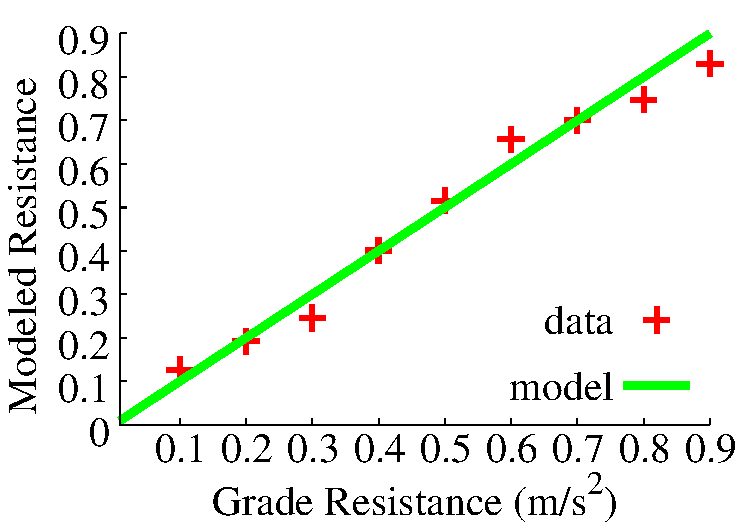
\includegraphics[width=2.5in,angle=0]{Figs/EcoDrive/lei_slope.pdf}
\vspace{-0.3cm}
\caption{Grade resistance.}
\vspace{-0.3cm}
\label{grade_resistance}
\end{center}
\end{figure}
}

Different road types, i.e., flat road, uphill and downhill, 
have significant different impacts on vehicle movements and
fuel consumptions. 
Similar to \cite{andersson2012online}, 
the grade resistance can be modeled as a combination
of forces caused by grade and rolling resistance.
\nop{
Since rolling resistance is a linear function of speed, 
so we combine it with wind resistance and focus on
grade resistance only. 
}
\begin{equation}
    F_r = mgc_r\cos{\theta}.
 \end{equation}
 
where $c_r$ is the grade resistance coefficient, 
$m$ is the vehicle mass, $g$ is the gravity of earth
, $\theta$ is the road grade and $v$ is vehicular speed.
The road elevation information is obtained from
National Elevation Dataset \cite{nationalelevation}. 
\nop{
The dataset provides fine-grained GPS elevation.
We compared the elevation dataset with Google Elevation
API \cite{googleelevation} on some routes,
and the results show that both datasets show similar accuracy. 
}




\subsection{AFR Profile}

Vehicle needs different air/fuel injection rate to achieve
different accelerations under different speeds. 
Based on the vehicle dynamics models we built in 
previous sections, we can build a fuel consumption profile. 
In this profile, we can lookup the AFR required to accelerate
a vehicle with an arbitrary acceleration under any speed. 
Let $AFR(v, a)$ denotes the air/fuel rate is required to 
accelerate the vehicle at acceleration $a$ when the vehicle
is driving at speed $v$. 
The profile can be represented as the following equation. 


\begin{equation}
AFR(v, a) = e^{\frac{log(a/R_G)}{f(v)}} + AFR_c(v)
\end{equation}


\begin{figure}[!htbp]
\begin{center}
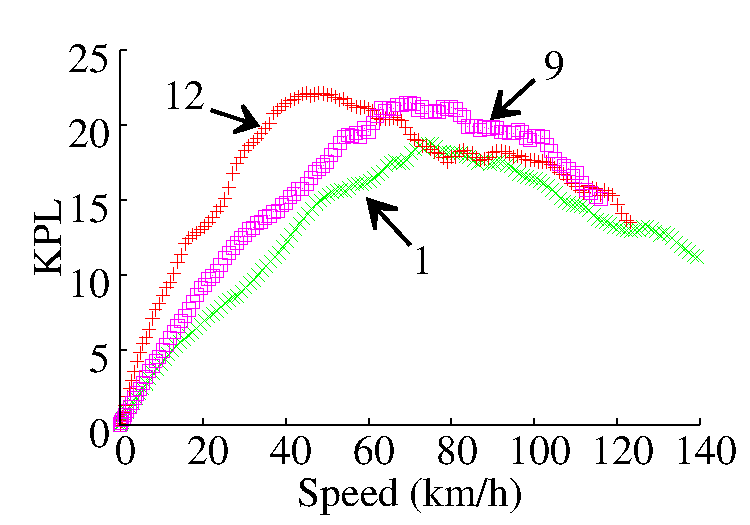
\includegraphics[width=3.0in,angle=0]{Figs/EcoDrive/speed_kpl.pdf}
\hspace{-0.4cm}
\includegraphics[width=3.0in,angle=0]{Figs/EcoDrive/acce_afr.pdf}
\hspace{-0.4cm}
\vspace{-0.3cm}
\caption{AFR profile.}
\vspace{-0.5cm}
\label{profile}
\end{center}
\end{figure}

An illustration of AFR profile of car 1 is shown in
the right subfigure of Fig. \ref{profile}. 
The profile provides the AFR required to accelerate the car
at a certain acceleration under a certain speed. 
We can infer a lookup table for each $AFR(v, a)$ based
on the profile. 
The left subfigure in Fig. \ref{profile} illustrates different
vehicles have different speed-KPL matching, 
which indicates AFR profile needs to be built
based on individual vehicles. 




 







\section{Acceleration Control}



EcoDrive controls air/fuel injection rate to control vehicular speed 
by emulating gas pedal. 
EocDrive calculates accelerations of each speed and leaves
brake decision to drivers or other systems. 
It needs two inputs, road speed limit and segment length. 
The speed limit can be set by human drivers or queried from online database \cite{speedlimit}. 
The road segment length can be estimated by human drivers or
by a third-party navigation software. 
Road segment length is not necessary for long distance roads, 
as the driving strategy will be the same if the distance is longer than
a threshold.
For example, if the speed limit is $25mph$, 
the fuel efficient acceleration strategies for $300m$ and $500m$ are the same. 
We assume both speed limit and road segment length are known. 
The output of EcoDrive is a matrix and each element in the matrix is the minimum
fuel consumption when the car arrives at a certain distance with a certain speed. 
By traversing all the possibilities, EcoDrive is able to find all reasonable
driving strategies with different fuel consumption and travel time. 


\subsection{Problem Statement}

Driving pattern can be abstracted as accelerate-cruise-brake.  
EcoDrive focuses on the accelerate-cruise part and 
leaves brake decision to human drivers. 
For example, in a $300m$ road segment with speed limit $25mph$ (or $40km/h$), 
the EcoDrive accelerates and cruises to $200m$ and 
the driver uses the rest $100m$ to stop the car as
there is a stop sign at the end of the road. 
Similar to cruise control, we assume there is enough distance
to front obstacles for drivers to brake.


EcoDrive needs two key inputs: 1) The length of the road segment, 
i.e., from current location to the point driver will make a brake, 
2) The lower and upper speed limits of the road segment. 
Such inputs can be given by user or extracted from online databases and navigation
softwares.
We focus on how to utilize such inputs to calculate
fuel efficient strategies.  
Therefore, the problem that EcoDrive is going to address can
be stated as follows:
\emph{Given a road segment length with lower and upper speed limits,
how to control air/fuel injection rate in real time to achieve the most fuel efficient driving strategy}.  


\subsection{Driving Strategy by Dynamic Programming}


\nop{
\begin{table*}[t]
        \centering
        \caption[symbols]{Notations used calculate fuel efficient driving strategy}
         \vspace{0.5cm}
        \label{symbols}
                \begin{tabular}{|l|l|}
                \hline
Symbol & Meaning 
\\  \hline      \hline
$v_i$ & The $i$th speed of the vehicle  
\\  \hline 
$a_j$ & The $j$th acceleration of a given speed 
\\  \hline
$D$ & The travel distance of the road  
\\  \hline
$d_k$ & The $k$th road segment, $D = \sum{d_k}$      
\\  \hline
$s(i, k)$ & A state represents that the car is driving 
          in speed $v_i$ at the start location of segment $d_k$ 
\\  \hline
$FC(i, k)$ & The fuel consumption that the car can reach
          state $s(i, k)$
\\  \hline
$AFR(v_i, a_j)$ & The air/fuel rate if the car is 
     driving at speed $v_i$ with acceleration $a_j$
\\  \hline
      \end{tabular}
\end{table*}
}

We use dynamic programming to traverse all the possibilities 
to find all reasonable driving strategies. 
This is inspired by the fact that the fuel efficiency and travel
time are related to the speed and distance. 
We divided the road segment into smaller equal length
road segments.  
We use $v_i$ and $d_k$ to represent the $i$th speed 
and the length of $k$th segment, respectively. 
%A detailed notation table is shown in Table \ref{symbols}. 
We use $s(i, k)$ to represent the state when the car is driving
at speed $v_i$ at the start location of road segment $d_k$. 
For any state $s(i, k)$, there are two sets of possible transitions. 
First, it transits from $s(i, k - 1)$, which means that the
car is driving in constant speed $v_i$ in last road segment. 
Second, it transits from $s(i - 1, k - 1 - m)$, 
which means the car is accelerating from speed $v_{i - 1}$ to $v_i$
under acceleration $a_j$. The lower speed bound is used to eliminate
some unreasonable cruising speed, e.g. it is obviously not fuel efficient and 
reasonable if the car is cruising at 1 km/h.    

In the first case, the accumulated fuel consumption is the sum
of the fuel consumption used to reach state $s(i, k - 1)$ and 
the cruising fuel consumption from $d_{k - 1}$ to $d_k$. 
\begin{equation}
FC_c(i, k) = FC(i, k - 1) + AFR(v_i, 0.0) * t_i. 
\end{equation}

where $t_i$ means the time cost when the car is driving
through road segment $d_{k - 1}$
and $t_i = \frac{d_{k - 1}}{v_i - v_{i - 1}}$. 


In the second case, the accumulated fuel consumption 
is the sum of the fuel consumption used to reach 
state $s(i - 1, k - 1 - m)$, the cruising fuel consumption 
$FC_c$ in part of road segment $k - 1 - m$, 
and the acceleration fuel consumption $FC_j$. 
The car may start to accelerate at any location in 
road segment $k - 1 - m$.  
The road segment is split into two parts, 
the car cruises to a point within the road segment
$k - 1 - m$ and then starts to accelerate at 
acceleration $a_j$. 
Therefore, the fuel consumption of this case can
be represented as follows. 

\begin{equation}
FC_a(i, k) = FC(i, k - 1 - m) + FC_c + FC_j. 
\end{equation}


where $FC_c = AFR(v_i, 0.0) * t_c$ and $t_c$ is
the cruising time cost within road segment $k - 1 - m$.
To calculate $t_c$, we need to calculate the distance
used to accelerate from $v_{i - 1}$ to $v_{i}$. 
Before that, we present 
the acceleration fuel consumption cost as
\begin{equation}
FC_j = AFR(v_{i - 1}, a_j) * t_a. 
\end{equation}

The acceleration time is $t_a = \frac{v_i - v_{i - 1}}{a_j}$ and
the acceleration distance is $d_a = v_{i - 1} * t_a + 0.5 * a_j * t_a^2$. 
The cruising distance is simply $d_c = \sum_{x = k - m - 1}^{k - 1}{d_x} - d_a$
and the cruising time is $t_c = \frac{d_c}{v_{i - 1}}$. 


Therefore, the fuel consumption at the start of state $s(i, k)$ is

\begin{equation}
FC(i, k) = min\{FC_c(i, k), min\{FC_a(i, k)\}\}. 
\end{equation}

After we traverse all the states, the last state of each speed
is the minimum fuel consumption when the car is finally cruising
in that speed. The most economy driving strategy can be traced
back from the state with minimum fuel consumption. 
Different travel time is used when the car is cruising in 
different speeds. 
By using this property, we can find a tradeoff between travel
time and fuel consumption. 


Assume that we split the road segment into $n$ smaller equal length road segments
, there are $m$ different speeds and $l$ different accelerations, 
the time complexity of the dynamic programming algorithm is $O(n*m*l)$
and the space complexity is $O(n * m)$. 
In practice, the most road segment length in urban area is less than $1km$
and we set each smaller road segment to be $1m$. 
The unit of the speed sensed from the OBD port is $km/h$ and the speeds are
integers, so we have $0-60$ different speeds in 
urban area. 
The acceleration is normally from $0.1m/s^2$ to $1.4m/s^2$. 
Therefore, the time complexity of the algorithm grows linearly 
with the total road length. 


Different road conditions affect air/fuel rate as the car needs
lower (or higher) air/fuel injection rate to achieve the same acceleration
in downhill (or uphill) conditions.  
The air/fuel rate for a specific road segment $d_k$ becomes $AFR(v_i, a_j - a_k)$, 
where $a_k$ refers to the acceleration/deceleration caused by the $k$th road segment. 
The driving strategy can be calculated based on the dynamic programming solution as well.  

\subsection{Fuel Economy and Travel Time}


In general, fuel efficient driving
strategies require longer travel time in urban environments. 
Therefore, there is a trade-off between fuel efficiency 
and travel time. 
EcoDrive provides different travel time by selecting different
target speed. 
The higher the target speed, the less the travel time. 
The user can select the most fuel efficient driving
strategy with fixed target speed, 
or select desired travel time with corresponding target speed. 
The selection of target speed also depends on the speed limit,
i.e., the target speed should not be higher than the speed limit. 
The most fuel efficient cruising speed ranges from 30mph to 60mph
for different types of vehicles. 
In urban environments, the most fuel efficient target speed
is around the speed limit. 
However, in short road segments, it is generally more fuel efficient to
select a target speed that is lower than speed limit 
due to extra cost on acceleration. 



\subsection{Highway Strategy}

The most fuel efficient highway speeds range from $40km/h$ to $80km/h$ 
for the vehicles we observed.  
Given the highway speed limit ranging from $80km/h$ to $110km/h$ in US, 
drivers can find a trade-off between fuel efficiency and travel time
by selecting different cruising speeds. 
Generally speaking, constant speed cruising generally has higher KPL
than frequent accelerations and decelerations. 
Therefore, traditional cruise control is considered a good option for economic driving. 
However, traditional cruise control sticks to one target speed. 
If the driver manually increases target speed, the car will aggressively 
approach to the target speed, which will bring extra fuel consumptions. 
Similarly, when the car is cruising uphill, the road will slow down
the car and cruise control will aggressively approach the target speed. 
In downhill condition, cruise control will reduce air/fuel injection
to maintain the target speed. 
EcoDrive increases speed gradually and utilizes the acceleration caused by downhill
to achieve higher KPL.  



\subsection{Acceleration Controller}


\begin{figure}[t]
\begin{center}
\vspace{-0.2cm}
\includegraphics[width=4.0in,angle=0]{Figs/EcoDrive/controlflow.pdf}
\vspace{-0.0cm}
\caption{EcoDrive control flow.}
\vspace{-0.5cm}
\label{controlflow}
\end{center}
\end{figure}



We summarize the control flow of EcoDrive in Fig. \ref{controlflow}. 
The AFR profile is calculated offline by the modeling component. 
Given the travel distance $D$ and speed limit $V$, 
EcoDrive uses dynamic programming model to calculate the speed
to acceleration mapping of the most economic driving strategy. 
This process is done by backtracking the last state of target speed $\mu$. 
The speed to acceleration mapping records the desired
acceleration under that speed. 
This mapping is converted into speed to air/fuel injection rate
mapping $AFR(v)$ by querying the AFR profile. 
The acceleration controller retrieves the air/fuel injection
rate based on the mapping and real-time sensed vehicular speed. 
A air/fuel rate to gas pedal position mapping and 
a gas pedal position to voltage mapping are calculated in advance.
The controller gets the speed to gas pedal position mapping $POS(v)$.  
Based on the air/fuel injection rate, EcoDrive sends 
corresponding voltage values to the ECU. 
In this process, EcoDrive maintains three states, 
acceleration, cruising and exit. 
EcoDrive is in acceleration state by default and enters
cruising state when sensed OBD speed is not less than target speed. 
After it enters cruising state, it remains constant air/fuel
rate injection. 
Different from traditional cruising control, 
EcoDrive may increase/decrease speed in cruising state
by adapting to various road conditions. 
If the car reaches the distance or EcoDrive is turned off
by switch of brake, it enters exit state. 
EcoDrive releases all the resources in exit state
and aborts to wait for next inputs. 




\section{In-vehicle Setup and Implementation}


We explain the in-vehicle setup and implementation of EcoDrive.


\subsection{In-vehicle Setup}


\begin{figure}[t]
\begin{center}
\includegraphics[width=3.0in,angle=0]{Figs/EcoDrive/setup_3.pdf}
\vspace{-0.3cm}
\caption{EcoDrive in-vehicle setup.}
\vspace{-0.6cm}
\label{setup}
\end{center}
\end{figure}


The in-vehicle setup of EcoDrive is shown in Fig. \ref{setup}. 
EcoDrive uses Arduino Uno microcontroller to emulate 
gas pedal by delivering signals to the ECU through a 6P FEM Connector. 
The microcontroller outputs a 16-bit resolution digital pulse-width modulation (PWM) 
signal which is smoothed out by an RC filter. 
A 6P MALE Connector is used to read signal outputs from 
the original gas pedal. 
A wiring harness and switch button are built that allows the user 
to switch the signal read by the ECU between the gas pedal and 
the microcontroller.  
Therefore, the setup supports two mode, human driving mode and
EcoDrive mode. 
In human driving mode, the gas pedal and air/fuel injection rate
is controlled by human driver.
In EcoDrive mode, the gas pedal is unusable and air/fuel injection rate
is controlled by the system. 
In EcoDrive mode, The APU platform \cite{apu} sends pedal positions to the microcontroller through 
serial communication and the microcontroller converts the pedal position values 
into analog voltages outputs. 
To do this, we construct a mapping between sensor analog 
voltage outputs and pedal positions. 
By using the mapping between gas pedal position
and air/fuel rate built from driving traces, 
we can send position values from laptop to the car
to control air/fuel injection rate.  

\vfill\eject

\subsection{Implementation}


We implement EcoDrive data sensing module and air/fuel
injection control module in C++. 
We operate EcoDrive on the Ubuntu 14.04 32bit distribution 
(with linux kernel version 3.13.0-34-generic), 
that runs on PC Engines APU platform \cite{apu}. 
APU platform is a mobile embedded platform that 
is equipped with 1GHz dual core CPU and 4G DDR3 DRAM. 
EcoDrive uses two threads to
query and read OBD messages, respectively. 
One thread sends OBD query message to the OBD port in every 250ms.
Higher frequency OBD query will cause CAN read error. 
Another thread listens on the OBD port for 
echo messages and sends voltage control commands to 
Arduino board. 
The Arduino board initiates a loop to listen on the USB 
serial and sets the voltage output of two pins 
based on received command. 
The two pins represent the voltage output pins
of gas pedal's two position sensors. 



\nop{
\subsection{OBD Data Collection}


\begin{figure}[!htbp]
\begin{center}
\vspace{-0.0cm}
\includegraphics[width=3.0in,angle=0]{Figs/EcoDrive/datacollection.pdf}
\vspace{-5.0cm}
\caption{The control flow of Android application that is used for OBD data collection.}
\vspace{-0.4cm}
\label{data_collection}
\end{center}
\end{figure}

To collect driving data from different vehicles, 
we use Motorola Xoom with customized data collection
Android application.
Motorola Xoom is plugged with car charger adapter
and interacts with a standard bluetooth OBDII scan device. 
The control flow of the application is shown in Fig. \ref{data_collection}. 
In our setting, the tablet car charger adapter is always
plugged into the in-car charger outlet.  
Turning on the ignition will start charging the tablet, 
while some cars can still charge the tablet after car stalls, 
i.e., 2011 Chevrolet Impala, 2005 Buick LaCrosse etc. 
The plug/charging detector is a broadcast receiver to detect
the plug/charging status of the tablet. 
The broadcast receiver reads the charging status of 
the tablet periodically by using \emph{AlarmManager}. 
\emph{AlarmManager} can hold a CPU wake lock to guarantee that 
the tablet will not sleep and the application wakes up periodically.
The Bluetooth Scanner tries to connect to the OBD device. 
Once a bluetooth OBD device is found, 
the OBD Gateway sends OBD messages to test the engine
status of the car.
This is used to deal with the cars that the tablet is still charging
even after turning off the ignition. 
If the car engine is started, the application starts to write
the OBD messages and results into sqlite3 databases.  
GPS and other sensor data from the tablet are also collected. 
Each trip is recorded in a database file. 


}



\section{Evaluation}


Our evaluation consists of four parts, EcoDrive road testing results in both urban and highway environments, 
vehicle dynamics modeling accuracy, 
driving data statistics and trace-driven simulation. 


\subsection{Fuel Efficiency Test Results}


%\subsubsection{Test Drive Example}

\subsubsection{Urban}

\begin{figure}[!htbp]
\begin{center}
\includegraphics[width=3.0in,angle=0]{Figs/EcoDrive/evaluation/sampledrive240.pdf}
\vspace{-0.0cm}
\caption{Driving behaviors of EcoDrive and Human Drivers on a 300m length road segment.}
\vspace{-0.6cm}
\label{sampledrive}
\end{center}
\end{figure}


In this experiment, we compare EcoDrive with human drivers in urban
road segments.  
EcoDrive uses drive-by-wire technology to control air/fuel injection rate. 
It accelerates the vehicle by sending gas pedal position values to ECU. 
EcoDrive provides driver a switch button which can disable EcoDrive immediately. 
In our evaluation, we did not experience any bugs or out of control situations, 
but we made our risk management as follows. 
First, we control the input parameters. i.e., the gas pedal position value, 
on both the controller and the Arduino board. 
Second, we can shift the transmission to neutral or park to disconnect the engine and wheel
if the engine is out of control due to unexpected gas pedal position input. 
Third, the brake dominates the gas pedal and we can brake
even when the engine is out of control. 



\textbf{Test Drive Example}. 
A EcoDrive prototype test drive and human drive tests are conducted in a $300m$ length
road segment with speed limit of 25mph (or 40km/h). 
The vehicular speed traces are shown in Fig. \ref{sampledrive}. 
The ideal curve is plotted from the traces obtained from dynamic programming model. 
In our prototype, the air/fuel injection rate is controlled based
on sensed speed. 
The speed may change at any point during the query interval, 
so that it is challenge to control the air/fuel injection rate precisely at each speed. 
The differences between estimated speed traces and
actual speed traces are mainly caused by the impreciseness of 
speed sensing and road conditions.  
Some other factors affect the preciseness of vehicular speed 
control include wind speed and passenger
weights etc. 
Two human drivers are asked to drive 
on the same road segment. 
It is shown that the driver 1 is more aggressive by fast accelerations
and driver 2 is more conservative by slow accelerations. 
The driving trace of EcoDrive prototype falls in between. 
In this comparison, the prototype shows 23\% and 19\% fuel
efficiency improvements than driver 1 and 2, respectively. 
Driver can reach a fuel efficient speed faster by fast acceleration, 
but it takes more fuel during the acceleration process.  
If a driver uses lower accelerations to reduce fuel consumption
during acceleration process, overall fuel efficiency will not be increased due to driving in low (less fuel efficient) speeds
and longer travel time.
EcoDrive chooses the best strategy for economic driving. 


%\subsubsection{Urban Road Segments}


\begin{figure}[t]
\begin{center}
\vspace{-0.5cm}
\includegraphics[width=3.0in,angle=0]{Figs/EcoDrive/evaluation/urbansegments.pdf}
\vspace{-0.0cm}
\caption{Fuel efficiency comparison between EcoDrive and human drivers on urban road segments. }
\vspace{-0.7cm}
\label{urbansegments}
\end{center}
\end{figure}

\textbf{Urban Road Segments}. 
We select six different road segments and let EcoDrive drive the car 10 times on each road segment. 
We recruited four drivers to drive on the same
road segments 10 times as well. 
The speed limit of the $500m$ and $1000m$ road segments
is $30mph$ (or $50km/h$) and the that of the $150m$
and $250m$ road segments is $25mph$ (or $40km/h$). 
There is no speed limit for the $50m$ and $120m$ road segments.
The length is the driving length of EcoDrive and 
the overall road segment length is longer so
that drivers have enough time to stop the car. 
The results are shown in Fig. \ref{urbansegments}. 
The ideal fuel consumption is the theoretical 
fuel consumption that is calculated based on AFR profile and dynamic programming model. 
The actual fuel consumption of EcoDrive on certain
road segment length is very stable. 
EcoDrive shows 10\%-40\% fuel efficiency improvement 
compared to different drivers with different road segment lengths. 
The fuel efficiency improvement comes from the smooth driving behaviors of EcoDrive. 
EcoDrive has an average of 20\% more travel time than human drivers.  
EcoDrive can have 5\%-10\% improvements than human drivers if not sacrificing travel time.
The plots of tradeoff between fuel consumption and travel time
are omitted due to the space limit. 

\subsubsection{Highway}


In this experiment, we compare EcoDrive with cruise control and human drivers
on highway. 

\begin{figure}[!htbp]
\begin{center}
\includegraphics[width=5.0in,angle=0]{Figs/EcoDrive/evaluation/cruise_ecodrive_compare.pdf}
\vspace{-0.0cm}
\caption{Acceleration comparison between Cruise Control and EcoDrive. }
\vspace{-0.4cm}
\label{cruiseecodrive}
\end{center}
\end{figure}


\textbf{Compare to Cruise Control}. 
Fig. \ref{cruiseecodrive} plots the different acceleration patterns between cruise control
and EcoDrive. 
Cruise control is a vehicle built-in feature that can keep car driving
at a certain speed while human drivers can manually increase or decrease the cruising speed. 
The cruise control pattern is extracted when the gas pedal position is 0 but 
the air/fuel injection rate is higher than the idle state rate.  
As shown in the figure, cruise control consumes more
fuels than EcoDrive due to the aggressive acceleration strategy. 
The travel distance is similar for both cases, so EcoDrive is more fuel
efficient than cruise control. 
Similarly, driving uphill by using cruise control will consume more fuels as well. 
When the car is driving uphill, the vehicular speed drops due to grade resistance,
so cruise control will aggressively accelerate to the setting speed. 
In downhill conditions, cruise control will reduce air/fuel injection rate, 
while accelerating by maintaining the same air/fuel injection
rate has higher fuel efficiency. 


\begin{figure}[!htbp]
\begin{center}
\vspace{-0.4cm}
\includegraphics[width=3.0in,angle=0]{Figs/EcoDrive/evaluation/highway_ecodrive.pdf}
\vspace{-0.0cm}
\caption{Highway experiments.}
\vspace{-0.6cm}
\label{ecodrive_highway}
\end{center}
\end{figure}


\textbf{Compare to Human Drivers}. 
We evaluate EcoDrive by driving on two highway segments, 
one is a local highway segment and another is a cross state highway segment.  
The highway segments are selected based on historical driving traces of car 1. 
EcoDrive is evaluated by two-way driving in each highway segment, 
e.g., if EcoDrive enters highway at A and exits at B in one experiment
and it will enter at B and exits at A in next experiment.  
The two-way road testing is used to evaluate EcoDrive in both uphill
and downhill conditions. 
EcoDrive is evaluated between exit 256 and 262 on Madison's West Betline Highway, 
and between exit 132 and 136 on US 14 Highway.

The cruise control and human driving traces are extracted from 
historical driving traces collected on the same highway segments. 
In each driving trace, the car is traveling at a
constant speed(it may have some small speed variations). And we calculate the average speed of each trace as the vehicle speed.
The results are shown in Fig. \ref{ecodrive_highway}, where
each point represents the KPL of a $2km-3km$ length road segment. 
To eliminate the impact of traffic, the traces that 
have speed decrease due to brake are not included. 
In this experiment, EcoDrive shows more than 10\% fuel efficiency than cruise control
and more than 30\% fuel efficiency than human drivers on average. 



\subsubsection{Travel Time and Fuel Efficiency}

\nop{
\begin{figure}[!htbp]
\begin{center}
\includegraphics[width=1.7in,angle=0]{Figs/EcoDrive/evaluation/urban_timekpl.pdf}
\hspace{-0.5cm}
\includegraphics[width=1.7in,angle=0]{Figs/EcoDrive/evaluation/highway_timekpl.pdf}
\vspace{-0.2cm}
\caption{Trade off between travel time and fuel consumption in urban(left) and highway(right) environments.}
\vspace{-0.6cm}
\label{traveltime}
\end{center}
\end{figure}
}

\begin{figure}[!htbp]
\begin{center}
\vspace{-0.4cm}
\includegraphics[width=3.0in,angle=0]{Figs/EcoDrive/evaluation/urban_timekpl.pdf}
\vspace{-0.0cm}
\caption{Tradeoff between travel time and fuel consumption on a 250m road segment.}
\vspace{-0.6cm}
\label{tradeoff_urban}
\end{center}
\end{figure}

\begin{figure}[!htbp]
\begin{center}
\vspace{-0.4cm}
\includegraphics[width=3.0in,angle=0]{Figs/EcoDrive/evaluation/highway_timekpl.pdf}
\vspace{-0.0cm}
\caption{Tradeoff between travel time and fuel consumption on highway.}
\vspace{-0.6cm}
\label{tradeoff_highway}
\end{center}
\end{figure}

In this experiment, we evaluate the tradeoff between travel time and fuel consumption. 

\textbf{Urban}. 
The tradefoff between travel time and fuel consumption of EcoDrive on $250m$ 
road segment is shown in Fig. \ref{tradeoff_urban}. For EcoDrive, the optimal KPL is around 7 and the 
travel time is around 28 seconds. On the other hand, the average KPL for human 
drivers is around 5.5 and the average travel time is around 25 seconds. 
EcoDrive can achieve a 20\% fuel efficiency improvement 
on average by sacrificing travel time by around 10\%. 
EcoDrive can also improve fuel efficiency under same travel time in most cases. 

\textbf{Highway}.  
Fig. \ref{tradeoff_highway} shows the tradeoff between travel time and fuel efficiency on highway. 
Each highway segment length is around $2km-3km$. 
EcoDrive can improve fuel efficiency by more than 30\% on average without sacrificing travel time.    
The gain comes from smooth acceleration and road adaptation. 
More fuel efficiency can be achieved by cruising at the peak KPL speed, 
which is around $90km/h$ in this evaluation. 

\subsection{Modeling Accuracy}


\begin{figure}[!htbp]
\begin{center}
\vspace{-0.2cm}
\includegraphics[width=2.2in,angle=0]{Figs/EcoDrive/evaluation/propulsion_error_cdf_2.pdf}
\vspace{-0.2cm}
\includegraphics[width=2.2in,angle=0]{Figs/EcoDrive/evaluation/resistance_error_cdf_2.pdf}
\vspace{-0.2cm}
\includegraphics[width=2.2in,angle=0]{Figs/EcoDrive/evaluation/slope_error_cdf_2.pdf}
\vspace{-0.2cm}
\includegraphics[width=2.2in,angle=0]{Figs/EcoDrive/evaluation/afr_profile_error_cdf_2.pdf}
\caption{The cumulative distribution function of vehicle dynamics modeling errors.}
\vspace{-0.6cm}
\label{modelingaccuracy}
\end{center}
\end{figure}

In this experiment, we evaluate the modeling accuracy of vehicle dynamics models. 
Different vehicle forces, propulsion, resistance and grade resistance, are
evaluated separately. 
The AFR profile calculation accuracy is evaluated as well. 
We divide the data into two sets, one set is the training set 
used to build the model and another set is the testing set
for evaluating the model. 
For each model, we repeat this process and plot the 
modeling accuracy of various vehicle dynamics models in Fig. \ref{modelingaccuracy}. 
From top-left to bottom-right, they are propulsion model evaluation, 
drivetrain loss and wind resistance model evaluation, 
grade resistance model evaluation, 
and AFR profile evaluation. 


We use \textcolor{green}{\textbf{green}} curves to represent the cars have more than one thousand miles
driving traces (Car 1-6) and use \textcolor{red}{\textbf{red}} curves to represent the rest (Car 7-12). 
The \textcolor{green}{\textbf{green}} curves show that the fitting errors of 
more than $95\%$ cases are within $\pm10\%$. 
The \textcolor{red}{\textbf{red}} curves show less fitting accuracy 
due to less miles. 




\subsection{Driving Data Statistics}

\subsubsection{Urban Road Segment Length}

\begin{figure}[!htbp]
\begin{center}
\vspace{-0.3cm}
\includegraphics[width=3.0in,angle=0]{Figs/EcoDrive/evaluation/urban_road_segment.pdf}
\vspace{-0.0cm}
\caption{Road segment length in urban area.}
\vspace{-0.8cm}
\label{urbanroad}
\end{center}
\end{figure}

We summarize the length of road segments in Fig. \ref{urbanroad}.
A road segment is defined as the distance between two stand/stop locations. 
A stand/stop location is defined as following: 
1) The speed of the car is zero; 2) The car is making a turn. 
The speed of the car can be easily sensed from the OBD port. 
We identify turns from GPS data. 
The driving direction of car can be calculated from two adjacent GPS points. 
If the accumulated driving direction change are close to $90$ degree, 
then we mark this is a stand/stop location. 
This rough road segment length statistics give us a 
guideline for experiments. 
As shown in the figure, the most of road segments are within 1000m.
This indicates that the driving pattern in urban area is primarily  
accelerate-brake. 


\subsubsection{Urban Acceleration}



\begin{figure}[!htbp]
\begin{center}
%\includegraphics[width=3.2in,angle=0]{Figs/EcoDrive/evaluation/urban_accelerations.pdf}
\includegraphics[width=3.0in,angle=0]{Figs/EcoDrive/evaluation/real_opt_acce_single.pdf}
\vspace{-0.0cm}
\caption{The urban acceleration patterns of different drivers.}
\vspace{-0.5cm}
\label{urbanaccelerations}
\end{center}
\end{figure}

Fig. \ref{urbanaccelerations} explains the acceleration patterns of
car 1 and the ideal acceleration pattern calculated by EcoDrive
with equal road length. 
As shown in the figure, drivers are not aware of the most efficient
accelerations of different speeds and not able to drive at a certain speed. 
They drive either lower than
desired accelerations, which will increase fuel consumption
due to longer travel time in low KPL speeds, 
or higher than desired accelerations, 
which will increase fuel consumption due to extra fuel consumption
to achieve the target speed. 



\subsubsection{Highway Driving Speed}






\begin{figure}[!htbp]
\begin{center}
\includegraphics[width=3.0in,angle=0]{Figs/EcoDrive/evaluation/hwy_speeds.pdf}
\vspace{-0.0cm}
\caption{The highway driving speed distributions of car 1-6.}
\vspace{-0.6cm}
\label{highwayspeeds}
\end{center}
\end{figure}

The speed limits of rural highway is $65mph$ ($104.6km/h$) 
to $70mph$ ($112.6km/h$), and
the speed limit of urban highway is $55mph$ ($88.5km/h$). 
We summarize the highway driving speeds of car 1-6 
and illustrate the distribution and best KPL speed in Fig. \ref{highwayspeeds}. 
We observe that most drivers drive above the speed limits with
noticeable mileages and much higher than the best KPL speed. 
This is partially because the drivers are not aware of
the much higher fuel consumption in high speeds. 
Also, slowing down when following a slow car 
will increase fuel consumption due to power loss when braking. 
Frequent accelerations and decelerations increase
fuel consumption as well. 

\subsection{Trace-driven Simulation}


\begin{figure}[!htbp]
\begin{center}
\includegraphics[width=2.0in,angle=0]{Figs/EcoDrive/evaluation/urban_cdf_all.pdf}
\hspace{-0.5cm}
\includegraphics[width=2.0in,angle=0]{Figs/EcoDrive/evaluation/hwy_improve_cdf.pdf}
\vspace{-0.2cm}
\caption{Fuel efficiency improvements by trace-driven simulation.}
\vspace{-0.6cm}
\label{tracedriven}
\end{center}
\end{figure}

In this experiment, we evaluate EcoDrive by trace-driven simulations. 

\textbf{Urban}. We divide urban trips into variable-length road segments 
where the vehicular speed is 0 at the start and end of each segment. 
Each segment is divided into four parts, accelerating part, cruising part, 
braking part and idle part. 
Accelerating part ended when the speed does not increase in 5 seconds. 
Braking part started when the driver release gas pedal at the end of each segment. 
Cruising part falls between accelerating part and braking part.
Idle part follows braking part after the vehicular speed reach 0.  
The speed limit is calculated based on the average speed of cruising part. 
We calculate the fuel cost of EcoDrive by replaying acceleration and cruising parts.
We use the same braking and idle cost extracted from original traces.
We sum up the two costs to calculate the final fuel consumption of EcoDrive. 
As shown in Fig. \ref{tracedriven}, EcoDrive can improve a median of 
20\% fuel efficiency in urban environment. 
The travel time is reduced by 10\%-30\% in 20\% cases and is increased
by less than 25\% in 60\% cases. 
The plots of travel time are omitted due to the space limit.   

\textbf{Highway}.  
We divide highway trips into road segments based on deceleration.
If the deceleration is larger than a threshold, we separate current
segment into one highway segment.
The average speed of highway segment is used as target speed for EcoDrive. 
We replay each highway segment by EcoDrive with three different
target speeds, the same target speed, 90\% of target speed and
80\% of target speed. 
As shown in Fig. \ref{tracedriven}, EcoDrive can improve
fuel efficiency by more than 20\% on average without sacrificing 
travel time and can improve an average of 40\% fuel efficiency
by sacrificing 10\% travel time on highway. 


   

 



\nop{
\section{Related Work}



\subsection{Cruise Control}

%\textbf{Cruise Control}. 
Cruise control \cite{cruise_control} is a system that automatically
controls the vehicle to drive in a certain speed. 
\cite{bengtsson2001adaptive} introduces Adaptive Cruise Control (ACC)
that adjusts vehicle speed based on distance to cars ahead
by using radar. 
\cite{lin2009effects} studies the effects of time-gap
settings of adaptive cruise control on driving performance
in a bus driving simulator. 
\cite{loos2011adaptive} studies a distributed car control system
that every car is controlled by adaptive cruise control. 
\cite{ioannou1993autonomous} develops an intelligent cruise control system 
for automatic vehicles and verify the effectiveness of the system
under emergency situations by simulation.  
EcoDrive is more fuel efficient than adaptive cruise control 
in two ways. 
First, EcoDrive is able to improve fuel efficiency by 
adjusting speed according to road conditions and vehicle types. 
Second, EcoDrive tracks the fuel efficiency under different cruising
speeds and provides a tradeoff between fuel efficiency and travel time. 

\subsection{Fuel Efficiency Enhancement}

%\textbf{Fuel Efficiency Enhancement}. 
Increasing vehicular fuel efficiency has been a topic 
of much recent research \cite{ganti2010greengps, koukoumidis2011signalguru, 
boriboonsomsin2010eco, tulusan2012providing}.
GreenGPS \cite{ganti2010greengps} requires a fuel map server
to record the statistical route fuel usage and calculate the most
fuel efficient route for drivers. 
SignalGuru \cite{koukoumidis2011signalguru} requires vehicles sharing
traffic light information so that drivers can adjust the speed of
the vehicle to avoid stops in front of traffic lights. 
\cite{boriboonsomsin2010eco} uses an on-board eco-driving device 
that provides instantaneous fuel economy
feedback affects driving behaviors, and consequently fuel economy. 
\cite{tulusan2012providing} evaluates the impacts of a smartphone application
on driving behaviors to enhance fuel efficiency. 
Different from existing approaches that are focusing on advising human drivers to adjust driving behaviors, 
EcoDrive is designed to assist human drivers.
Both \cite{lang2013opportunities} and \cite{lang2014prediction} show that some reduction of fuel consumption can be achieved
by vehicle-to-vehicle communication. 



\subsection{Vehicle Dynamics Sensing}

%\textbf{Vehicle Dynamics Sensing}. 
Smartphones equipped with various sensors are widely used
to sense vehicle dynamics to understand driving behaviors and road conditions.
\cite{johnson2011driving} detects aggressive driving behaviors 
based on accelerometer sensor readings from smartphone. 
\cite{wang2013sensing} determines driver phone use by comparing
the centrifugal force of smartphone with that of a fixed reference sensor
during turns. 
\cite{eriksson2008pothole} monitors road surface conditions by using accelerometers. 
\cite{Mohan2008Nericell} detects various road and traffic conditions, 
e.g., potholes, bumps, braking, and honking, 
by using various sensors in smartphones. 
\cite{progressive} senses speeds from the OBD port to identify aggressive
driving behaviors and offer discounts for drivers with good driving habits.  
However, none of these work models vehicle dynamics as functions of instant fuel consumption. 

\subsection{Vehicle Force Modeling}

%\textbf{Vehicle Dynamics Modeling}. 
\cite{andersson2012online} models rolling resistance and air drag based on some measurements 
on the vehicle, e.g., effective areas to model air drag. 
\cite{zanasi2001dynamic} models vehicle transmission system based on gear sizes. 
\cite{canudas1999dynamic} models tire friction based on tire parameters, e.g., radius. 
\cite{brusamarello2010dynamic} presents an electronic system attached on wheel to measure and
monitor of the torque transmitted to the wheel of a moving vehicle.
\cite{vong2006prediction} models engine torque and horsepower by RPM when the
engine is not connected with transmission. 
Our model uses the parameters available on car CAN bus to find the relations between fuel consumption and vehicle speed changes.
Different from existing work, 
our model does not rely on the detail physics properties of the car, 
e.g., tire radius and transmission gear size etc.


\subsection{Autonomous Driving}

%\textbf{Autonomous Driving}. 
There have been major advances in designing and
building autonomous vehicle operating systems to 
realize safer and more convenient vehicles 
\cite{googledriverlesscar, urmson2008autonomous, litman2013autonomous, kim2013towards}. 
These work focuses on issues related to object detection and efficient navigation and so forth. 
CarSpeak \cite{kumar2012carspeak} is designed as a communication system to share sensory
data between autonomous vehicles for obstacle detection.
Different from autonomous cars studies, 
we focus on the design and implementation of 
fuel-aware acceleration control system that works on existing regular vehicles. 
We expect that EcoDrive can be integrated with autonomous driving cars, 
but EcoDrive can also be used independently. 
Also, EcoDrive can work on existing vehilces with little hardware changes. 



 




\section{Discussion}


In this section, we discuss some design considerations of EcoDrive. 


\textbf{Hybrid Vehicle (HV) and Electric Vehicle (EV)}. 
EcoDrive is designed for gasoline-powered vehicles, but the modeling process
and gas pedal emulation can also be applied to HVs and EVs. 
Currently, the majority of vehicles running
on street are still gasoline-powered vehicles. 
It is important to develop systems like EcoDrive
to work on regular vehicles to improve fuel efficiency
and limit carbon pollution. 
The core of EcoDrive is that it can work on regular vehicles
with easy and recoverable installation. 


\textbf{Instant Fuel Economy Display}.
In urban environments, acceleration is not fuel efficient, but accelerating to a higher speed
in a careful way can improve fuel efficiency. 
If the driver refuses to accelerate due to low instant fuel efficiency,
the car will drive in low fuel efficient speed and eventually increase
fuel consumption. 
Similarly, releasing gas pedal can increase instant fuel efficiency dramatically, 
but frequent acceleration and deceleration will consume more fuel
than cruising under certain speed. 
Therefore, instant fuel economy display is misleading
and may reduce overall fuel efficiency. 



\textbf{Impact of Traffic and User Experience}.
EcoDrive controls the vehicle in a way that is similar to cruise control, 
so the driver should keep a safe distance to
front vehicle. 
Since EcoDrive accelerates the vehicle in various ways according to
different road segment lengths, 
it is more challenging for human drivers to keep safe distance than cruise
control in dense traffic scenarios, because
drivers need to frequently brake to avoid front-end collision. 
Therefore, EcoDrive is more suitable for drivers to use in low traffic volume scenarios. 
However, it is shown from the data we collected that drivers tend to
accelerate much more aggressive than the optimal acceleration patterns. 
In other words, EcoDrive achieves higher fuel efficiency by accelerating
slower than most drivers usually do. 
Also, EcoDrive uses fixed acceleration pattern for fixed road length
and speed limit, 
drivers and passengers can easily get used to the driving style
of EcoDrive. 
Therefore, we expect EcoDrive can be useful in most urban driving scenarios 
(except traffic hours) and drivers can still feel that the vehicles are under control
due to predictable accelerations. 
We also expect that EcoDrive can tolerate more complex traffic
conditions when integrating with front object detection and
route planning systems equipped on driverless cars. 


\textbf{Limitations}. 
First, EcoDrive requires the road length as input in short length road segment 
(e.g., shorter than 200m). 
Second, it relies on drivers to brake or switch to disable EcoDrive mode. 
The operation complexity is acceptable for drivers as proven
by cruise control.
Third, EcoDrive requires mileage trainings to build an accurate model, i.e., 
1000 miles driving data can build a very accurate model as shown in evaluation. 
Some optimization can be made to reduce training time, e.g., sharing the AFR profile 
among same vehicle models.
Fourth, we did not evaluate EcoDrive by end-to-end scenarios in urban environment, 
e.g., what are the fuel savings from home to work. 
There are different traffic volumes 
and different traffic light schedules among different trips. 
Therefore, it is challenging to compare EcoDrive with human drivers 
in such scenarios. 
Given the fuel improvement in arbitrary length road segments, 
we believe EcoDrive can improve fuel efficiency in end-to-end scenarios as well.   

Each trip can be divided into three parts: acceleration, cruising and braking. 
Acceleration and cruising consume most of the fuel during a trip. 
For this work, EcoDrive focuses on the acceleration part and cruising part. 
There is no direct way to fairly compare two brakes that made by different drivers, 
or different brakes made by the same driver. 
Therefore, we did not include the fuel consumption of braking in our evaluation. 

There are other factors that affect fuel consumption, e.g., 
tire pressure, temperature and wind direction etc. 
A more accurate model can be built by using more 
vehicle parameters. 
However, there is no direct way to access some in-vehicle parameters
like tire pressure. 
We advocate that the vehicle manufacturers provide more
information through OBD port that can be used to enable
more applications. 
Some other real world parameters, 
e.g., traffic light schedule, stop sign and wind direction etc., 
can also be used to improve fuel efficiency. 
We believe such extra information can be used to improve 
EcoDrive in broader aspects.





\section{Conclusion}

This paper introduces EcoDrive, a fuel consumption sensing and control
system that assists human driver to drive fuel efficiently. 
EcoDrive calculates driving strategy based on the properties of individual vehicles 
and road conditions. 
To this end, it models vehicle dynamics as functions of instant fuel consumption
and calculates acceleration strategies accordingly. 
We build a prototype of EcoDrive on a mobile embedded platform. 
The prototype is installed on a regular vehicle and
tested for more than 100 miles in both urban and highway environments. 
In comparison with human drivers, 
EcoDrive improves fuel efficiency by 10\%-40\% in urban environments. 
It has an average of 10\% higher fuel efficiency than vehicle built-in cruise control
and more than 30\% fuel efficiency than human drivers
on highway.  



}


%


\chapter{Augmenting Self-Driving with Remote Control}


\section{Introduction}


A self-driving vehicle is one that is capable of sensing 
its environment and navigating itself without human input \cite{wikiselfdrivingcar}. 
It uses a variety of techniques to sense its surroundings,
such as LIDAR, RADAR, odometry, and computer vision. 
It uses these different sensor inputs 
to understand its environment, 
recognize various road conditions, traffic lights, road signs,
lane boundaries, and track surrounding vehicles.
The potential benefits of self-driving vehicles
include increased safety, increased mobility and lower
costs. 
It is estimated that self-driving vehicles can reduce 90\%
of the accidents and prevent up to \$190 
billion in damages and health-costs annually
\cite{litman2014autonomous}.


Many commercial and academic endeavors are putting significant resources
for the development and tests
of such self-driving systems \cite{waymo, benz, autox}.
For example, Google started its self-driving project in 2009,  
and has spent more than \$1 billion
in building and testing fully self-driving vehicles~\cite{googlespend}. 
While legal and political challenges remain in its widespread adoption,
there are also some technical bottlenecks on the way of developing
completely reliable self-driving systems.


All self-driving systems make
decisions based on the perception of the environment and
predefined traffic rules. However, there has been occasional
failures of these systems when they have encountered scenarios
that were hitherto unseen. For instance, based on the situation
 in a construction
zone, human drivers would realize that it is permissible to cross
over a double yellow line by following the appropriately placed
cones  (which otherwise is illegal to cross
in the US), while a self-driving vehicle may not be able to
do so, and therefore be unable to move forward. Similarly in
poor weather conditions or due to traffic light malfunctions,  
the cues from different sensors may
contradict each other leading to confusion in decision making.

In general, the road rules are complex and may conflict with
each other, i.e., the system has to understand when
to follow cones and ignore lane markers, 
and when to obey a road worker and disobey traffic
signs.
%To address the last mile challenge, some recent work \cite{kang2018rc} 
%propose to use specially designated remote human operators
%to augment self-driving system when it fails to 
%perceive or handle current situations. 
While it is tempting to return control (during the failure of the self-driving
function) to a local human driver situated in the vehicle, 
it is foreseeable a future of driverless cabs carrying only
underage or licenseless passengers.
Hence, we expect that remote drivers can multiplex and manage
a large group of vehicles making scalability feasible.
However, accomplishing remote driving for a vehicle requires careful tuning 
of (wireless-based) network parameters, media content and their formats,
and control experience with some real-time constraints between the vehicle 
and the remote driving station.

%It is well established that human
%drivers, especially experts, are capable of making good judgement calls
%in face of contradictory or inadequate inputs, that sometimes limit 
%a learning system that has yet to encounter a scenario before.
%While it is tempting to return control (during the failure of the self-driving
%function) to a local human driver situated in the vehicle, 
%it is foreseeable a future of driverless cabs carrying only
%underage or licenseless passengers.
%Hence, we expect that remote drivers can multiplex and manage
%a large group of vehicles making scalability feasible.



In this paper, we present RTDrive, a remote driving framework
that augments self-driving system when it fails to 
percept and/or handle current situations. 
RTDrive consists of a live streaming system
and a remote control server. 
The live streaming system can encode videos by using
a context-aware video encoding algorithm. 
It also includes a live streaming protocol that 
carries out a consistent-latency
view mechanism to make the view of the operator
more smooth. 
The framework also consists of several modules, video codec, 
Forward Error Correction (FEC), vehicle dynamics sensing,
lane boundary detection, object detection etc.,
that enable further extension, optimization and innovation.  



\textbf{Context-Aware Video Encoding}.
The context-aware video encoding algorithm can 
sense vehicle dynamics and based on which it 
selects the optimal video encoding bitrate and key frame intervals. 
In video live streaming, the video is encoded into two
frames, I-frame and P-frame.
I-frame is also called key frame and it can be 
decoded into a complete image. 
P-frame only encodes the difference between current
frame to previous I-frames and P-frames. 
The context-aware video encoding algorithm
can dynamically adjust the number of I-frames
and P-frames to improve video encoding efficiency. 
The intuition is to adjust the key frame interval 
based on the frequency of camera view changes. 
For example, in the cases of turning or high speed scenarios,
there should be more I-frames since P-frames cannot
carry enough information which may lead to severe quality degradation. 
Through real world trip data collection and replay,
the context-aware video encoding algorithm can outperform
the default encoding algorithm by 10\%-30\% in various trips. 

\textbf{Live Streaming Protocol}.
We design and implement a live streaming protocol. 
It consists of several modules such as UDP/TCP, FEC, 
bandwidth and packet loss rate estimation. 
We discuss the design choices and evaluate these modules
under various network parameter settings. 
Also, a consistent-latency view algorithm 
is designed to deliver smooth
videos to improve the remote control experience. 
It uses a buffer to order the frames based on the timestamps
and deliver to the frame display engine only when it is 
the its order.
It achieves this goal by tracking two parameters, 
the latency difference and the latency deviation.   
The latency difference between
the live streaming system and the server is
tracked by using a low pass filter. 
The deviation of the latency difference is also recorded. 
Through a user study with 20 participates on controlling the Android-powered
vehicle, the operators with consistent-latency have
2x better control precision. 


This paper makes the following contributions:
\begin{itemize}
\setlength\itemsep{0em}

\item We design and implement RTDrive, a live streaming and remote control
framework, that can be used to view video stream and
control the vehicle remotely in real time. 
RTDrive can augment self-driving systems when they are
failed to percept the environment under various unpredictable conditions. 

\item We present a context-aware video encoding algorithm,
which can encode video frames according to vehicle dynamics. 
According to the traces we collected, it is able to improve
the video encoding efficiency by 10\% to 30\% on average in 
various driving scenarios. 

\item We propose a consistent-latency live streaming protocol,
which can adapt to wireless network conditions and buffer frames
for smooth display. 
It includes various modules such as bandwidth estimation, loss rate 
estimation, FEC encoding and frame buffering. 
According to a user study with 20 participates, 
the consistent-latency view algorithm improve the control
precision by more than 2x on average in a parking
task. 
\end{itemize}






\section{Motivation}


In this section, we present the general design of a self-driving system and
under what conditions it may fail, e.g., the computer system cannot 
understand the semantic meanings of road/traffic conditions. 
Augmenting vehicles with remote-control operations is not a new 
concept. For example, \cite{kang2018rc} has discussed some of the key challenges
in designing such a system. The focus of our paper, instead, is in addressing
many of these challenges and in designing a more end-to-end demonstration
of the proposed capability.



\begin{figure*}[ht]
\centering
  \begin{subfigure}[t]{0.33\textwidth}
    \includegraphics[width=\linewidth]{Figs/RTDrive/motivation/local_traffic.jpeg}
    \vspace{-0.2cm}
    \caption{Instruction with complex semantics.}
    \label{motivation:local_traffic}
  \end{subfigure}%
 \begin{subfigure}[t]{0.33\textwidth}
    \includegraphics[width=\linewidth]{Figs/RTDrive/motivation/detour.jpg}
    \vspace{-0.2cm}
    \caption{Confusing detour arranged by barrels.}
    \label{motivation:detour}
  \end{subfigure}%
  \begin{subfigure}[t]{0.33\textwidth}
    \includegraphics[width=\linewidth]{Figs/RTDrive/motivation/malfunctioning_traffic_light.jpg}
    \vspace{-0.2cm}
    \caption{Malfunctioning traffic lights.}
    \label{motivation:malfunction}
  \end{subfigure}%
  \vspace{-0.3cm}
  \caption{Self-driving system may occasionally fail under diverse real world conditions.}
  \label{motivation}
  \vspace{0.0cm}
\centering
\end{figure*}


\subsection{Self-Driving System Overview}


A self-driving system consists of several modules that are responsible for
different functionalities, i.e.,  
perception, localization, planning and control \cite{pendleton2017perception}. 
Perception refers to the ability to collect information and extract
relevant knowledge from the environment, 
such as detecting obstacles, identifying lane markers,
and categorizing these data by their semantic meanings. 
Localization refers to the ability to determine the 
vehicle's position with respect to the environment. 
Planning refers to the process of making purposeful decisions 
in order to navigate the vehicle 
while avoiding obstacles and optimizing over designed heuristics.
Finally, a control module is used to execute the planned actions.
Similar to human drivers, self-driving vehicle follows predefined traffic rules, 
such as drive within lane, do not cross double yellow line (except left turns),
stop at the red traffic light (except right turns in certain cases) etc. 
The perception module is used to understand the environment 
and traffic rules. 
If the perception module fails to do so, the vehicle may try to park
safely or operate with undefined actions \cite{waymo}.  

\subsection{Self-Driving System Failure Analysis}
\label{sec_failure}

We present several challenge conditions that a self-driving system
may fail if such conditions are not considered at system
design time. 


\textbf{Road sign or instruction with complex semantics}. 
The road sign or instruction can be too complex to be 
understood by self-driving system. 
One such example is illustrated in Fig. \ref{motivation:local_traffic}, 
where the road is closed and only local traffic is allowed. 
The self-driving system could fail to understand 
the semantics of ``local traffic'' or
fail to understand if it belongs to ``local traffic''.
Other complex semantics of instructions include
specific dates, specific type of vehicles 
and street names. 
If the self-driving system cannot understand road sign 
or instruction, it needs further human input. 


\textbf{Confusing and complex detour}.
Confusing detour due to misplaced cones or complex instructions 
may cause self-driving system failure. 
As shown in Fig. \ref{motivation:detour}, an experienced driver
can follow the barrels and drive out of the road boundaries
to pass this area, while a self-driving system may 
fail to identify a detour. 
Since there is no specific rules to place
traffic barrels, it is hard to find a general logic to 
learn where the detour is. 
There are also detour instructions that specify the street
name, exit number, special event instructions, 
that are too complex to be handled
by self-driving systems.
In such conditions, human knowledge and inputs are required. 

\textbf{Confusing or malfunctioning traffic lights/signs}.
Malfunctioning traffic light may cause self-driving
system failure as well. 
One example is shown in Fig. \ref{motivation:malfunction}, 
the traffic light turns to both red and green, 
and the self-driving system may fail to understand 
the traffic light is malfunctioning and act
with undefined behaviors.
Accidents may happen if all the traffic lights turn green at
an intersection.  
There are also confusing traffic light (e.g., yellow left turn light etc.)
and road signs (e.g., no right turn on red etc.) that
could need human inputs
\footnote{\url{https://www.youtube.com/watch?v=femUe6bds0U}}. 



\textbf{Perception failure at night and more}
Visibility and weather conditions are challenging for self-driving 
systems as well, 
i.e., low visibility due to fog \footnote{\url{https://www.youtube.com/watch?v=uYav3_7miIc}},
lane markers are covered by snow
\footnote{\url{https://www.youtube.com/watch?v=fc0yYJ8-Dyo}}.
There are also other conditions that are so complex
that a computer system may fail to handle, such as 
LIDAR or camera failures \cite{waymo}.


\subsection{Remote View and Control}


\begin{figure}[t]
\centering
\vspace{-0.2cm}
\includegraphics[width=2.6in,angle=0]{Figs/RTDrive/illustration.pdf}
\vspace{-0.4cm}
\caption{Remote view and control server to augment self-driving systems
(only when the self-driving system fails).}
\vspace{-0.4cm}
\label{illustration}
\centering
\end{figure}

With the possibility of failure in the complex road or traffic
conditions, remote view and control systems can act as a safe backup
of self-driving systems, 
i.e., the view and control can be transferred to the remote
operator upon these occasional failures describe in section \ref{sec_failure}. 
It also releases the human drivers behind the wheel who take over the 
control after system failures \cite{waymo}. 
A high level architecture is illustrated in Fig. \ref{illustration}.  
Upon system failure, the view of self-driving vehicle
is sending to the remote server, 
and the operator can view and control the vehicle in real time. 
Suppose a road lane is closed due to road work, 
a self-driving system can simply detect
that the current lane is blocked,
while it may fail to understand the semantic meanings
of the road signs. 
The remote human operator can take over the control and 
return the control to the self-driving system once the vehicle pass this road segment. 
Our work focus on the design of video encoding and live streaming protocol
in this application scenario. 
Our live streaming experiments are conducted with video streams
collected in real world driving trips, 
and the remote control experiments conducted with customized 
radio control vehicle in lab environment. 
The implementation and experiment on a real self-driving vehicle 
is left for future work. 







\section{The Design of RTDrive}




\begin{figure}[t]
\centering
  \includegraphics[width=3.4in,angle=0]{Figs/RTDrive/architecture.pdf}
\caption{The architecture of the live streaming and control system.}
\vspace{-0.5cm}
\label{server}
\end{figure}

RTDrive consists of an Android live streaming system and 
a remote control server. 
The architecture of the Android live streaming system is illustrated
in Fig. \ref{server}. 
The client side consists of two pipelines, the live streaming pipeline and the self-driving
pipeline. 
The live streaming pipeline includes context-aware video encoding, frame
deaggregation and FEC encoding.  
It encodes the video and streams to the remote server through transportation
protocols (details in section \ref{sec_udp_tcp}). 
The self-driving pipeline consists of object detection and lane marker detection. 
In the cases there is blockage in the lane, or no lane boundary is detected,
the control is transferred to remote server. 
while implementation of a fully self-driving vehicle
is out of the scope of this work, 
we present a framework that can be extended to a fully self-driving system, 
The architecture of the remote control server is illustrated in Fig. \ref{server}. 
It consists of two pipelines as well. 
A control pipeline is used to receive the control command from
an Android controller and then send to the vehicle. 
A video display pipeline is used to decode the frame packets
and display the streaming video to the operator. 



\begin{figure*}[ht]
  \begin{subfigure}[t]{0.32\textwidth}
    \includegraphics[width=\linewidth]{Figs/RTDrive/I_P_frame_size.pdf}
    \caption{The size distribution of I-frames and P-frames under three different resolutions and bitrates.}
    \label{frame_size}
  \end{subfigure}
\hspace{0.3cm}
  \begin{subfigure}[t]{0.32\textwidth}
    \includegraphics[width=\linewidth]{Figs/RTDrive/video_bitrate_quality.pdf}
    \caption{Video quality under different video bitrates (unit: mbps).}
    \label{bitrate_quality}
  \end{subfigure}
\hspace{0.3cm}
  \begin{subfigure}[t]{0.32\textwidth}
    \includegraphics[width=\linewidth]{Figs/RTDrive/intervals.pdf}
    \caption{Illustration of I-frame interval and video quality.}
    \label{interval}
  \end{subfigure}
\caption{Video encoding and image quality.}
\end{figure*}


\subsection{Context-Aware Video Encoding}


Video encoding is a process that compress the raw video frames 
into frames of less sizes 
\footnote{Video/frame encoding is equivalent to video/frame compression 
and we use them interchangeably in this chapter}.
In this section, we present the overview of frame encoding, 
the relation between video encoding bitrate and video
quality, and how we can utilize
vehicle dynamics to improve video encoding efficiency.  

\subsubsection{Frame Encoding}
\label{sec_frame_encoding}




A video is a time series of video frames, or images. 
The size of each frame depends on the resolution and pixel encoding method. 
For example, for a frame of $w * h$ resolution, and each pixel 
is encoded by 3 bytes, i.e., 
one byte for each color of red, green and blue,
the total size of this frame is $3 * w * h$ bytes. 
For a frame with resolution of $640*480$, 
the size of one frame is around 1 Megabyte. 
The number of frames in one second is called frame rate. 
Suppose we send video streaming at 10 frames per second, 
we need a bandwidth of 100Mbps, which is too large to
be handled by today's wireless networks. 
Video streaming applications uses frame encoding techniques
to reduce the size of the frames. 
One frame can be compressed itself by using the statistical 
properties of image data. 
Continuous frames can be compressed by extracting the 
difference among video frames. 
The frame compression techniques can be lossless and lossy. 
Live streaming applications usually use lossy compression 
for its higher compression ratio. 


We compress the video by using video compression standard 
H.264 or MPEG-4 \cite{marpe2006h}.
In H.264, there are two types of frames, 
I-frame and P-frame. 
An I-frame, or Intra-coded frame, is a complete image. 
P-frame (Predicted frame)  
hold only the part that changes between frames.
The size distribution of I-frames and P-frames
under various resolution is illustrated in Fig. \ref{frame_size}. 
The three resolutions of 320x240, 640x480 and 1280x960, 
are set with bitrate 0.5Mbps, 1Mbps and 4Mbps, respectively. 
The size of I-frames and P-frames depends on 
the video encoding bitrate. 
If we use the same bitrate for two different resolutions, 
the frame sizes are similar but the quality will
be different (the relation between bitrate and video quality is
discussed in section \ref{sec_quality}). 
The median size of I-frames is 2-4 times larger
than that of P-frames in different resolutions. 
In other streaming applications, 
it can also use both previous and forward frames 
to generate B-frame (Bidirectional predicted picture) 
to better compress the frame.
B-frame is not used for live streaming as it requires
to stream the frame at the earliest possible time. 



The I-frame interval is defined as the time between 
two continuous I-frames and it is usually 1-5s \cite{zhang2012profiling, yu2014can}. 
The frame rate ranges from 1 to 15 in popular VoIP 
applications such as Skype \cite{zhang2012profiling} and Google Hangout \cite{yu2014can}. 
The server decompresses the video frame by using GStreamer pipeline \cite{gstreamer} 
and sends back the timestamp associated with the frame 
(the details are discussed in section \ref{streaming_protocol}). 


\subsubsection{Video Quality}
\label{sec_quality}


We use Blind and Referenceless Image Spatial Quality Evaluator (BRISQUE) 
\cite{mittal2012no} and Mean Opinion Score (MOS) \cite{bauman2017towards}
to evaluate the video/frame quality. 
The video quality is shown as a cumulative distribution function of frame qualities.  
BRISQUE trains a model using identical predictable statistical features, 
called natural scene statistics (NSS). 
NSS are based on normalized luminance coefficients in the spatial domain, 
and are modeled as a multidimensional Gaussian distribution. 
Distortions appear as perturbations to the Gaussian distribution.
It has been shown that these features correlate well with 
human judgements of quality \cite{mittal2012no, bauman2017towards}. 
The function uses the NSS features and corresponding opinion scores to train
a support vector machine regression model. 
The correlation between BRISQUE and MOS is summarized in Table \ref{brisque}.
It maps the score of one frame (0-100) calculated by BRISQUE to 
a MOS between 1 and 5. 
We use MOS as the only metric to evaluate frame quality. 

The video of one resolution can be encoded into different bitrates. 
High bitrate leads to high quality video. 
We compress a video with different bitrates (1kbps to 2mbps) and evaluate the video qualities.
The results are shown in Fig. \ref{bitrate_quality}. 
The bitrates of lower than 0.1mbps and higher than 1.6mbps are not shown 
in the plot. 
There are 1 I-frame within 10 frames 
and the 10\% of the frames with higher quality are mainly I-frames.  
Encoded video with lower than 0.1mbps downgrades the video quality marginally
comparing with the video with 0.1mbps. 
Similarly, encoded video with higher than 1.6mbps improves the
video quality marginally comparing with the video with 1.6mbps. 
Within the bitrate range of 0.1mbps and 1.6mbps, 
it roughly need to double the bitrate to improve the video quality linearly. 
We refer video encoding efficiency as the median video quality under
same encoding bitrate or the bitrates required to achieve the same
median video quality. 



\begin{table}[t]
  \centering
  \caption[psnr]{BRISQUE vs MOS}
  \vspace{-0.0cm}
  \label{brisque}
  \begin{tabular}{|c|c|c|c|c|c|}
  \hline
BRISQUE & 90 & 72 & 54 & 36 & 18
\\  \hline
MOS & 1 & 2 & 3 & 4 & 5
\\  \hline
Video Quality & Bad & Poor & Fair & Good & Excellent 
\\  \hline      
  \end{tabular}
  \vspace{-0.0cm}
\end{table}


\subsubsection{Context-Aware Encoding}


We present how to adjust video encoding parameters to improve
encoding efficiency according to vehicle dynamis in this section.
Suppose we use a fixed bitrate to encode a video, 
it is import to decide how many I-frames we want to encode. 
If the scene changes frequently, it needs more I-frames to reduce
the quality of each I-frame but increase the overall quality,
given the encoding bitrate is the same. 
If the scene changes infrequently, it needs less I-frames
to achieve a high encoding quality of I-frames 
as well as the P-frames since P-frames requires less data. 
An illustration is shown in Fig. \ref{interval}.
Our context-aware encoding technique utilizes this 
intuition to improve the overall video encoding efficiency
by sensing vehicle dynamics. 
The basic idea is to increase the I-frame interval at lower
speed and decrease it at higher speed or during steering events. 


To track the vehicular speed and angular velocity, we use
the GPS and the gyroscope sensor. 
The gyroscope is used to track 3D angular velocity of the 
smartphone. 
Interested readers can refer to \cite{wang2013sensing, chen2015invisible}
for how to use gyroscope to track vehicle steering events. 
The pseudo code of the context-aware encoding algorithm 
is shown in Algorithm \ref{contextaware}.
The $timestamp\_$ tracks the timestamp of last frame. 
the $gps\_$ and $gyro\_$ track the GPS data and gyroscope data 
recorded in last function call, respectively.
The $dist\_$ and $deg\_$ are the accumulated distance
and degree the vehicle travelled, respectively.
The $check\_$ refers to the checkpoint where last I-frame is created.
The algorithm checks the accumulated distance, angles and time
to decide if next frame should be I-frame or P-frame. 

%\begin{enumerate}
  \begin{algorithm}[t]
   \caption{Check if I-frame is required by sensing vehicle dynamics}
    \label{contextaware}
    \begin{algorithmic}[1]
\Function{requireKeyFrame}{$gps, gyro$}
  \State $now = currentTimeMillis()$
  \State $init = false$
  \If {$timestamp\_ == -1$}
    \State \Return $init = true$
  \Else
    \State $dur = now - timestamp\_$
    \State $dist\_ = dist\_ + gps\_.speed() * dur$    
    \State $deg\_ = deg\_ + gyro\_.angular() * dur$
  \EndIf
  \State $timestamp\_ = now$
  \State $gps\_ = gps$
  \State $gyro\_ = gyro$
  \If {$init || dist\_ >= \theta_{dist} || deg\_ >= \theta_{degree} || now - check\_ >= \theta_{t}$}
    \State $dist\_ = 0$
    \State $deg\_ = 0$
    \State $check\_ = now$
    \State \Return $true$
  \Else
    \State \Return $false$
  \EndIf
\EndFunction
\end{algorithmic}
\end{algorithm}
%\end{enumerate}



\subsection{Live Streaming Protocol}
\label{streaming_protocol}


We present the design of live streaming protocol in this section. 
We discuss different protocol design choice and present a consistent-latency
view when displaying live streaming video to remote operator. 
Measuring the performance of live streaming applications, such as 
Skype \cite{zhang2012profiling} and Google Hangout \cite{yu2014can}, 
is a active research topic. 
The implementation and application scenario differentiate us from
these measurement studies. 


\subsubsection{UDP or TCP}
\label{sec_udp_tcp}

Existing VoIP applications rely on UDP extensively, 
i.e., Skype \cite{zhang2012profiling} and Google Hangout \cite{yu2014can}.
Google Hangout uses UDP by default and switch to TCP if UDP traffic 
is blocked. 
Comparing with TCP, UDP is connectionless, does not have 
congestion control and retransmission mechanisms. 
In TCP, if one packet of a frame gets lost, 
packet frame will be re-transmitted and 
the frame is delayed for an entire RTT. 
In UDP, if one packet of a frame gets lost, 
the rest of the frame can be displayed and 
it does not introduce extra latency. 
Therefore, UDP is a better choice for live streaming
applications. 
However, if the UDP packet is lost, the video quality
will drop, 
so it usually comes with loss rate estimation and 
forward error correction mechanisms. 
In our framework, we implement both TCP and UDP
to understand and compare the performance difference.
In our UDP implementation, we use frame ACK 
mechanism to send back loss rate and bandwidth
estimation results to the live streaming system. 
The frame ACK is sent through the same UDP channel. 
We will discuss how to handle lost frame ACK
when estimating loss rate and bandwidth in section 
\ref{sec_lossrate} and \ref{sec_bandwidth}. 
In our TCP implementation, we use socket buffer size 
to estimate TCP transmission rate and adjust
video encoding rate at application layer. 
If there is packet loss in the network, the TCP connection
will reduce transmission rate and the application layer
will reduce video encoding rate. 


\subsubsection{Forward Error Correction (FEC)}
\label{sec_fec}

To improve the video quality upon packet losses, 
we introduce forward error correction (FEC) in our framework. 
Missing frame data may cause video distortion and flickering.
FEC, also known as eraser code, is widely used in wireless transmission \cite{yu2014can}
and reliable file storage \cite{plank2009performance}.
In FEC, each frame is encoded into $n$ packets of length $m$. 
Among the $n$ packets, the first $k$ packets are the raw data
of the frame, and the rest $n - k$ packets are encoded packets, 
i.e., each byte of the encoded packet is the linear combination 
of corresponding byte in the raw packets. 
Since each video frame has different size, $k$ and $n$ are 
different for different video frames. 
To encode and decode one frame, 
it requires the packets have the same length.
We use a reference packet length to estimate the $k$ first, 
and then assign each packet with equal length $sz / k$, 
where $sz$ is the frame size. 
In this case, we need at most $k$ bytes for the
padding of the last packet. 
It reduces the extra padding from $O(m)$ to $O(k)$ ($k$ is usually much smaller than $m$).  
In case of packet loss, $n - k$ packets are encoded as redundancy.
We define the redundancy ratio as $rr = (n - k) / n$. 
If any $k$ of $n$ packets are received at the receiver side,
then the frame can be recovered. 

\subsubsection{Loss Rate Estimation}
\label{sec_lossrate}

To decide how many packets to encode, we need to track
the loss rate of the UDP transmissions. 
On the server side, we calculate frame packet loss rate. 
To determine the number of data packets $k$ and that of coded packets $n$
to be included in a given frame, we
calculate the effective loss rates $L$ after the diversity combining at
the server. 
In our framework, each frame has an unique frame identifier, 
and each frame is encoded into $n$ packets. 
Each packet has a unique index ranging from $0$ to $n - 1$. 
The first $k$ packets contains the raw data and the rest
contains the encoded redundancy.
The server side maintains a running frame identifier to record
current buffered packets. 
The server only buffer the packets of current frame, 
and if there is enough packets are received then
any future encoded packets of this frame is dropped. 
%The FEC packet buffering algorithm is listed in Algorithm \ref{fec_buffer}. 

\subsubsection{Bandwidth Estimation}
\label{sec_bandwidth}

Bandwidth is an important parameter for the video encoding algorithm
to decide which bitrate to use. 
If the video bitrate is larger than the bandwidth, 
the latency will be increased and the video may freeze.  
The video encoding algorithm can adapt the video bitrate
based on bandwidth measurement for better video quality 
and user experience. 
Similar to loss rate estimation, the connection bandwidth is estimated
at the server side as well. 
The bandwidth estimator divides time into equal intervals and 
estimate the loss rate in each interval. 
We estimate bandwidth based on interval instead of frame.
Because the packets in one frame may come in batch, 
and the bandwidth is overestimated if we just calculate
the bandwidth according to current frame. 

\subsubsection{Consistent-Latency View (CLV)}
\label{sec_clv}

%\begin{enumerate}
  \begin{algorithm}[t]
   \caption{Consistent-Latency View Buffering Algorithm}
    \label{algorithm_clv}
    \begin{algorithmic}[1]
\Function{consistentLatencyDisplay}{$frame$}
  \State $counter = counter + 1$
  \State $now = currentTimeMillis()$
  \State $diff = now - frame.sendTime$
  \If {$counter > 1 \&\& diff > \delta{t}\_$}
    \State $deviation = diff - \delta{t}\_$
    \State $\sigma{t}\_ = \beta{t} * deviation + (1 - \beta{t}) * \sigma{t}\_$
  \EndIf
  \If {$counter == 1$}
    \State $\delta{t}\_ = diff$
  \Else
    \State $\delta{t}\_ = \alpha * diff + (1 - \alpha) * \delta{t}\_$
  \EndIf
  \State $delay = (\delta{t}\_ + \sigma{t}\_) - diff$
  \If {$delay > 0$}
    \State $sleep(delay)$
  \EndIf
  \State $sendFrameToDisplay(frame.payload)$
  \State $storeFrame(frame)$
\EndFunction
\end{algorithmic}
\end{algorithm}
%\end{enumerate}



Each frame suffers different latencies over the wireless 
networks and the Internet. 
We usually experience discontinuous video display, 
where one frame may freeze for seconds and then go
faster than normal. 
We introduce consistent-latency view to
reduce video skipping and lagging. 
As shown in Algorithm \ref{algorithm_clv}, we track the time difference between 
the time the server receives the frame 
and the time the client sends out
the frame, $t_d = t_s - t_c$. 
$t_d$ also refers to the time difference between the server and client.
We use exponential average to model the average time 
difference $\sigma{t}\_ = \alpha * \sigma{t}\_ + (1 - \alpha) * t_d$, 
where $\alpha$ is within $[0, 1]$. 
Beside time difference, we also track the deviation 
of the time difference when the time difference is 
higher than the average, $\sigma{t}\_$. 
The average of the deviation is calculated as
$\delta{t}\_ = \beta * \delta{t}\_ + (1 - \beta) * t$, 
where $\beta$ is within $[0, 1]$.
To enable consistent-latency view, the frames are buffered based
on their arriving time. 
If the arriving time of one frame is earlier than expected, 
then it is buffered until $t_d$ is equal to $\sigma{t}\_ + \delta{t}\_$. 
If the arriving time of one frame is later than expected, 
it is sent to GStreamer display right away. 
This mechanism leads to higher average latency but 
lower latency deviation,
which reduces freezes and leads to smoother video streaming. 


\subsection{Self-Driving Module}

We design and implement an Android-powered self-driving module, 
where the system can identify lane boundaries, objects and
and potential blockage. 
The lane boundaries are identified by Canny edge detector
\cite{canny1987computational} and some heuristics of 
using lane colors. 
In our detector, we search on both sides by starting from the 
middle of the pixel columns, the lane boundaries are detected if there are
white/yellow edges detected.
The objects the potential blockages are identified by using
Cascade classifier \cite{viola2001rapid}. 
Cascade classifier extracts and select features from cropped objects within images, 
and match the features with new images to identify the objects.    
Each feature is a subrectangle extracted from the image matrix. 
Each such subrectangle is represented by two or four values record 
the accumulated pixel value sum of the subrectangle.
A decision tree is used to select some key features from the massive
subrectangles. 
The design and implementation of an universal self-driving system is very
complex and out of scope of this work. 
Interested readers may refer to \cite{waymo, canny1987computational, viola2001rapid} for more
details on identifying objects towards building a fully self-driving vehicle. 

\nop{
\subsection{In-Lane Self-Driving}

We implement an Android-powered in-lane self-driving system, 
where the vehicle can navigate within lane boundries
and identify potential blockage. 
The design and implementation of an universal self-driving system is very
complex and out of scope of this work. 


\subsubsection{Blockage and Object Detection}


\begin{figure}[t]
\centering
\vspace{-0.0cm}
\includegraphics[width=2.6in,angle=0]{Figs/RTDrive/road_closed.png}
\vspace{-0.0cm}
\caption{Road blockage and object detection by TensorFlow in Android Camera Preview mode.}
\vspace{-0.2cm}
\label{road_closed}
\centering
\end{figure}

\begin{figure}[t]
\centering
\vspace{-0.0cm}
\includegraphics[width=2.6in,angle=0]{Figs/RTDrive/lane_markers.png}
\vspace{-0.0cm}
\caption{Lane marker and road boundary detection by using OpenCV Canny edge detector
in OpenCV preview mode.}
\vspace{-0.2cm}
\label{lane_marker}
\centering
\end{figure}

We use TensorFlow to detect objects and road blockage. 
TensorFlow Core programs consists of two discrete sections, 
building the computational graph and 
running the computational graph \cite{abadi2016tensorflow}.
A computational graph is a series of TensorFlow operations arranged into a graph of nodes. 
In this graph, each node takes zero or more tensors 
as inputs and produces a tensor as an output. 
Nodes in the graph represent mathematical operations, 
while the graph edges represent the multidimensional 
data arrays (tensors) communicated between them. 
Building the computational graph is to use labeled data 
to train the parameters of the graph, 
running the computational graph is to predict the 
outcome given the inputs. 
In our implementation, the computational graph is a blackbox, 
i.e., the input is the image data and 
the output is the identified object. 
We use a prebuilt computational
graph to identify objects and road signs. 
A ``road closed'' sign is identified in Fig. \ref{road_closed}
with a confidential value 0.76 
(higher value means stronger confidence, 1 means the best). 
If such a similar blockage is detected and the self-driving
system cannot handle, the control is transferred to the
remote operator.  
We refer interested
readers to \cite{abadi2016tensorflow, huang2016speed} for detailed graph tranning
and running in TensorFlow.


\subsubsection{Lane Marker and Road Boundary Detection}


We use Canny edge detector, 
Color detector and herustic algorithms to track lane markers and road boundaries. 
Canny edge detector is a multi-stage edge detection
algorithm. 
It uses Gaussian filter to smooth the image in order to remove the noise, 
and then finds the intensity gradients of the image to determine
all possible edges. 
The weak edges are removed if weak or not connected with strong edges. 
Canny edge detector helps us to find the lane and road boundaries. 
To determine the lanes, we use color detector to find all
white and yellow lanes, given the lane markers are either white
or yellow on most roads in US. 
The lane marker and road boundary detection is illusrated in Fig. \ref{lane_marker}. 


\subsubsection{Steering Angle Estimation}

To estimate the steering angle, we use a heuristic algorithm. 
There could be more than one lane in a road segment
and we also need to label the current lane of interest. 
We search from the center of the camera, assuming 
the camera is at the center of the car. 
The first lane markers on both the left side and right side
form the current lane. 
If the lane is straight, then the image view ends at a vanish point
that the lane markers of both side point to. 
The vanish point and the lane markers form a triangle. 
If the lane is curving, then the lane markers of either side
will deviate from this triangle. 
The steering angle is estimated by the coordinates difference
between the triangle and the curved lane markers.   

 }








\section{Implementation}



\begin{figure}[t]
\centering
  \includegraphics[width=2.4in,angle=0]{Figs/RTDrive/rc_car.pdf}
\vspace{-0.2cm}
\caption{The vehicle testbed.}
\vspace{-0.5cm}
\label{rc_vehicle}
\end{figure}

\begin{figure}[t]
\centering
  \includegraphics[width=3.0in,angle=0]{Figs/RTDrive/rc_car_cropped.pdf}
\vspace{-0.2cm}
\caption{The live streaming and remote control platform.}
\vspace{-0.2cm}
\label{platform}
\end{figure}


The framework consists of two parts, an Android-powered 
self-driving vehicle and a remote control server. 
The customized remote control vehicle
and the overview of the entire platform are illustrated in Fig. \ref{rc_vehicle} and Fig. \ref{platform}.


The self-driving and streaming client is implemented as
Android application. 
The self-driving and control app compress the video by using 
video compression standard H.264 or MPEG-4 \cite{marpe2006h}.  
Meanwhile, it identifies lane markers by using OpenCV
library and customized detection algorithms. 
The lane markers detection modules are implemented
in C/C++ and the interfaces are exported to upper 
layer through Java Native Interface (JNI).  
In the Android-powered self-driving system, 
the app transfers the control message to the
Arduino board through a Micro USB cable. 
A Hall Effect Sensor is installed to track vehicular speed
by recording the number of wheel rotations per second. 
The Arduino board bridges the Android app and the hardwares, 
i.e., the steering controller and hall effect sensor. 


The multi-thread and event-driven remote control 
server is implemented in C++.  
One UDP thread to used to receive the video stream from the
self-driving vehicle. 
The UDP thread sends the compressed video data to a GStreamer
pipeline \cite{gstreamer} running in another thread. 
The GStreamer pipeline decompresses, displays and records the video.   
There is another thread receives control message from a customized
controller to control the vehicle by human operator.


There are totally 2700+ lines of Java code for Android app implementation
and 3200+ lines of C/C++ code for the remote server.
The minimum Android SDK version is 21, which is the minimum requirement
of OpenCV3.2 SDK for Android platform. 
The Android phone we use is Nexus 5x. 
It has a reversed camera sensor and we have to rotate the camera by 180 degree
programmatically. 
The remote server is implemented on Ubuntu 16.04. 
The GStreamer version we use is 1.0. 





\section{Evaluation}




in this section, we evaluate the context-aware encoding algorithm
and live streaming protocol. 


\begin{figure*}[ht]
  \centering
  \begin{subfigure}[t]{0.25\textwidth}
    \includegraphics[width=\linewidth]{Figs/RTDrive/evaluation/frames/default_0.png}
  \end{subfigure}%
  \begin{subfigure}[t]{0.25\textwidth}
    \includegraphics[width=\linewidth]{Figs/RTDrive/evaluation/frames/default_1.png}
  \end{subfigure}%
  \begin{subfigure}[t]{0.25\textwidth}
    \includegraphics[width=\linewidth]{Figs/RTDrive/evaluation/frames/default_2.png}
  \end{subfigure}%
  \begin{subfigure}[t]{0.25\textwidth}
    \includegraphics[width=\linewidth]{Figs/RTDrive/evaluation/frames/default_3.png}
  \end{subfigure}%
%  \begin{subfigure}[t]{0.2\textwidth}
%    \includegraphics[width=\linewidth]{Figs/RTDrive/evaluation/frames/default_4.png}
%  \end{subfigure}%
  \label{default_encoding_images}
  
   \begin{subfigure}[t]{0.25\textwidth}
    \includegraphics[width=\linewidth]{Figs/RTDrive/evaluation/frames/context_0.png}
  \end{subfigure}%
  \begin{subfigure}[t]{0.25\textwidth}
    \includegraphics[width=\linewidth]{Figs/RTDrive/evaluation/frames/context_1.png}
  \end{subfigure}%
  \begin{subfigure}[t]{0.25\textwidth}
    \includegraphics[width=\linewidth]{Figs/RTDrive/evaluation/frames/context_2.png}
  \end{subfigure}%
  \begin{subfigure}[t]{0.25\textwidth}
    \includegraphics[width=\linewidth]{Figs/RTDrive/evaluation/frames/context_3.png}
  \end{subfigure}%
%  \begin{subfigure}[t]{0.2\textwidth}
%    \includegraphics[width=\linewidth]{Figs/RTDrive/evaluation/frames/context_4.png}
%  \end{subfigure}%
  \caption{Images encoded by using fixed I-frame interval (above) and 
          context-aware encoding method (below) with 1mbps.
         The first frame is less clear than the default method, but the overall
         video quality is much higher. }
  \label{context_encoding_images}
\end{figure*}


\subsection{Context-Aware Video Encoding}

We compare the video quality of context-aware video encoding method 
with that of default encoding method in this section. 
We collect the raw frames under 5 different driving activities
of around 10 miles. 
The driving speed is from 0mph to 40mph and there are totally 22 
turns (exceed 60 degrees). 
At data collection time, we mount the Android phone in a vehicle
and drive the vehicle in different road segments, 
each raw frame is stored in the sdcard with predefined format. 
The raw frame data is collected through Android's \emph{onPreviewFrame}
callback function, where each captured frame is passed in 
as a byte array. 
Each raw frame starts with a fixed length header, which stores
the time and the real time sensor data. 
Each raw frame has the same size given the same resolution (640x480)
and raw frame format (Android YUV format) in a single trip. 
At evaluation time, we use Android to load in the raw frames
and encode the raw frames with different video encoding methods. 
The encoded frames are sent to the server to convert back
to the video, which is used to calculate the image quality. 


\subsubsection{Micro-benchmark}
\label{mico_context}

When load the raw frames, we encode them with context-aware video encoding
and the default H.264 video encoding, respectively. 
We use video encoding efficiency as a metric to evaluate video
encoding methods. 
We refer video encoding efficiency to video quality given the
same video encoding bitrate or the video encoding bitrate that
achieves the same video quality. 
We extract the frames when the car is marking a turn.
We replay the video by using 
the default encoding method with fixed
I-frame interval of 3s
and context-aware encoding method, 
and the sample images are shown in Fig. \ref{context_encoding_images}.
For the images with fixed I-frame
interval (above), 
all the images are blurred and distorted except for the first image (I-frame). 
For the images with context-aware encoding method (below),
all the images are with good quality.  

\subsubsection{Parameter Selection}
\label{sec_selection}


\begin{figure}[ht]
\centering
  \begin{subfigure}[t]{0.24\textwidth}
    \includegraphics[width=\linewidth]{Figs/RTDrive/evaluation/context_dist.pdf}
    \vspace{-0.5cm}
    \caption{Distance threshold.}
    \label{param_dist}
  \end{subfigure}%
  \begin{subfigure}[t]{0.24\textwidth}
    \includegraphics[width=\linewidth]{Figs/RTDrive/evaluation/context_gyro.pdf}
    \vspace{-0.5cm}
    \caption{Angle threshold.}
    \label{param_angle}
  \end{subfigure}%
  \vspace{-0.2cm}
  \caption{Sensitivity to parameters. }
  \label{parameters}
  \vspace{-0.25cm}
\centering
\end{figure}


The performance context-aware video encoding method depends on
two parameters, the distance and angular velocity thresholds.
The threshold is used to control how frequent the video 
encoder produces a I-frame. 
A lower threshold produces more I-frames and a higher
threshold produces more P-frames. 
To select the threshold parameters, we repeat the 
experiments in section \ref{mico_context} with different 
threshold settings.
We divided the trips into straight road and turns, 
and test different distance threshold on straight roads and
different angular velocity threshold in turns. 
The results are shown in Fig. \ref{parameters}. 
A high distance/angle threshold means there will be less 
I-frames (or a larger I-frame interval) and the frame quality heavily depends 
on the qualities of previous frames. 
As discussed in section \ref{sec_frame_encoding}, 
a large I-frame interval may cause bad quality P-frames 
when the scene changes frequently, 
which causes poor tail quality when using higher
thresholds. 

\subsubsection{Overall Performance}



\begin{figure}[t]
\centering
\includegraphics[width=2.8in,angle=0]{Figs/RTDrive/evaluation/context_quality.pdf}
\caption{Video quality under default encoding method
and context-aware encoding method.}
\vspace{-0.2cm}
\label{context_quality}
\centering
\end{figure}


The overall performance of context-aware video encoding method is evaluated
through all the 5 trips we collected. 
We use the parameter settings selected in section \ref{sec_selection}.
The default comparison method uses a fixed I-frame interval of 1s and 3s.
As shown in Fig. \ref{context_quality}, 
if we use a small I-frame interval (1s in this case), the deviation of the image
qualities are small while the average qualities are dropped
as the frame differences are not fully utilized. 
If we use a larger I-frame interval (3s in this case), 
the deviation of the image qualities are larger while some I-frames
have better quality than the rest.
Context-aware encoding is able to select I-frame and P-frame
based on potential frame difference changes, 
which lead better overall performance than using
fixed interval encoding method.  

\subsection{Consistent-Latency Remote Control}


\begin{figure*}[ht]
  \begin{subfigure}[t]{0.20\textwidth}
    \includegraphics[width=\linewidth]{Figs/RTDrive/evaluation/car.png}
    \caption{Parking spot.}
    \label{parking_car}
  \end{subfigure}
  \begin{subfigure}[t]{0.26\textwidth}
    \includegraphics[width=\linewidth]{Figs/RTDrive/evaluation/position_fewerpoints.pdf}
    \caption{Parking control illustration.}
    \label{consistent:illustration}
  \end{subfigure}%
  \begin{subfigure}[t]{0.26\textwidth}
    \includegraphics[width=\linewidth]{Figs/RTDrive/evaluation/Distance.pdf}
    \caption{Parking distance error.}
    \label{consistent:distance}
  \end{subfigure}%
  \begin{subfigure}[t]{0.26\textwidth}
    \includegraphics[width=\linewidth]{Figs/RTDrive/evaluation/Angle.pdf}
    \caption{Parking angle error.}
    \label{consistent:angle}
  \end{subfigure}%
  \caption{The precision of remote control of different operators under 
various latency settings.}
  \label{feasibility}
  \vspace{-0.2cm}
\end{figure*}


To understand the impact of consistent-latency on
steering and speed control of the vehicle, 
we conduct user study on a parking task.
Parking is one of most challenging driving activities, 
and a parking lot experiment can test the most fundamental 
controls of vehicle of the operators, steering and speed.
This experiment is conducted under indoor Wi-Fi environment. 
 
As shown in Fig. \ref{parking_car}, 
we draw a parking spot on the ground by using white tapes.
The remote control car is 5 meters vertical distance and 1 meter horizontal distance away. 
The operators are asked to drive the car by using
steering and forwarding control.
The backward control is disabled so that the operator has no
chance to do readjustment and the operator
has only one chance to park the car in the spot.   
The operators can only see the live streaming video on the server monitor. 
The whole setup is similar to a car racing game, except
the operator is controlling a real car. 


The participates start with 10 test drives to get familiar with 
the environment and get feedback themselves for their
control precision and parking performance. 
After the test drive, they are asked to drive the car under
different latency and parameter settings. 
The experiment consists of 20 groups with extra latency
of 0ms, 40ms, 80ms, 120ms, 160ms and 200ms. 
Half of the experiment groups are conducted with consistent-latency
enabled and half are not.
The experiment are randomly generated and the participants
do not know the settings at the time they control the vehicle. 


We use distance error and angle error to evaluate
parking performance. 
Distance error refers to the distance of the parked car to the distance
of the center of the parking spot. 
Angle error refers to te difference between the parked direction and vertical direction.
We divide the results into two latency groups, 0-100ms and 100-200ms. 
With CLV, the both the median distance error and median angle error
are reduced by half under different latency settings. 
The parking performance of one participate under 80ms latency is shown
in Fig. \ref{consistent:illustration}. 
In the cases there is no CLV, the video frames may be lagged or jumped due to
the variance of wireless network latency and bandwidth. 
With CLV, the participates have smoother view, so that 
the control can be more precise as they can 
``predict'' the impact of the latency. 



\subsection{Live Streaming Protocol}

We evaluate the live streaming protocol in this section. 
We compare the performance of UDP and TCP, with and without
FEC. 
We also present performance of bandwidth and loss rate
estimation module of the protocol. 

\subsubsection{FEC and Video Quality}

\begin{figure}[t]
\centering
\vspace{-0.3cm}
\includegraphics[width=2.6in,angle=0]{Figs/RTDrive/evaluation/video_quality_errorbars.pdf}
\vspace{-0.3cm}
\caption{Video quality under different loss rates.}
\vspace{-0.2cm}
\label{loss_quality}
\centering
\end{figure}


\begin{figure*}[ht]
\centering
  \begin{subfigure}[t]{0.33\textwidth}
    \includegraphics[width=\linewidth]{Figs/RTDrive/evaluation/fec_ratio.pdf}
    \vspace{-0.5cm}
    \caption{FEC ratio under various loss rate.}
    \label{fec_ratio}
  \end{subfigure}%
  \begin{subfigure}[t]{0.33\textwidth}
    \includegraphics[width=\linewidth]{Figs/RTDrive/evaluation/bandwidth.pdf}
    \vspace{-0.5cm}
    \caption{Bandwidth estimation and adaptation.}
    \label{bandwidth}
  \end{subfigure}%
  \begin{subfigure}[t]{0.33\textwidth}
    \includegraphics[width=\linewidth]{Figs/RTDrive/evaluation/lossrate.pdf}
    \vspace{-0.5cm}
    \caption{Loss rate estimation.}
    \label{loss_rate}
  \end{subfigure}%
  \vspace{-0.3cm}
  \caption{Estimation accuracy of transmission protocols. }
  \label{feasibility}
  \vspace{-0.2cm}
\centering
\end{figure*}



We evaluate the impact of packet loss rate on video quality, 
with and without FEC, respectively. 
We use the Android app to record and stream a driving video 
we recorded for trace replay experiments. 
The server connects with the router through a Ethernet 
cable and the Android connects with the same router
through Wi-Fi.  
The server will store the streaming video locally
and then use the video quality check tool 
to calculate the quality. 
The results are shown in Fig. \ref{loss_quality}. 
If there is no FEC or similar redundancy mechanism, 
a loss rate of 3\% makes most frames distorted and hard to view. 
Video encoding algorithm is sensitive to packet loss. 
If one fraction of a I-frame get lost, that fraction
cannot be displayed properly. 
Also, the quality of the following P-frame will be even worse 
since the compression relies on the missing fraction 
and the video decoder cannot recover properly. 
The future P-frame which relies on previous I-frame
and P-frame will have even worse quality for
the same reason. 
The loss of one fraction will propagate to all of the 
following P-frames.  
With FEC encoding, the server side can recover most of the 
frames. 


\subsubsection{UDP and TCP}


We perform a comparative benchmark of UDP and TCP under various 
loss rate, and the results are shown in Fig. \ref{loss_quality}. 
Other modules are using the default settings. 
In UDP measurement, the FEC is enabled for fair
comparison. 
In TCP measurement, the FEC is disabled since
TCP is lossless protocol. 
Unlike TCP, the latency of UDP is insensitive to packet loss. 
As shown in Fig. \ref{loss_quality}, the latency of UDP is not sensitive
to packet loss as the transmission rate is smaller
than available bandwidth. 
TCP is sensitive to packet loss, as TCP will treat packet loss
as congestion and then try to slow down transmission by 
The higher latency of TCP at higher loss rate is caused by 
two reasons. 
First, if one frame packet is lost, then the whole frame has to
wait for the retransmission of that packet, 
which cause an extra RTT. 
Second, the TCP congestion control will slow down future transmission
upon packet loss, which increase the buffering time of 
future frames. 
Under loss rate of more than 2\%, the streaming video will freeze
frequently and cause the video not able to view. 



\subsubsection{Bandwidth and Packet Loss Rate Estimation}

To evaluate how our live streaming protocol performs under 
different wireless network conditions, 
we emulate various loss and latency under indoor Wi-Fi
environments.  
We use netem and Intermediate Functional Block pseudo-device \cite{netem} to 
create loss, extra network delay and bandwidth constraints. 
In this experiment, we add constraints on the bandwidth of the 
Ethernet port of the server. 
The server connects with the router with an Ethernet cable. 
The Android connects with the router through Wi-Fi. 
We decrease the bandwidth constraints from $700kbps$ to $100kbps$. 
The Android streams the video to the server and adapt 
the video bitrate according to the estimation and adaptation algorithm
described in section \label{sec_bandwidth}. 
Similar to bandwidth constraint, we set packet loss rate by using 
netem \cite{netem}. 
The loss rate estimation result is shown in Fig. \ref{loss_rate}. 
We increase the loss rate 1\% for every 100s, 
and our protocol can track packet loss rate closely. 


\subsubsection{End-to-End Latency Breakdown}


\begin{table*}[t]
  \centering
  \caption[latency]{Latency Breakdown}
  \vspace{-0.0cm}
  \label{latency}
  \begin{tabular}{|c|c|c|c|c|c|c|}
  \hline
Modules & Lane Detector & Object Detector  &  Frame Encoding  &  Serial & Wireless Network  & End-to-end  
\\  \hline
Latency & 38ms & 30ms & 21-42ms & 2-10ms & 40-200ms & 200-500ms
\\  \hline      
  \end{tabular}
  \vspace{-0.0cm}
\end{table*}


\begin{figure}[t]
\centering
\vspace{-0.0cm}
\includegraphics[width=2.4in,angle=0]{Figs/RTDrive/evaluation/endtoend.pdf}
\vspace{-0.2cm}
\caption{The end-to-end streaming and display latency measurement.}
\vspace{-0.2cm}
\label{endtoend}
\centering
\end{figure}


We benchmark the latency of each module and summarize the 
results in Table \ref{latency}. 
The latency of lane detector, frame encoding and FEC are measured
in the Android app. 
Each module is called through a API function. 
A timer recorded the timestamp both before and after calling this function and 
the difference is the latency caused by this module. 
It should be noted that object identification can be separated 
into another thread to reduce the streaming latency, 
and we left such optimization and the evaluation into future work.  
The round-trip latency of serial communication between Android device and 
Arduino board is measured by message with timestamp.  
The round-trip latency is frame latency measured by packet timestamps. 
End-to-end latency is the latency between the time the frame is captured
and the time the frame is viewed by user through streaming. 
To measure the end-to-end latency, we start a millisecond timer
on the server, and use the Android device to stream the 
timer to the same screen. 
As shown in Fig. \ref{endtoend}, we take the screenshot of 
the streaming window as well as the timer.
The streaming window is the video display on the server for the
streaming videos from the Android device. 
The difference between the two timer is the end-to-end latency
for video streaming.  
We illustrate that it suffers 200-500ms end-to-end display latency 
when streaming 640x480 resolution frames by using
standard video compression algorithms \cite{marpe2006h}
under current LTE networks. 
Compared with average driver reaction time of 0.7-2.4 seconds \cite{taoka1989brake}, 
the extra delay is tolerable for human operator
to control the car remotely.  

To reduce the end-to-end streaming latency, there are several techniques 
can be used. 
A higher performance system board can be used to replace the Android phone. 
Some optimization techniques such as \cite{likamwa2015starfish} can be used
to avoid duplicate operations and reduce image processing latency. 
The video encoding speed can be improved by dedicated hardware and
the wireless communication speed can also be improved. 
In the Wi-Fi setting, the Android Wi-Fi module enters sleep state
every 100ms, even the highest performance is enabled. 
Such sleep state causes 50-100ms one-way latency. 
Also, 5G and/or better designed wireless communication infrastructure and protocol
can be used to reduce the communication latency. 







\section{Related Work}


\subsection{Live Video Streaming}
\nop{
Internet video streaming protocols can be classified into
two major fields based on application scenarios.
One set of protocols is streaming pre-recorded video 
over Internet, such as YouTube and Netflix \cite{rao2011network}.
Another set of protocols is streaming live video, 
which are also known
as Voice over Internet Protocol (VoIP), 
such as Skype and Google Hangouts 
\cite{yu2014can, xu2012video, zhang2012profiling}.
Streaming recorded video meets with TCP-like protocols in their nature, 
i.e., video streaming adopts pre-fetching and buffering 
to achieve smooth play-out.
Hulu \cite{adhikari2015measurement} uses 
encrypted RTMP (Real Time Messaging Protocol).
Youtube is using Real Time Streaming Protocol (RTSP) 
and Netflix is using TCP \cite{rao2011network}
}

Measuring live streaming applications such as Skype and Hangout
is an active area of research. 
Streaming live video is sensitive to network latency,
so such applications use UDP-like protocols by default
and switch to TCP if UDP is 
blocked \cite{yu2014can, xu2012video, zhang2012profiling}.
\cite{li2017measurement} measures the performance of Skype 
over today's LTE networks and illustrate the inefficiencies of Skype protocols.
\cite{yu2014can} measures video quality of different 
VoIP applications over wireless and mobile networks. 
\cite{xu2012video} measures the design choices and 
performance of Skype, iChat and Google+ 
under a wide range of ``best-effort'' network conditions.
\cite{zhang2012profiling} measures how Skype adjusts its sending rate, FEC redundancy,
video rate and frame rate under various packet loss rate, 
propagation delay and available network bandwidth.
Our live streaming framework has similar network protocol
requirements with VoIP application, 
the implementation and context-aware video encoding algorithm
differentiate us from the measurement study of exisiting
VoIP services. 
Real time streaming of pre-recorded video such as YouTube and Netflix \cite{rao2011network}
are not closely related to the application scenario in this work. 


\subsection{Sensing Vehicle Dynamics}

The smartphone built-in sensors enable lots of vehicular applications
that sense vehicle movements and capture driving behaviors 
\cite{hansenspeed, wang2013sensing, chen2015invisible, uber, cmtelematics}. 
\cite{hansenspeed} uses an accelerometer to estimate vehicular speed. 
\cite{wang2013sensing} captures turns to determine driver phone
use by comparing centrifugal force with a reference point. 
\cite{chen2015invisible} develops a middleware that can detect 
and differentiate various vehicle maneuvers, 
including lane changes, turns, and driving on curvy roads,
by using non-vision sensors.
\cite{singh2013using, fazeen2012safe} use inertial sensors to detect the driving quality of the
driver.
Our work utilize these techniques to sense driving context 
to improve video encoding efficiency.  

 
\subsection{Self-Driving Systems}

There are many corporations and researchers are developing fully self-driving
techniques, such as Waymo, Mercedes-Benz and AutoX \cite{waymo, benz, autox}.
Waymo uses LIDAR as the primary input for object detection \cite{waymo}. 
AutoX proposes camera-first self-driving solution to reduce
the cost to build a self-driving vehicle \cite{autox}.  
\cite{cvpr17chen} presents a sensory-fusion perception framework 
that combines LIDAR point cloud and RGB images as input and 
predicts oriented 3D bounding boxes. 
\cite{leonard2008perception} describes the architecture and implementation 
of an autonomous vehicle designed to navigate using locally perceived 
information in preference to potentially inaccurate or incomplete map data. 
\cite{lee2016internet} presents networked self-driving vehicles to coordinate 
and form an edge computing platform. 
We believe our remote control framework can act the safe backup
for such self-driving systems.
Different from \cite{kang2018rc}, which presents high level possible 
challenges and directions, 
our work present the design and implementation of a working system.  


\subsection{Reducing Network Latency}

Reducing network latency is an active area of research. 
\cite{singla2014internet} investigates the causes of latency inflation in the
Internet and proposes a grand challenge for the networking research 
community: a speed-of-light Internet. 
\cite{zhang20145g, agiwal2016next} propose various architectures and techniques
for high capacity and low latency 5th generation mobile networks. 
\cite{huang2013depth} develops a passive measurement tool to 
study the inefficiency in today's LTE networks. 
\cite{ali2013quality} presents the features to improve
quality of service in LTE networks. 
\cite{stonebraker20058} discusses the requirements of system
design for real-time streaming. 
\cite{song2017wifi} presents a Wi-Fi based roadside hotspot network to
operate at vehicular speeds with meter-sized picocells.
\cite{lee2015outatime} uses speculation to predict future frames to reduce 
latency for mobile cloud gaming.
\cite{tu2016volte} presents the inefficiencies of current VoLTE architectures. 
All these work can inspire the design of remote control systems for self-driving vehicles.
\cite{singla2014internet} reveals that
infrastructural inefficiencies and protocol
overheads cause today's Internet latency. 







\section{Conclusion}


This chapter introduces RTDrive, a real-time live streaming and 
remote control framework to augment self-driving
systems upon occasional system failures. 
RTDrive consists of an Android-powered self-driving
and video streaming system and a server that can
display the camera view streamed in real time 
and send back control command to control the
vehicle. 
RTDrive includes some system modules 
such as video encoding/decoding, FEC encoding/decoding,
loss rate and bandwidth estimation, vehicle dynamics
sensing, as well as transportation protocols. 
Such a framework facilitate future research topcis such as
video encoding and streaming, video bitrate adaptations
in this application domain. 
Based on this framework, 
we design and implement several innovative mechanisms to improve
video encoding efficiency and user viewing experience.
We introduce a context-aware video encoding technique
to encode video based on vehicle dynamics, 
which improves video encoding efficiency by 10\%-30\%
through real world driving trace replay,
and consistent-latency to improve user viewing experience
by reducing lags, which improves user control
precision by 2x through user study. 
 



%
\begin{enumerate}
  \begin{algorithm}[H]
   \caption{FEC Packets Buffering}
    \label{fec_buffer}
    \begin{algorithmic}[1]
\Function{buffering}{$buffer, curid, pkt$}
\Comment{Where buffer - Packet buffer for decoding, 
curid - latest frame identifier, 
pkt - Frame packet}
  \State ${id} = pkt.id$
  \State ${k} = pkt.k$
  \If {$curid < id$}
    \State \Return
  \EndIf
  \If {$curid == id$}
    \State $buffer.insert(pkt)$
    \If {$buffer.size() == k$}
      \State $decodePackets(buffer)$
      \State $buffer.clear()$
      \State $curid = curid + 1$
    \EndIf
  \Else
    \If {$buffer.size() > 0$}
      \State $decodePackets(buffer)$
    \EndIf
    \State $buffer.clear()$
    \State $buffer.insert(pkt)$    
    \State $curid = id$
  \EndIf
\EndFunction
\end{algorithmic}
\end{algorithm}
\end{enumerate}










\chapter{Related Work}
\label{chapter_relatedwork}

\section{Economic Driving}

\subsection{Cruise Control}

%\textbf{Cruise Control}. 
Cruise control \cite{cruise_control} is a system that automatically
controls the vehicle to drive in a certain speed. 
\cite{bengtsson2001adaptive} introduces Adaptive Cruise Control (ACC)
that adjusts vehicle speed based on distance to cars ahead
by using radar. 
\cite{lin2009effects} studies the effects of time-gap
settings of adaptive cruise control on driving performance
in a bus driving simulator. 
\cite{loos2011adaptive} studies a distributed car control system
that every car is controlled by adaptive cruise control. 
\cite{ioannou1993autonomous} develops an intelligent cruise control system 
for automatic vehicles and verify the effectiveness of the system
under emergency situations by simulation.  
EcoDrive is more fuel efficient than adaptive cruise control 
in two ways. 
First, EcoDrive is able to improve fuel efficiency by 
adjusting speed according to road conditions and vehicle types. 
Second, EcoDrive tracks the fuel efficiency under different cruising
speeds and provides a tradeoff between fuel efficiency and travel time. 

\subsection{Fuel Efficiency Enhancement}

%\textbf{Fuel Efficiency Enhancement}. 
Increasing vehicular fuel efficiency has been a topic 
of much recent research \cite{ganti2010greengps, koukoumidis2011signalguru, 
boriboonsomsin2010eco, tulusan2012providing}.
GreenGPS \cite{ganti2010greengps} requires a fuel map server
to record the statistical route fuel usage and calculate the most
fuel efficient route for drivers. 
SignalGuru \cite{koukoumidis2011signalguru} requires vehicles sharing
traffic light information so that drivers can adjust the speed of
the vehicle to avoid stops in front of traffic lights. 
\cite{boriboonsomsin2010eco} uses an on-board eco-driving device 
that provides instantaneous fuel economy
feedback affects driving behaviors, and consequently fuel economy. 
\cite{tulusan2012providing} evaluates the impacts of a smartphone application
on driving behaviors to enhance fuel efficiency. 
Different from existing approaches that are focusing on advising human drivers to adjust driving behaviors, 
EcoDrive is designed to assist human drivers.
Both \cite{lang2013opportunities} and \cite{lang2014prediction} show that some reduction of fuel consumption can be achieved
by vehicle-to-vehicle communication. 

\subsection{Vehicle Force Modeling}

%\textbf{Vehicle Dynamics Modeling}. 
\cite{andersson2012online} models rolling resistance and air drag based on some measurements 
on the vehicle, e.g., effective areas to model air drag. 
\cite{zanasi2001dynamic} models vehicle transmission system based on gear sizes. 
\cite{canudas1999dynamic} models tire friction based on tire parameters, e.g., radius. 
\cite{brusamarello2010dynamic} presents an electronic system attached on wheel to measure and
monitor of the torque transmitted to the wheel of a moving vehicle.
\cite{vong2006prediction} models engine torque and horsepower by RPM when the
engine is not connected with transmission. 
Our model uses the parameters available on car CAN bus to find the relations between fuel consumption and vehicle speed changes.
Different from existing work, 
our model does not rely on the detail physics properties of the car, 
e.g., tire radius and transmission gear size etc.




\section{Vehicle Dynamics Sensing}

\subsection{Coordinate Alignment and Estimation}

Estimating smartphone orientation is critical 
for object tracking and has also been an active research area. 
The related efforts can be categorized into two main approaches:
absolute coordinates estimation and relative coordinates estimation.
Absolute coordinates estimation is usually used for 
walking direction estimation \cite{shen2013walkie, zhou2014use} etc. 
It is a challenging task due to the limited precision
and accumulated error of IMU sensors \cite{zhou2014use}. 
Using smartphone sensors to track vehicle motions 
is more challenging due to an extra relative orientation
alignment step, i.e., the alignment from smartphone coordinates
to the car's coordinates.
Both steps may introduce errors into the estimation. 
The existing alignment algorithms require
extra inputs, i.e., GPS assistance \cite{Mohan2008Nericell},
offline training \cite{yang2015low}, 
or focus on a one-dimensional motion like lane change and turn 
\cite{wang2013sensing, chen2015invisible}.
However, none of the existing work addressed the challenges caused
by road slopes and misalignment. 


\subsection{Capturing Driving Behaviors}

Capturing driving behaviors by smartphones are of interest
to both academia \cite{wang2013sensing, chen2015invisible} 
and industry \cite{uber, cmtelematics}. 
\cite{wang2013sensing} captures turns to determine driver phone
use by comparing centrifugal force with a reference point. 
\cite{chen2015invisible} develops a middleware that can detect 
and differentiate various vehicle maneuvers, 
including lane changes, turns, and driving on curvy roads,
by using non-vision sensors.
They capture steering events utilizing the z-axis of the gyroscope.
These work rely on the gyroscope and are not 
discussing the problem caused by gravitational force. 
Our software module can accurately estimate vehicle motion
parameters, which can be used as inputs to 
capture driving behavior more accurately. 

\subsection{Vehicular Applications of IMU Sensors}

The IMU sensors in smartphones enable lots of applications
including road condition detection \cite{Mohan2008Nericell},
3D road modeling \cite{yang2015low}, vehicular speed estimation \cite{hansenspeed}.
\cite{Mohan2008Nericell} tracks road surface like 
potholes by using accelerometer and GPS.
\cite{yang2015low} builds road 3D models by using IMU sensors on  a smartphone, but it requires the driver to drive 
around a building to calibrate the magnetic sensor. 
\cite{hansenspeed} uses an accelerometer to estimate speed 
where the GPS is inaccurate. 
Different from these work, the focus of this work is 
conducting coordinate alignment efficiently and estimating the linear acceleration of the vehicle.
We believe our module can provide input for vehicular applications 
to achieve better efficiency. 




\subsection{Live Video Streaming}
\nop{
Internet video streaming protocols can be classified into
two major fields based on application scenarios.
One set of protocols is streaming pre-recorded video 
over Internet, such as YouTube and Netflix \cite{rao2011network}.
Another set of protocols is streaming live video, 
which are also known
as Voice over Internet Protocol (VoIP), 
such as Skype and Google Hangouts 
\cite{yu2014can, xu2012video, zhang2012profiling}.
Streaming recorded video meets with TCP-like protocols in their nature, 
i.e., video streaming adopts pre-fetching and buffering 
to achieve smooth play-out.
Hulu \cite{adhikari2015measurement} uses 
encrypted RTMP (Real Time Messaging Protocol).
Youtube is using Real Time Streaming Protocol (RTSP) 
and Netflix is using TCP \cite{rao2011network}
}

Measuring live streaming applications such as Skype and Hangout
is an active area of research. 
Streaming live video is sensitive to network latency,
so such applications use UDP-like protocols by default
and switch to TCP if UDP is 
blocked \cite{yu2014can, xu2012video, zhang2012profiling}.
\cite{li2017measurement} measures the performance of Skype 
over today's LTE networks and illustrate the inefficiencies of Skype protocols.
\cite{yu2014can} measures video quality of different 
VoIP applications over wireless and mobile networks. 
\cite{xu2012video} measures the design choices and 
performance of Skype, iChat and Google+ 
under a wide range of ``best-effort'' network conditions.
\cite{zhang2012profiling} measures how Skype adjusts its sending rate, FEC redundancy,
video rate and frame rate under various packet loss rate, 
propagation delay and available network bandwidth.
Our live streaming framework has similar network protocol
requirements with VoIP application, 
the implementation and context-aware video encoding algorithm
differentiate us from the measurement study of exisiting
VoIP services. 
Real time streaming of pre-recorded video such as YouTube and Netflix \cite{rao2011network}
are not closely related to the application scenario in this work. 


\subsection{Sensing Vehicle Dynamics}

The smartphone built-in sensors enable lots of vehicular applications
that sense vehicle movements and capture driving behaviors 
\cite{hansenspeed, wang2013sensing, chen2015invisible, uber, cmtelematics}. 
\cite{hansenspeed} uses an accelerometer to estimate vehicular speed. 
\cite{wang2013sensing} captures turns to determine driver phone
use by comparing centrifugal force with a reference point. 
\cite{chen2015invisible} develops a middleware that can detect 
and differentiate various vehicle maneuvers, 
including lane changes, turns, and driving on curvy roads,
by using non-vision sensors.
\cite{singh2013using, fazeen2012safe} use inertial sensors to detect the driving quality of the
driver.
Our work utilize these techniques to sense driving context 
to improve video encoding efficiency.  

 
\subsection{Self-Driving Systems}

There are many corporations and researchers are developing fully self-driving
techniques, such as Waymo, Mercedes-Benz and AutoX \cite{waymo, benz, autox}.
Waymo uses LIDAR as the primary input for object detection \cite{waymo}. 
AutoX proposes camera-first self-driving solution to reduce
the cost to build a self-driving vehicle \cite{autox}.  
\cite{cvpr17chen} presents a sensory-fusion perception framework 
that combines LIDAR point cloud and RGB images as input and 
predicts oriented 3D bounding boxes. 
\cite{leonard2008perception} describes the architecture and implementation 
of an autonomous vehicle designed to navigate using locally perceived 
information in preference to potentially inaccurate or incomplete map data. 
\cite{lee2016internet} presents networked self-driving vehicles to coordinate 
and form an edge computing platform. 
We believe our remote control framework can act the safe backup
for such self-driving systems.
Different from \cite{kang2018rc}, which presents high level possible 
challenges and directions, 
our work present the design and implementation of a working system.  


\subsection{Reducing Network Latency}

Reducing network latency is an active area of research. 
\cite{singla2014internet} investigates the causes of latency inflation in the
Internet and proposes a grand challenge for the networking research 
community: a speed-of-light Internet. 
\cite{zhang20145g, agiwal2016next} propose various architectures and techniques
for high capacity and low latency 5th generation mobile networks. 
\cite{huang2013depth} develops a passive measurement tool to 
study the inefficiency in today's LTE networks. 
\cite{ali2013quality} presents the features to improve
quality of service in LTE networks. 
\cite{stonebraker20058} discusses the requirements of system
design for real-time streaming. 
\cite{song2017wifi} presents a Wi-Fi based roadside hotspot network to
operate at vehicular speeds with meter-sized picocells.
\cite{lee2015outatime} uses speculation to predict future frames to reduce 
latency for mobile cloud gaming.
\cite{tu2016volte} presents the inefficiencies of current VoLTE architectures. 
All these work can inspire the design of remote control systems for self-driving vehicles.
\cite{singla2014internet} reveals that
infrastructural inefficiencies and protocol
overheads cause today's Internet latency. 




\chapter{Conclusion and Future Work}
\label{chapter_conclusion}






\bibliography{refs}              % Make the bibliography
\bibliographystyle{plain}

%\begin{appendices}               % Start of the Appendix Chapters.  If there is only
                                 % one Appendix Chapter, then use \begin{appendix}
%\include{code}                   % Including computer code listings
%\include{bibref}                 % a BibTeX reference
%\include{math}                   % Complex Equations from the UW Math Department
%\include{acro}                   % A discussion on generating PDF files.
%\end{appendices}                 % End of the Appendix Chapters.  ibid on \end{appendix}
%\include{vita}                  % Optional Vita, use \begin{vita} vita text \end{vita}
\end{document}
